\documentclass[12pt]{article}

\usepackage[T1]{fontenc}
\usepackage[utf8]{inputenc}
\usepackage[estonian]{babel}
\usepackage[a4paper]{geometry}
\usepackage{hyperref}
\usepackage{url}
\usepackage{multirow}
\usepackage{float}
\usepackage{graphicx}
\usepackage{todonotes}
\usepackage{graphicx}
\usepackage{listings}
\usepackage{bm}
\usepackage{amsmath}
\usepackage{titlesec}
\usepackage{enumitem}
\usepackage{chapterbib}
\usepackage{subfig}

\restylefloat{table}

\lstset{
    language=XML,
    morekeywords={encoding, bookstore, book, title, author, year, price, category,
    Participants, participant, comment, u, w, replacement,t, mor, mw, pos, stem, c}
}

\usepackage[
    round,
    authoryear,
    sort&compress,
    sectionbib
]{natbib}
\newcommand{\bi}[1]{\bf{\emph{{#1}}}}
\renewcommand{\refname}{Kasutatud kirjandus}
\renewcommand{\bibsection}{\vspace{0.5cm}\textbf{{\large Kasutatud kirjandus}}}
\AtBeginDocument{\renewcommand{\harvardand}{\&}}
\setcitestyle{aysep={,}}


\titlelabel{\thetitle\ }
\renewcommand\thesection{\arabic{section}.}
\renewcommand\thesubsection{\thesection\arabic{subsection}.}
\renewcommand\thesubsubsection{\thesubsection\arabic{subsubsection}.}
% \renewcommand\thesubsubsubsection{\thesubsubsection\arabic{subsubsubsection}.}


\setlist[itemize]{topsep=-1pt}
\setlist[enumerate]{topsep=-1pt}
\setlist[description]{
   leftmargin=14pt,
   labelindent=14pt,
   topsep=-1pt
}

\setlength{\parindent}{0pt}
\setlength{\parskip}{10pt}

\def\autor{Kristiina Vaik}
\def\pealkiri{Morfoloogiliselt märgendatud eesti lapsekeele korpus}

\graphicspath{{figures/}}

\begin{document}

\begin{titlepage}
    \begin{center}
        {\large TARTU ÜLIKOOL}\\[0.3cm]
        {\large HUMANITAARTEADUSTE JA KUNSTIDE VALDKOND}\\[0.3cm]
        {\large EESTI JA ÜLDKEELETEADUSE INSTITUUT}\\[0.3cm]

        \vfill
        {\large \autor}\\[0.3cm]
        {\large \textbf{\pealkiri}}\\[0.3cm]
        {\large Magistritöö}

        \vfill
        \begin{center}
        {\large
            Juhendajad: Heiki-Jaan Kaalep ja \\
            Virve-Anneli Vihman
        }
        \end{center}
        \vfill
        {\large TARTU \the\year}
    \end{center}
\end{titlepage}

\tableofcontents

\newpage
\cleardoublepage
\phantomsection
\addcontentsline{toc}{section}{Sissejuhatus}

\section*{Sissejuhatus}

See, kuidas lapsed keelt omandavad, on kognitiivteadustes olnud üheks keskseks uurimisvaldkonnaks. Keel on väga kompleksne süsteem, kuid juba varases eas on lapsed sellegipoolest võimelised lühikese aja jooksul omandama keele fonoloogilisi ja grammatilisi struktuure ning semantilisi ja pragmaatilisi suhteid. Aga see, kuidas lapsed seda teevad, tekitab siiani teadlaste seas palju vastakaid arvamusi.

Esimesed lapsekeele uurimise tööd põhinesid päevikumärkmetel, kus lapsevanemad dokumenteerisid oma lapse grammatika ja leksikoni arengut. 1940. ja 1950. aastatel hakati lapsekeele andmeid koguma süstemaatilisemalt, st hakati jälgima suure hulga laste keelelist arengut. 1960. aastatel ilmusid esimesed longituuduurimused, mis jälgisid lapse keelelist arengut teatud vaatlusperioodi vältel. Tehnoloogia areng mõjutas naturalistlike keeleandmete kogumise viisi: nii lapsevanemad kui ka keeleuurijad hakkasid andmeid koguma lapse spontaanse kõne lindistamise ja transkribeerimisega, mis sillutas teed suurte andmekogude ja uute uurimisküsimuste tekkimisele. Andmekogud võimaldasid uurijal süstemaatiliselt dokumenteerida ja analüüsida komplekssemaid keelelisi nähtusi nii lapse kui ka lapsele suunatud keeles, kuid need andmed olid kättesaadavad vaid väiksele hulgale uurijatele. Arvutitehnoloogia areng oli lapsekeele uurimises suureks edusammuks, sest nii suurenes andmekogude kättesaadavus. \citep{Behrens} Kuid korpuste kättesaadavusega kerkis esile uus probleem: keeleomandmise uurimises puudus tol ajal asjakohane transkribeerimissüsteem, vt \citep{Ochs}.

1984. aastal lõid Brian MacWhinney ja Catherine Snow arvutipõhise andmebaasi CHILDES (\emph{Child Language Exchange System}), mis nõudis andmete digitaliseerimiseks standartset süsteemi. Paljusid Ochsi ettepanekuid implementeeriti CHAT käsiraamatus (\emph{Codes of the Human Analysis of Transcripts}), mis annab ülevaate CHILDES-i formaadi koostamise printsiipidest. CHILDES võimaldas keeleuurijatel oma keeleandmeid jagada, standartsel viisil transkribeerida, töödelda ning teiste keeltega võrrelda \citep{SnowMacWhinney}. Lisaks CHAT käsiraamatule on keeleuurijatel võimalus kasutada CLAN tarkvara (\emph{Computerized Language Analysis}), mis abistab keeleuurijat korpuse transkribeerimisel, kodeerimisel ja analüüsimisel.

Käesoleva magistritöö eesmärk on luua eesti morfoloogiliselt märgendatud lapsekeele korpus. CLAN tarkvara ei võimalda eesti keele jaoks teha muutevormide automaatset statistikat, sest süsteemis pole eesti keelele rakendatavat morfoloogilist analüsaatorit, mistõttu teevad lapsekeele uurijad hetkel distributiivset analüüsi käsitsi. Morfoloogiliselt märgendatud korpuse abil tekiksid uued võimalused uurimaks nii lapse kui ka lapsele suunatud kõne. Eesti lapsekeele korpuse struktuuri esitamiseks ja morfoloogilise tasandi lisamiseks kasutasin oma loodud töövahendeid, morfoloogilist analüüsi teostasin eesti keele morfoloogilise analüsaatori \emph{etana} abil. Loodud korpus pole ideaalselt analüüsitud, sest tegemist on esimese katsetusega. Töö käigus arutlen lapsekeelekorpuse transkribeerimisega seotud probleemidest ja muudest kitsaskohtadest, mis omakorda mõjutavad morfoloogilise analüüsi kvaliteeti.

Töö esimeses peatükis annan põgusa ülevaate lapse- ja hoidjakeele morfoloogiast. Teises peatükis räägin lähemalt korpuses olemusest, selle liigitusvõimalustest ja arengutendentsidest ning eesti keele korpustest. Lisaks annan lühiülevaate korpuse märgendamisest, morfoloogilisest analüüsist ja XML-ist. Kolmandas peatükis tutvustan CHILDES-i andmebaasi ja trankriptsioonisüsteemi ning tutvustan eesti keele korpuse struktuuri. Peatükis annan ülevaate ka alamkorpuste standardiseerimise probleemidest. Töö neljanda peatüki esimeses alajaotuses kirjeldan morfoloogiliselt märgendatud lapsekeele korpuse tööprotsessi: kirjeldan töö jooksul tekkinud probleeme, programmi töövoogu ja morfoloogilise info lisamist, ja teises alajoatuses hindan morfoloogilise märgenduse adekvaatsust. Viimases peatükis annan ülevaate sellest, kuidas korpusega edasi toimida ehk kuidas korpuse märgendamist ja standardiseerimist paremaks muuta ning kuidas oleks võimalik täiustada morfoloogilise analüüsaatori töö tulemust.

\newpage
\section{Lapse- ja hoidjakeele morfoloogia}

Lapsekeel on keel, mida produtseerib laps ise ning mis aja jooksul muutub ja täiustub, sarnanedes lõpuks täiskasvanu kõnele. Lapsekeele all mõeldakse üldjuhul väikelapse kõnet, kuid konkreetseid vanuselisi piiranguid pole seatud. Keelekasutuse areng on individuaalne ja pidev, misõttu ei ole võimalik defineerida kindlat ajapiiri, mil enam pole tegemist areneva keelega. Hoidjakeel on lapsele suunatud keel ehk sisendkeel või -kõne. Lapse- ja hoidjakeelt võib vaadelda kui suulise keele allkeeli. Ehkki mõlemale keelele on iseloomulik mitteformaalne kõne ja emotsionaalselt lähedane kõnelemise situatsioon, tuleks neid kahte eristada, sest neil mõlemal on oma kindlad tunnused. \citep[178--181]{Korgesaar}

Keeleomandamise uurimisel on pälvib enim tähelepanu see, kuidas omandatakse grammatikat. Vastuseid otsitakse küsimustele, kuidas ja millal grammatikat omandatakse, missugused tegurid mõjutavad morfoloogia omandamist ja kuidas mõjutab morfoloogia omandamine teiste keeletasandite omandamist. \citep[10]{ARGUSdiss} Keeleomandamiskäsitlused võib jagada formaalseteks ehk generatiivsest grammatikast lähtuvateks ja kasutuspõhisteks lähenemisteks. Generatiivne lähenemine väidab, et laps analüüsib sisendkeelt lähtuvalt sünnipärastest kategooriatest, vt \citep{Wexler}. Kasutuspõhise lähenemise järgi konstrueerivad lapsed grammatika sellest, mida nad kuulevad. Näiteks, lapse keelekasutusse tekkinud kindlad verbid on seotud nende verbide esinemissagedusega sisendkeeles. Lapsel tekib sõnavormidest fonoloogiliselt ja semantiliselt jagatud võrgustik, milles tekivad teatud paradigmad (nt nimisõnad, mis on sama käändelõpuga markeeritud, ja ühe nimisõna eri muutevormid). Produktiivsus ongi uue üksuse ja olemasoleva võrgustiku suhte tulemus. Produktiivsus sõltub tüübisagedusest ehk kui palju sõnu on sama mustri abil tuletatud ja piirangutest ehk mustri jagatud tunnuste mõjust uuele üksusele. (\citealp[2546--2547, 2550]{LIEVEN}; vt ka \citealp{Poola})

Morfoloogiline paradigma piirdub alguses väikese arvu sarnaste vormidega, kuid järk-järgult muutub skeem abstraktsemaks ja produktiivsemaks (ehk mida vähem on jagatud tunnuseid, seda rohkem on see uutele vormidele rakendatav) \citep[2549]{LIEVEN}. Inglise keele verbi \emph{go} eri vormide (ja ka tähenduse) omandamine võtab aega ning on seotud nende sagedusega sisendkeeles. Peale sageduse on ka muid võimalusi, nt mõned vormid on esilduvamad, prototüüpilisemad või fonoloogiliselt (+ morfoloogiliselt, semantiliselt) lihtsamad kui teised vormid, nt \emph{go}, \emph{going} vs \emph{went}. (\citealp{Theakston}; vt ka \citealp{Hispaania}) Eesti keeles on \emph{minema} verbi omandamist uurinud Kaisa Seene (vt \citealp{Seene}).


Katsed laste ja täiskasvanutega kinnitavad, et kuigi muutemorfoloogia omandamist alustatakse varakult, siis muutemorfoloogia produktiivsus sõltub lisaks fonoloogilistele ja semantilistele faktoritele ka tüübi- ja sõnesagedusest. Kuid morfoloogia omandamise uurimisel ei piisa sellest, kui me lihtsalt loendame sisendkeeles esinevaid vorme ja vaatame, kuidas need peegelduvad lapse keelekasutuses. Lieven toob näite lapse poolt produtseeritud lausungitest, kus markeeritud verbi asemel kasutatakse selle markeerimata vormi. Hispaania keelt kõnelevad lapsed teevad selles osas vähem vigu kui hollandi või saksa keelt kõnelevad lapsed. Kasutuspõhise lähenemise järgi võiks mõelda, et kui sisendkeeles on markeerimata vormide suhteline sagedus suur, siis tehakse rohkem vigu markeerimise ärajätuga. Kuid tegelikult tuleb ilmsiks, et hispaania sisendkeeles on markeerimata verbivorme pea sama palju kui saksa või hollandi keeles. Niisiis tuleb kohe paika panna, mida täpselt sisendkeeles mõõta ja kuidas see suhestub lapse keelekasutusega. \citep[2552--2554]{LIEVEN}

Eesti keele morfoloogia on väga mitmekesine, sest lisaks reeglipärastele mallidele tuleb omandada ka ebareeglipärased mallid, tuleb teada, kuidas toimuvad tüvesisesed muutused (astme- ja lõpuvaheldus), ning milliseid morfoloogilisi formatiive (tunnused ja lõpud) tüve külge lisada. Eesti keele vormimoodustust on palju uurinud Reili Argus \citep{ARGUSdiss}, kes samuti lähtub kasutuspõhisest lähenemisest. Hoidjakeelele on iseloomulik reduplikatsioon, mis hõlbustab kõnejada segmenteerimist ja silbipiiri ära tundmist (nt \emph{ta-da}, \emph{ai-ai} jne). Reduplikatsioon abistab last ka sõnade ära tundmisel ja aitab mõelda sõnadest kui mitmest osast koosnevast tervikust, mis omakorda hõlbustab hilisemas etapis tajuda sõnavormis esinevat muutumatut (tüvi) ja muutuvat (tunnused ja lõpud) osa. \citep[19--20]{ARGUSdiss}

Reili Argus \citep[23]{ARGUSdiss} kirjutab, et võiks justkui eeldada, et morfoloogilised formatiivid ja õiges astmes välte valimine raskendab morfoloogilise süsteemi omandamist, aga selgub, et eesti keeles omandatakse produktiivsed vältevaheldusmallid (nõrgeneva tüvega ühesilbilised substantiivid) juba perioodil, mil ei ole tunnused ega lõpud veel omandatatud. Vältevaheldus omandatakse varakult, kuna vältevahelduslikud sõnad on sisendkeeles sagedased ning väldete opositsioonidel on grammatiliste tähenduste eristamisel tähtis roll. Näiteks nõrga- või tugevaastmelised sõnad eristavad lapse jaoks grammatilisi tähendusi- valdaja ja objekt või objekt ja asukoht. Lõpuvaheldus pole nii süsteemne kui astmevaheldus ja selle omandamine on raske, kuna tüvevahelduslike vormide puhul tuleb lõpufoneemide järjestust vahetada. 
Probleeme valmistavad näiteks fonoloogiliselt keerulised sõnad, kus laps väldib kolmest konsonandist koosnevat ühendit (*\emph{numbert}, *\emph{numberit} ’\emph{numbrit}’; *\emph{kahvelga}, *\emph{kahveliga} ’\emph{kahvliga}’) ja \emph{s}-lõpulised sõnad (*\emph{kärbese} ’\emph{kärbse}’; *\emph{võõraseid} ’\emph{võõraid}’). Lihtsaim viis sõnade moodustamiseks on lõpuhäälikute lisamine, kuid vahel üldistatakse muutesufiksit ka sõnadele, kus see ei ole normikohane, nt \emph{kauss}: *\emph{kausi}-\emph{t} (partitiivi läbipaistva lõpu -\emph{t} üldistamine), \emph{tühi}: *\emph{tühja}-\emph{sse} (illatiivi läbipaistva lõpu -\emph{sse} üldistamine). (\citealp[23--24, 26--27]{ARGUSdiss}; \citealp[20--21]{ARGUS_2})

Oma bakalaureusetöös uurisin laste üldistamisvõimet \citep{Vaik}. Väljamõeldud stiimulitega moodustuskatsest selgus, et lapsed oskavad juba varases eas uutele sõnadele reegleid üldistada, kuid seda ei tehta veatult. Selgus, et lapsed on omandanud sufiksite reeglipärase lisamise, kuid probleeme valmistasid tüveteisendused. Tüveteisenduslikud vead olid seotud foneemi/silbi asendamise, lisamise või ärajätmisega, nt sõnade \emph{lumber} ja \emph{muhkur} (tüüpsõna \emph{number}) puhul moodustati *\emph{lumberi}, *\emph{muhkuri}, *\emph{muhkurise}; sõnade \emph{pülaline} ja \emph{bobune} käänamisel moodustati *\emph{bobut}, *\emph{bobunet}, *\emph{pülalit}. Tüveteisenduslikest vigadest tehti enim laadivahelduslikke vigu, nt sõnade \emph{päsi} ja \emph{mäsi} (tüüpsõna \emph{käsi}) puhul üldistati partitiivi läbipaistvat lõppu *\emph{päsit}, *\emph{mäsit}; sõnade \emph{tammas} ja \emph{mammas} (tüüpsõna \emph{hammas}) puhul moodustati *\emph{tamma}, *\emph{mamma}, *\emph{tammase}, *\emph{mammase}. \citep{Vaik} Need eksimused pole juhuslikud, vaid peegeldavad lapse  arusaamu vormimoodustussüsteemi mustritest ja mallidest.

Eesti keeles on noomenitel lõpuvaheldusmalle rohkem kui verbidel, mistõttu ei valmista Arguse sõnul verbide lõpuvaheldusmallid lastele ka probleeme, näiteks sellised tüvevaheldused nagu \emph{sööme}: \emph{süüa}, \emph{lööb}: \emph{lüüa}, \emph{ei pea}: \emph{pidime} on omandatud veatult \citep[24]{ARGUSdiss}. Verbide omandamine sõltub sellest, kuidas laps neid sisendkeeles kuuleb. Vihman ja Vija uurisid verbi vormimoodustust kahe lapse keelekasutuses (vt \citealp{Vihman_Vija}), kuid vaatluse alla võeti lisaks ka ühe lapse hoidja keelekasutus. Mõlemad lapsed kasutasid juba varases eas markeerimata verbivorme, mis olid ka sisendkeeles ühed kõige sagedasemad (imperatiivi ainsuse 2. pööre ja oleviku vormi eitus). Lisaks oli mõlema lapse puhul oli märgata, et ebaregulaarseid verbivorme omandatakse kiiremini kui reeglipäraseid, sest nende esinemissagedus on sisendkeeles suur. Verbide moodustamisel tegid lapsed kolme sorti vigu: markeerimata verbi kasutamine (\emph{mul on vaja *pese kätt}, \emph{valge kiisu *tudu}); fonoloogilised vead (\emph{ma *süüan}, \emph{*leidsi ülesse}, \emph{*oleb}, \emph{*loes}, \emph{*sajas}) ja morfoloogilised vead (\emph{ei taha putukas *läheme sisse}, \emph{sina *on paha poiss}). \citep{Vihman_Vija}

Keeleomandamise varases etapis on hoidjakeelele iseloomulik eripärane intonatsioon, lühemate lausete (ka verbita lausete) kasutamine, reduplikatiivsete ja onomatopoeetiliste sõnade rohkus, uue info kordamine, keerukate muutevormide vältimine, küsilaused, mitmuse esimese isiku ja deminutiivtuletiste kasutamine. (\citealp[178--182]{Korgesaar}; \citealp[26--29]{Orusalu}) Kuid lapse vanuse kasvades muutuvad lausungid lapsele suunatud kõnes pikemaks, onomatopoeetilised sõnad ja deminutiivtuletisted hakkavad kaduma, küsilauseid ja korduseid jääb vähemaks (\citealp[37]{Korgesaar2}; vt ka \citealp{VihmanV}). Hoidjakeel (kui ka muu ümbritsev keel) on keeleomandamise seisukohast oluline, sest sisendkeel hõlbustab lapsel sagedasemate keeleüksuste omandamist ja muudab lapse sisendkeele statistiliste ja süntaktiliste tunnuste suhtes vastuvõtlikumaks. Paraku pole kõik hoidjakeelele iseloomulikud tunnused (nt fonoloogiline lihtsustamine, reduplikatiivsete sõnade ja deminutiivtuletiste kasutamine) lapse jaoks ilmtingimata kõige kasulikumad, sest sisendi keelelise vaesuse tõttu peab laps puuduolevad üksused ise rekonstrueerima. (\citealp{BeyondBabytalk}; vt ka \citealp{Newport})

Morfoloogiasüsteemi omandamine toimub sõnaliigiti erineva kiirusega. Arvatakse, et noomeni morfoloogia omandatakse kiiremini kui verbi morfoloogia. Seda on põhjendatud sellega, et noomenite puhul tuleb omandada vähem morfoloogilisi kategooriaid. Lisaks arvatakse, et verbe omandatakse teisiti, sest noomenite referentsiaalsust on kergem hoomata ning verbid on semantiliselt keerukamad ja on rohkem seotud keele süntaktilise struktuuriga. \citep{Gentner} Ometigi uurimused näitavad, et keeltes, kus hoidjakeeles esineb rohkem verbe, on ka lapse varases kõnes sõnaliigiti kõige sagedasem verb (vt korea keel \citep{ChoiGopnik}; mandariini keel \citep{Tardif}). Nimisõnad on ühtlasema jaotusega kui verbid, st nimisõnu on küll palju, kuid ükski nimisõna ei tõuse sageduse poolest esile, ja erinevaid verbe on küll vähe, kuid mõned neist on esilduvamad (nt \emph{tegema} ja \emph{olema}). Seega peab laps uue verbiga kokku puutumisel tegema rohkem üldistusi kui nimisõnadega. \citep[38--39]{Argus_3}

Sõnaliikide jaotumist eesti keeles on uurinud Kadri Vider \citep{Vider} ning Argus ja Kõrgesaar \citep{Argus_3}. Kadri Vider uuris, kuidas sõnaliikide esinemissagedust lapsekeeles ja tema andmed pärinevad lindistustest lastega vanuses 1;11--3;11. Ta koostas sõnaliikide sagedussõnastiku, kus leksikaalsete üksuste tasandil leidus kõige enam substantiive, sellele järgnesid verbid, adverbid, adjektiivid, interjektsioonid, pronoomenid, kaassõnad, numeraalid ja konjunktsioonid, kuid sõnavormide tasandil oli esinemissageduse poolest kõige enam verbe, järgnesid substantiivid, adverbid ja pronoomenid, konjunktsioonid, adjektiivid, interjektsioonid, kaassõnad ja numeraalid. \citep{Vider}

Argus ja Kõrgesaar uurisid sõnaliikide esinemissageduste jaotumist nii lapse- kui ka hoidjakeeles, kuid lisaks traditsioonilisele sõnaliigi jaotumisele võeti eraldi arvesse ka onomatopoeetilised sõnad. Selle uurimuse põhjal võib väita, et eesti laste varajane kõne on nimisõnakeskne, kuid see ei tulene nimisõnade suurest sagedusest sisendkeeles, kuna vaatlusperioodi alguses oli nimisõnu ja verbe pea sama palju ja vaatlusperioodi lõpus oli verbide osakaal nimisõnadest suurem. Onomatopoeetiliste sõnade osakaal lapse- ja hoidjakeeles on erinev: lapsekeeles on neid vaatlusperioodi alguses küllaltki palju, kuid enne 2-aastaseks saamist hakkab see järk-järgult vähenema. Hoidjakeeles oli võrreldes lapsega vähe onomatopoeetilisi sõnu ja enne lapse 2-aastaseks saamist muutub nende osakaal pea olematuks. Hoidjakeelele oli iseloomulik ka väike adjektiivide, kaassõnade, konjunktsioonide ja numeraalide osakaal, mis omakorda peegeldus ka lapse keelekasutuses. \citep{Argus_3}



\newpage
\section{Korpused}
Selles peatükis tehakse lühike kokkuvõte korpustest. Selgitatakse lähemalt mida mõeldakse korpuse ja muude
oluliste mõistete all. Kirjeldatakse lühidalt ajaloolist tausta. Peatüki teine osa annab ülevaate eesti keele korpustest. Viimasena keskendutakse korpuse märgendamisele ja sellega seonduvatele olulistele mõistetele.

\subsection{Mis on korpus?}
Enne arvutite kasutuselevõttu mõeldi keeleteaduses keelekorpuse all keelekogumikku, mida sai keeleuurija (vastandina enda intuitsioonile) kasutada uurimustöö algmaterjalina. Tänapäeval mõistetakse
keelekorpuse all elektroonilisel kujul olevat tekstikogu, kuhu lisatakse tekste eesmärgiga, et need annaksid
tõepärase pildi keelest ja iseloomustaksid keele hetkeseisu või muutumist. \citep[9]{KR}

Sellist korpust, kus tekstid esindavad teatud ajavahemiku keelekasutust, nimetatakse representatiivseks ehk suletud korpuseks. Suletud korpuses ei saa tekste ära võtta ja juurde lisada. Suletud korpus ei pruugi teatud aja möödudes olla enam representatiivne, kuna keel ja selle sõnavara muutub. Avatud ehk monitorkorpuste puhul ei valita tekste rangete kriteeriumite alusel, talletada võib tekste, mis võivad vastata koguja vajadustele või mida on olnud võimalik (lihtsalt) koguda. Erinevalt suletud korpusest saab avatud korpusesse tekste alati juurde lisada. Lisaks avatud--suletud liigitusele, võib korpuseid liigitada ka mitmete teiste tunnuste alusel, nt kirjalik vs suuline (lisandunud on ka uue meedia ehk internetikeel); ükskeelne-kakskeelne-mitmekeelne; katkendikorpus vs tekstikorpus; diakrooniline vs sünkrooniline; allkeel vs üldkeel ja puhas tekst vs märgendatud tekst. (\citealp[9--11]{KR}; \citealp[9--13]{KORPUS})

Korpused jagunevad kolme põlvkonda:
\begin{enumerate}
\item põlvkond (ca 1960ndate lõpp--1980ndate lõpp): suletud, representatiivne, väike, valdavalt 80ndatel
tehtud, palju käsitööd panustatud. Nt Brown, LOB, Frown, kirjaliku eesti keele 80ndate aastate korpus;
\item põlvkond (valdavalt 1990ndate teises pooles ja 2000ndatel): avatud, suured tekstihulgad,
elektrooniliste publikatsioonide teisendamine ühtsele korpuse kujule. Nt eesti keele koondkorpus;
\item põlvkond: väga suur, automaatselt veebist korjatud ja ühtsele korpuse kujule teisendatud, nt etTenTen. Miinused: palju sodi, pole täpselt teada, mida korpus sisaldab. \citep[37--38]{M_OK2015}
\end{enumerate}

Esimesed elektroonilised tekstikorpused olid Browni ja Lancaster-Oslo/Bergeni (LOB) korpused. Nendesse korpusestesse lisatud tekstid olid väga läbimõeldud ja koosnesid vaid ühest miljonist sõnast, mis pole tänapäeva korpuste mahtudega võrreldav. Põhjuseks oli muidugi tehnikaareng. Browni ja LOB-i korpuste loomise ajal polnud arvutite jõudlus ja mälu nii suur, et suudaks talletada ja töödelda rohkemat kui üht miljonit sõna.
Tänapäeval pole see enam probleemiks. Ligi 20 aastat olid nende korpuste koostamise põhimõtted olnud standardiks ka paljude teiste keelte korpuste loomisel, sealhulgas ka tänapäeva eesti kirjakeele baaskorpuse jaoks. Tänu tehnika arengule tekkisid võimalused
suuremate tekstikorpuste loomiseks. Näiteks, 1991. aastal tehti Inglismaal algust kahe suure projektiga: \emph{British National Corpus} (BNC) ja \emph{Bank of English} (BoE). BNC on suletud korpus, mille maht on 100 miljonit sõna. BoE on avatud monitorkorpus. BoE on mõeldud eeskätt leksikograafidele kasutamiseks.
 \citep[9--11]{KR}


\subsection{Eesti keele korpused}

Tänapäeva kirjakeele korpus sai alguse 80ndate aastate \emph{baaskorpusest}, mille standardiks on Browni ja LOB-i korpused. Eesti kirjakeele korpus on suletud ja representatiivne. Korpus koosneb ühest miljonist sõnast, tekstid pärinevad aastatest 1984--1987 ja on jaotatud kümnesse tekstiklassi. Baaskorpusega liituvad ka \emph{niitkorpused} ehk \emph{läbilõikekorpused} (1890--1990), mis on suletud ja osaliselt representatiivsed, kuigi neis on vähem tekstiklasse. Baas- ja läbilõikekorpustes on kokku umbes 4 miljonit sõna. (\citealp[14--15]{KR}) \emph{Koondkorpus} (sai alguse 1990ndatel) on teise põlvkonna avatud korpus, mis koosneb umbes 250 miljonist sõnast. Korpus sisaldab palju ajalehetekste ja kasutatakse terviktekste (mitte katkendeid). Koondkorpuse alamhulk on \emph{Tasakaalus korpus}, mis sisaldab 5 miljonit sõna nii ilukirjandust, ajakirjandustekste ja teadustekste. Kolmanda põlvkonna korpused on automaatselt veebist korjatud, sisaldades foorumite, blogide ja kommentaariumide tekste. \citep[38]{M_OK2015} etTenTen koosneb 270 miljonist sõnast 686000 veebilehelt. \citep{etTenTen}

Kõik eelnevad sisaldavad kirjalikku eesti keelt, kuid koostatakse ka mitmeid erikorpuseid:

\begin{enumerate}
    \item paralleelkorpus
    \item suulise kõne korpus;
    \item spontaanse kõne foneetiline korpus
    \item dialoogikorpus;
    \item murrete korpus;
    \item vana kirjakeele korpus;
    \item foneetikakorpus jne.
\end{enumerate}
(\citealp{Keelekogu}; \citealp[17--22]{KR})

\subsection{Korpuse märgendamine}

Korpustest on kasu siis, kui vajalik info on sealt lihtsasti kättesaadav. Selleks, et korpus ei jääks lihtsalt elektrooniliste tekstide arhiiviks, oleks tarvis korpusesse esmalt interpretatiivset infot lisada. \citep[12]{KR} Korpus hõlmab endas (tüüpiliselt) kolme tüüpi informatsiooni: metaandmed, teksti elementide märgendus (\emph{corpus markup}) ja lingvistiline märgendus (\emph{annotation}). (\citealp[30]{KORPUS}; vt ka \citealp{BURNARD})

Metaandmed sisaldavad informatsiooni teksti enda kohta -- nt autor, aeg, keel, osalejad, vanus, sugu, kontekst jne. Lingvistilise märgenduse etapil on vajalik selgeks teha, mida (sisu) ja kuidas (vorm) märgendada. Märgendamist saab teha automaatselt, käsitsi või neid mõlemaid kombineerides (poolautomaatselt). Lingvistilist märgendamist alustatakse esmalt tehnilise märgendamisega: lausestaja abiga pannakse paika pealkirjad, autorid, lõigud, laused, tabelid ja väljajäetud materjal. Seejärel tuleb valida vastavalt korpuse eesmärgist märgendustase(med), nt morfoloogiline, süntaktiline, semantiline, pragmaatiline märgendus. Oluline on see, et korpus oleks korralikult ja standardselt märgendatud, sest nii saab seda korpust kasutada uuesti erinevate eesmärkide tarbeks. Näiteks morfoloogiline analüüs on kõikide teiste märgendustasemete (süntaktiline, semantiline jne) alus. \citep[12--14]{KR}

Teksti elementide märgendus kodeerib tekstisisest informatsiooni. Näiteks seda, millal kõneleja kõnevoor algab ja lõpeb. Märgendamisel on tähtis säilitatada teksti algandmete kohta võimalikult palju infot ja et see oleks inim- ja masinloetav. Korpuse teksti elementide märgendamise ühe viisina kasutatakse XML-i ehk \emph{EXtensible Markup Language}. \citep[29--30]{KORPUS} Järgnevalt tutvustangi töö seisukohalt olulisi teemasi: XML ja morfoloogiline analüüs.


\subsubsection{Mis on XML?}

XML (\emph{EXtensible Markup Language}) on \emph{World Wide Web} konsortsiumi poolt soovitatud markeerimiskeel, mille eesmärk on andmete talletamine ja jagamine erinevate infosüsteemide vahel. XML-dokumentides kujutatakse andmeid hierarhilise puustruktuurina. XML-i puu koosneb juurelemendist (\emph{root}), millel on alamelemendid ehk järglased (\emph{child elements}). Kõikidel elementidel võib olla järglaseid. Elementidevahelisi suhteid kirjeldavad sellised mõisted nagu ülem (\emph{parent}), alluv (\emph{child}) ja kolleeg (\emph{sibling}). Ülemal on alluvad, alluval on ülem ja kolleegid on samal tasemel paiknevad alluvad. Kõikidel elementidel võib olla sisu (\emph{text content}) ja atribuut ehk tunnus, mis täpsustab või kitsendab elementi. \citep{XML} Joonis 1 illustreerib raamatupoe elementide ehk raamatute hierarhilist struktuuri:

\begin{figure}[h]
\centering
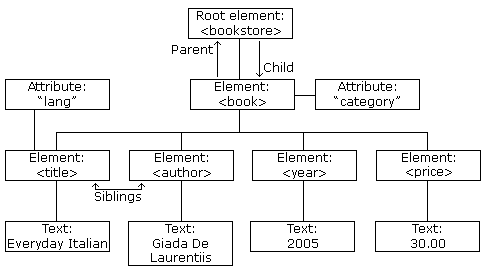
\includegraphics[width=\textwidth]{figures/nodetree}
\caption{Raamatupoe hierarhiline struktuur \citep{XML}}
\end{figure}

Joonise 1 kujutamine XML-kujul:


\begin{lstlisting}
<?xml version="1.0" encoding="UTF-8"?>
<bookstore>
  <book category="cooking">
    <title lang="en">Everyday Italian</title>
    <author>Giada De Laurentiis</author>
    <year>2005</year>
    <price>30.00</price>
  </book>
  <book category="children">
    <title lang="en">Harry Potter</title>
    <author>J K. Rowling</author>
    <year>2005</year>
    <price>29.99</price>
  </book>
  <book category="web">
    <title lang="en">Learning XML</title>
    <author>Erik T. Ray</author>
    <year>2003</year>
    <price>39.95</price>
  </book>
</bookstore>
\end{lstlisting}
\citep{XML}

XML-i võib vaadata kui reeglite kogumikku, milles talletatakse informatsiooni semantiliste märgendite abil. Märgendid (\emph{tags}) on \emph{<>} märkide vahel olevad muutujad ja igal märgendil peab olema lõpumärgend (nt \emph{<bookstore>} ja \emph{</bookstore>}). XML dokument koosneb kolmest osast: proloog, dokumendi element ja epiloog. Faili alustatakse proloogiga, mis defineerib XML-i versiooni ja kasutatava kodeeringu. Dokumendi element on juurelement, mida saab olla vaid üks. Joonise 1 juurelement on \emph{<bookstore>}, mille alluvaks on elemendid \emph{<book>}. Märgenditel võib olla atribuut kui ka sisu, kuid need pole ilmtingimata kohustuslikud. Selles XML-koodijupis on raamatutel defineeritud ka atribuut \emph{category}, mille väärtus oleneb raamatu valdkonnast. Elemendi \emph{<book>} alluvateks on \emph{<title>}, \emph{<author>}, \emph{<year>} ja \emph{<price>}, mis on omakorda teineteise kolleegid. Kõigil neil elementidel on sisu ja elemendil \emph{<title>} on ka atribuut \emph{lang}, mille väärtuseks on keel. Viimane rida (\emph{</bookstore>}) ütleb, et see on juurelemendi lõpp ja ühtlasi ka dokumendi keha lõpp. See tähendab, et rohkem raamatuid selles raamatupoes ei eksisteeri. \citep{XML}

Märgendite abil pannakse paika andmete loogiline struktuur. XML-il pole eeldefineeritud märgendeid. Seega igal inimesel on võimalik defineerida oma vajadustele vastav struktuur ehk süntaks, mis paneb paika elemendi nimetused ja järjestuse. Oluline on, et kasutaja poolt defineeritud süntaks vastaks XML-i rangetele reeglitele:

\begin{enumerate}
    \item eksisteerib juurelement;
    \item elementidel peab olema lõpumärgend;
    \item elementide pesitsemine ehk üksteise sees paiknemine (\emph{nesting}) on rangelt määratletud;
    \item atribuutide väärtused peavad olema jutumärkides.
    \citep{XML}
\end{enumerate}

Kui kasutaja loob enda märgenduse, siis XML-protsessoril pole võimalik selle valiidsuses veenduda, sest pole midagi millegagi võrrelda. Selleks tuleb kasutajal XML-dokumendis defineerida kasutatav süntaks. XML-dokumentide valideerimiseks on kaks viisi: dokumenditüübi definitsioon (\emph{document type definition} -- DTD) ja XML-skeema (\emph{XML schema}). Nende asukoht on vahetult peale XML-versiooni deklaratsiooni ja kindlasti enne dokumendi keha. Juhul kui XML-doku\-ment on DTD või XML skeemaga vastavuses, siis on ka XML-dokument kehtiv. \citep{XML}

Sellisel markeerimiskeelel on küll palju eeliseid, kuid puudusteks peetakse seda, et see on verboosne (nt kohustuslik lõpumärgend), nõuab kõrget valideerimisstandardit ja elemendid peavad rangelt üksteise sees paiknema. Näiteks suulises kõnes on palju pealerääkimisi, kuid vastavalt XML-i rangetele reeglitele pole elementide ristumine võimalik. Oma XML-i süntaksi kirjutamine pole lihtne (kõigi eelnevalt nimetatud puuduste tõttu), seega eelistavad inimesed kasutada juba teada tuntud kodeerimisskeemasid (nt CHILDES, Brown jne). \citep{LEECH}

\subsubsection{Morfoloogiline analüüs}

Morfoloogilise analüüsi käigus lisatakse iga sõna jaoks infot selle lemma ehk algvormi, sõnaliigi ja morfoloogiliste kategooriate kohta: käändsõnal arv ja kääne, tegusõnal pööre, tegumood, aeg, kõneviis, kõneliik. Teksti morfoloogiliseks analüüsimiseks kasutatakse morfoloogilist analüsaatorit. Analüsaator on programm, mis saab sisendiks teksti ja mille väljundiks on morfoloogiliselt analüüsitud sõnad. \citep[89]{KV}

Morfoloogiline analüüs koosneb kahest etapist -- üksiksõnade analüüsimine ja ühestamine. Analüsaator annab igale sõnale selle interpretatsioonid ehk analüüsivariandid. Seejärel toimub morfoloogiline ühestamine. Morfoloogiliseks ühestamiseks nimetatakse protsessi, kus kõikvõimalikest interpretatsioonidest tuleb välja valida antud konteksti sobiv analüüs.\citep[90]{KV}

Selles magistritöös kasutatakse lapsekeele korpuse morfoloogiliseks analüüsimiseks sõnastikupõhist morfoloogilist analüsaatorit. Sõnastikupõhisel morfoloogilisel analüüsimisel töödeldakse sõnavorme ja võrreldakse antud keele leksikoniga, juhul kui sõna leksikonis pole, siis kasutatakse mitmesuguseid heuristilisi reegleid. Sõnastikus eristatakse sõnaliike järgnevalt:


\begin{itemize}
    \item A = adjektiiv - algvõrre e positiiv;
    \item C = adjektiiv - keskvõrre e komparatiiv;
    \item D = määrsõna (e adverb);
    \item G = genitiivatribuut (käändumatu omadussõna);
    \item H = pärisnimi;
    \item I = hüüdsõna (e interjektsioon);
    \item J = sidesõna (e konjunktsioon);
    \item K = kaassõna (pre/postpositsioon);
    \item N = põhiarvsõna (e kardinaalnumeraal);
    \item O = järgarvsõna (e ordinaalnumeraal);
    \item P = asesõna (e pronoomen);
    \item S = nimisõna (e substantiiv);
    \item U = adjektiiv - ülivõrre e superlatiiv;
    \item V = tegusõna (e verb);
    \item X = verbi juurde kuuluv sõna, millel eraldi sõnaliigi tähistus puudub;
    \item Y = lühend;
    \item Z = lausemärk. \citep{VABAMORF}
\end{itemize}


98\% eesti keele sisendteksti sõnadest on analüüsitavad nii, et kasutatakse sõnastikku, morfeemide loendeid ja nende kombineerimise eeskirju. Sõnadel lõigatakse maha lõpud ja liited ning võrreldakse sõnastikus olevate lekseemidega. Kuni 3\% teksti sõnadest pole sõnastikupõhiselt võimalik analüüsida, sest sõnastikus puudub selle kohta kirje. Oletamisega oletatakse sõna algvorm ja selle vorm puhtalt sõnavormi alusel. Paraku analüsaator ei paku alati õigeid analüüsivariante (vale analüüse kuni 0,1\%) ja selle peamised vead seisnevad selles, et sisendtekst pole analüsaatori jaoks mõeldud (analüsaator on mõeldud kirjakeele analüüsimiseks) ja et pärisnimed sarnanevad vormilt üldnimisõnadega. \citep[91--93]{KV}


\newpage
\section{CHILDES ja eesti keele alamkorpused}

Selles peatükis tutvustatakse CHILDES-i korpust ja eesti lapsekeele korpuste struktuuri, mida siinkirjutaja kasutab magistritöö andmestikuna. Lisaks antakse lühiülevaade alamkorpuste standardiseerimise probleemidest.

\subsection{CHILDES}
CHILDES (\emph{Child Language Data Exchange System}) on \emph{Talkbank}i alamkorpus, mis loodi 1984. aastal Brian MacWhinney (Carnagie Melloni ülikool) ja Catherine Snow (Harvardi ülikool) poolt selleks, et koondada kokku erinevate keeleuurijate kogutud keelematerjali eesmärgiga, et need oleksid kõigile vabalt kättesaadavad ja võimaldaksid eri keelte uurijatel oma andmeid ja uurimistulemusi teiste keeltega võrrelda. CHILDES-ist on saanud mahukas, rahvusvaheline ja usaldusväärne andmebaas, mis sisaldab nii audio- ja videolindistusi kui ka standardsel viisil transkribeeritud tekste. \citep[1]{Gillis}

CHILDES-i süsteemi juures peab silmas pidama seda, et see funktsioneerib \emph{repositooriumina}. Repositooriumist võib mõelda kui laost või arhiivist, kuhu üles laetud materjali talletatakse digitaalselt. Repositooriumi jaoks on oluline, et korpused oleksid avalikult kättesaadavad ja standardsel viisil transkribeeritud ja et andmekogu oleks kooskõlas rahvusvaheliste standarditega. Seetõttu pakub CHILDES erinevaid tarkvaralisi töövahendeid, mida arendatakse ja kaasajastatakse kõigil platvormidel (\emph{Windows}, \emph{MacOS}, \emph{Unix}). \citep[1]{Gillis}

CHILDES-i andmebaas jaguneb nelja suurde kategooriasse:
\begin{enumerate}
    \item esimese keele omandamine;
    \item teise keele keele omandamine;
    \item kakskeelsus ja 
    \item kliinilised probleemid. \citep[1]{Gillis}
\end{enumerate}

Andmebaasi tekstide/lindistuste transkribeerimiseks ja kodeerimiseks kasutatakse CHAT käsiraamatut (\emph{Codes of the Human Analysis of Transcripts}, vt \citep{CHAT}). CHAT käsiraamat on mõeldud selleks, et kõik lindistused/tekstid oleksid standardsel viisil transkribeeritud ja kodeeritud. Käsiraamatus on väga suur valik kodeeringuid, kuid transkribeerija ei ole kohustatud neid kõiki kasutama. Oluline oleks, et transkribeerimist ja kodeerimist tehakse vähemalt baastasemel. Lisaks CHAT käsiraamatule on keeleuurijatel võimalus kasutada ka analüüsimistarkvara ja redaktorit CLAN (\emph{Computerized Language Analysis}), mis abistab keeleuurijat korpuse transkribeerimisel, kodeerimisel ja analüüsimisel. CLAN võimaldab analüüsida kollokatsioone, sõna- ja foneemisagedusi, arvutada vormide ja lausungite keskmisi pikkusi. CLAN tarkvaraga loodud failiformaati nimetatakse CHAT-failiks ja see salvestatakse laiendiga .\emph{cha} (xxx.cha) \citep[1--2, 6]{Gillis} Talkbankis on kasutusel ka Chatter tarkvara, mis teostab CHAT-failide ranget valideerimist ja ka konverteerimist valiidseteks XML-failideks \citep{CHATTER}.

Hetkel on andmebaasis esindatud 39 keelt ja 2013. aasta maikuu seisuga koosnes andmebaas 13 miljonist lausungist ja rohkem kui 50 miljonist sõnavormist. Kõige suurema mahuga on esimesse kategooriasse kuuluvad ehk esimese keele korpused (11 miljonit lausungit ja 43 miljonit sõnavormi). Kõige suurema esindatavusega on inglise, saksa ja prantsuse keel.\citep[2--5]{Gillis}

Transkriptsioonid algavad päisega (ingl k. \emph{header}), kus antakse informatsiooni lindistuse aja, koha, osalejate, kestuse, laste vanuse jms kohta. Põhiridadele paigutatakse kõnelejat tähistav kolmetäheline kood, millele järgneb  kõneleja tegelik kõne. Tegelikule kõnele lisatakse juurde, kas transkribeerija- või uurijapoolsed kommentaarid või kodeeringud (neid nimetatakse \emph{sõltridadeks}). Sõltridade arv oleneb keeleuurija eesmärkidest. Nagu suulise kõne puhulgi, pole ainuüksi verbaalse info järgi aru saada, millest hetkel jutt käib, seega tuleks transkribeerimisel kasutada vähemalt üht sõltrida, nt kommentaaririda. (\citealp[68]{Argus2007}; \citealp{CHAT}) Vt näide (1) ja (2).
\hfill

(1):
\begin{description}
    \item*MOT: arvuta need kõigepealt ära.
    \item*CHI: jah mm kaheksa miinus seitse on üks.
    \item*CHI: niimoodi kümme miinus üks on üheksa.
    \item\%com CHI kirjutab ja ise räägib samal ajal kaasa.
    \item(Kõrgesaar, gregory03.cha)
\end{description}
\hfill

(2)
\begin{description}
    \item*FAT:   köögis saab teritada , köögis on nuga .
    \item*MOT:   +< aga siin oli ka teritaja .
    \item*FAT:   jaa aga ma ei tea , kus see on .
    \item*CHI:   +< seda kätte .
    \item*FAT:   mida sa tahad kätte , issi ei tea , kus see teritaja on .
    \item*MOT:   see teritas väga ilusasti muidu .
    \item*CHI:   telita [*] .
    \item\%err:   terita=teritaja \$MOR
    \item\%par:   CHI aevastab
    \item(Vija, 20008.cha)
\end{description}


\subsection{Alamkorpuste standardiseerimise probleemid}

Reili Argus kirjeldab oma artiklis \citep{Argus2007} mõningaid transkribeerimise ja CHILDES-i tarkvara kasutamisega seonduvaid probleeme. Esiteks, analüüsitarkvara CLAN on mõeldud inglise keelele, seega tuleb eesti keele analüüsimisel arvestada sellega, et eesti keel on võrreldes inglise keelega sünteetilisema süsteemiga keel. Seega, kui keeleuurija tahab CLAN-i kasutades teha mingisuguseid sagedusloendeid, siis ei saada adekvaatseid tulemusi. Näiteks lekseemi \emph{kala} kolm sõnavormi \emph{kala}, \emph{kalaga}, \emph{kalale} loetakse programmi poolt eri lekseemideks. Selline asjaolu põhjustab ka statistiliselt väärate arvude tekkimist. Homonüümide eristamist tuleb teha näiteks käsitsi.\citep[70]{Argus2007}

Argus väidab, et kuna lindistuste transkribeerimisel kasutatakse kuuldeortograafiat, siis need transkriptsioonid ei anna tõetruud pilti sellest, milline on lapse tegelik keelekasutus. Kui juba suulise kõne automaatne analüüsimine on keeruline, siis on lapse suulise keele analüüsimine veel keerukam. Lindistuste puhul on tegemist spontaanse suulise kõnega, mis sisaldab elemente, mida pole tarvis analüüsida, nt häälitsused. Seega selleks, et korpuseid oleks võimalik analüüsida nii, et need annaksid keelekasutuse kohta autentse pildi, ja et oleks võimalik neid standardsele kujule viia, tuleb alustada juba korpuse tekstide transkribeerimise tasandist. \citep[71]{Argus2007}

Teiseks, probleeme tekitab see, et lapse puhul on tegemist ju areneva keelekasutusega, milles esineb palju erilisi tunnuseid, nt sõnakordus. Näiteks, kui sellist lausungit transkribeeritakse nii \emph{*CHI: onu, onu, onu}, siis tähendab see seda, et lapse lausung koosneb kolmest sõnavormist, aga kui näiteks transkribeerida seda lausungit viisil \emph{*CHI: onu [/] onu [/] onu [/]}, siis koosneb see lausung ühest sõnavormist, kuna CLAN tarkvara kohtleb seda kui korduvat üksust. Lisaks sõnakordusele on probleemiks ka onomatopoeetilised sõnad, mida esineb lapsekeeles väga palju ja seetõttu tuleb transkribeerimisel läbi mõelda, kuidas selliseid juhtumeid lahendada. CHAT käsiraamat soovitab onomatopoeetiliste sõnade lõppu lisada sümbol \emph{@} \citep[72--73]{Argus2007}, aga reaalsuses kasutatakse seda ikka väga vähe ja see omakorda põhjustab seda, et transkriptsioonid ei järgi ühtset märgendamisstiili.

Võrreldes täiskasvanutega esineb lapsekeeles rohkem vigaseid vorme. Transkribeerimisel (nt vigade korral) on oluline, et transkribeerija peab nägema ja teadma seda, mida tegelikult öelda taheti, ja vastavad kodeeringud ka transkriptsiooni lisama nii, et need oleksid juba esimesel tasandil liigitatud. \citep[74]{Argus2007} Kahjuks praegused alamkorpused pole veakodeerimise osas järjepidevad, kord on viga kodeeritud ühtmoodi, kord teistmoodi ja vahel üldse mitte. Näites (2) on viga põhireal kodeeritud kooloniga (\emph{:}), mille järele lisatakse korrektne sõnavorm. Näites (3) on veakodeerimine hoopis teine: põhireal järgneb vigasele sõnale [*] ja sõltreale on lisatud vearida (\emph{\%err}), kus  toimub vea lahtikodeerimine ja sümboli \emph{=} järele lisatakse korrektne vorm. Näites (4) on viga üldse kodeerimata jäetud.
\hfill

(2)
\begin{description}
    \item*FAT: kriit pane tahvli peale .
    \item*CHI: kit [: kriit] .
    \item*CHI: kit [: kriit] (.) vahvlile [= tahvlile] pääle [: peale] .
    \item(Vija; 20007.cha)
\end{description}
\hfill

(3)
\begin{description}
    \item*CHI: issi , loe seda .
    \item*CHI: issi , nüüd see [*] ei pane kinni !
    \item\%err: see=seda \$MOR
    \item(Vija; 20007.cha)
\end{description}
\hfill

(4)
\begin{description}
    \item*FAT: viskad minema või?
    \item*FAT: kus sa viskad selle?
    \item*CHI: kinn.
    \item*FAT: sinna viskad jah.
    \item(Kõrgesaar; arabella01f.cha)
\end{description}
\hfill


Morfoloogiliselt märgendatud korpuse loomine on väga vajalik, sest CHILDES-i analüüsitarkvara ei võimalda eesti keele morfoloogilist analüüsimist ja selle käsitsi tegemine oleks väga ajamahukas töö. Seega, praegusel hetkel on lapsekeele uurijatel automaatse statistika tegemine raskendatud ja paraku tehakse distributsioonianalüüse käsitsi \citep[78]{Argus2007}.

\subsection{Eesti keele alamkorpuste struktuur}

Selles töös kasutatakse kolm keskset mõistet -- \emph{sõna}, \emph{sõnavorm} ja \emph{sõnavara}. Sõna all mõeldakse tekstisõna ehk tühikute vahele jäävat tähtede järjendit, nt lauses \emph{võtan teise pliiatsi} koosneb kolmest sõnast. Sõnavorm on unikaalne tekstisõna, nt lauses \emph{pliiats ja pliiatsiga} on kaks sõnavormi (need on ühe ja sama lekseemi \emph{pliiats} erinevad grammatilised vormid, siis selles töös käsitletakse neid kui kaht eri sõna); lauses \emph{punane pliiats ja roheline pliiats} on sõnavorme kokku neli. Sõnavara puhul on oluline rõhutada, et selles töös räägitakse sõnavarast kui leksikonist, mida hinnatakse sõnavormide alusel. Oletame, et lapse repertuaaris on vaid üks lause \emph{võtan punase pliiatsi ja rohelise pliiatsi}, siis selle lapse sõnavara suurus on 5 sõna.

CHILDES-i andmebaasis on eesti laste suulise kõne lindistused olnud alates 1998. aastast. 2016. aasta märtsikuu seisuga koosneb eesti lapsekeele korpus seitsmest alamkorpusest, mis on oma nimed saanud korpuse koostajate järgi: Argus, Beek, Kapanen, Kohler, Kõrgesaar, Vija ja Zupping \citep{CHILDES}. Arguse, Beeki, Kapaneni, Vija ja Zuppingu korpustes on andmete kogumiseks kasutatud longituuduurimusele omast viisi, kus teatud perioodi jooksul salvestatakse lapse ja hoidja vestlusi intensiivselt ja mille tulemusena tekib tihe andmestik. Kohleri ja Kõrgesaare korpustes pärinevad andmed salvestustest mitme eri vanuses lapsega. Lisades 1--6 on iga alamkorpuse kohta koondlikult välja toodud lapse nimi, vanus, sugu, sessioonide arv, lapse ja hoidja sõnade koguarv igas vanuses.

Kõikides alamkorpustes on alamkorpuse sõnade koguarvu poolest ülekaalus hoidja sõnad, mis on küllatki ootuspärane tulemus (vt joonis 2).

\begin{figure}[H]
    \centering
    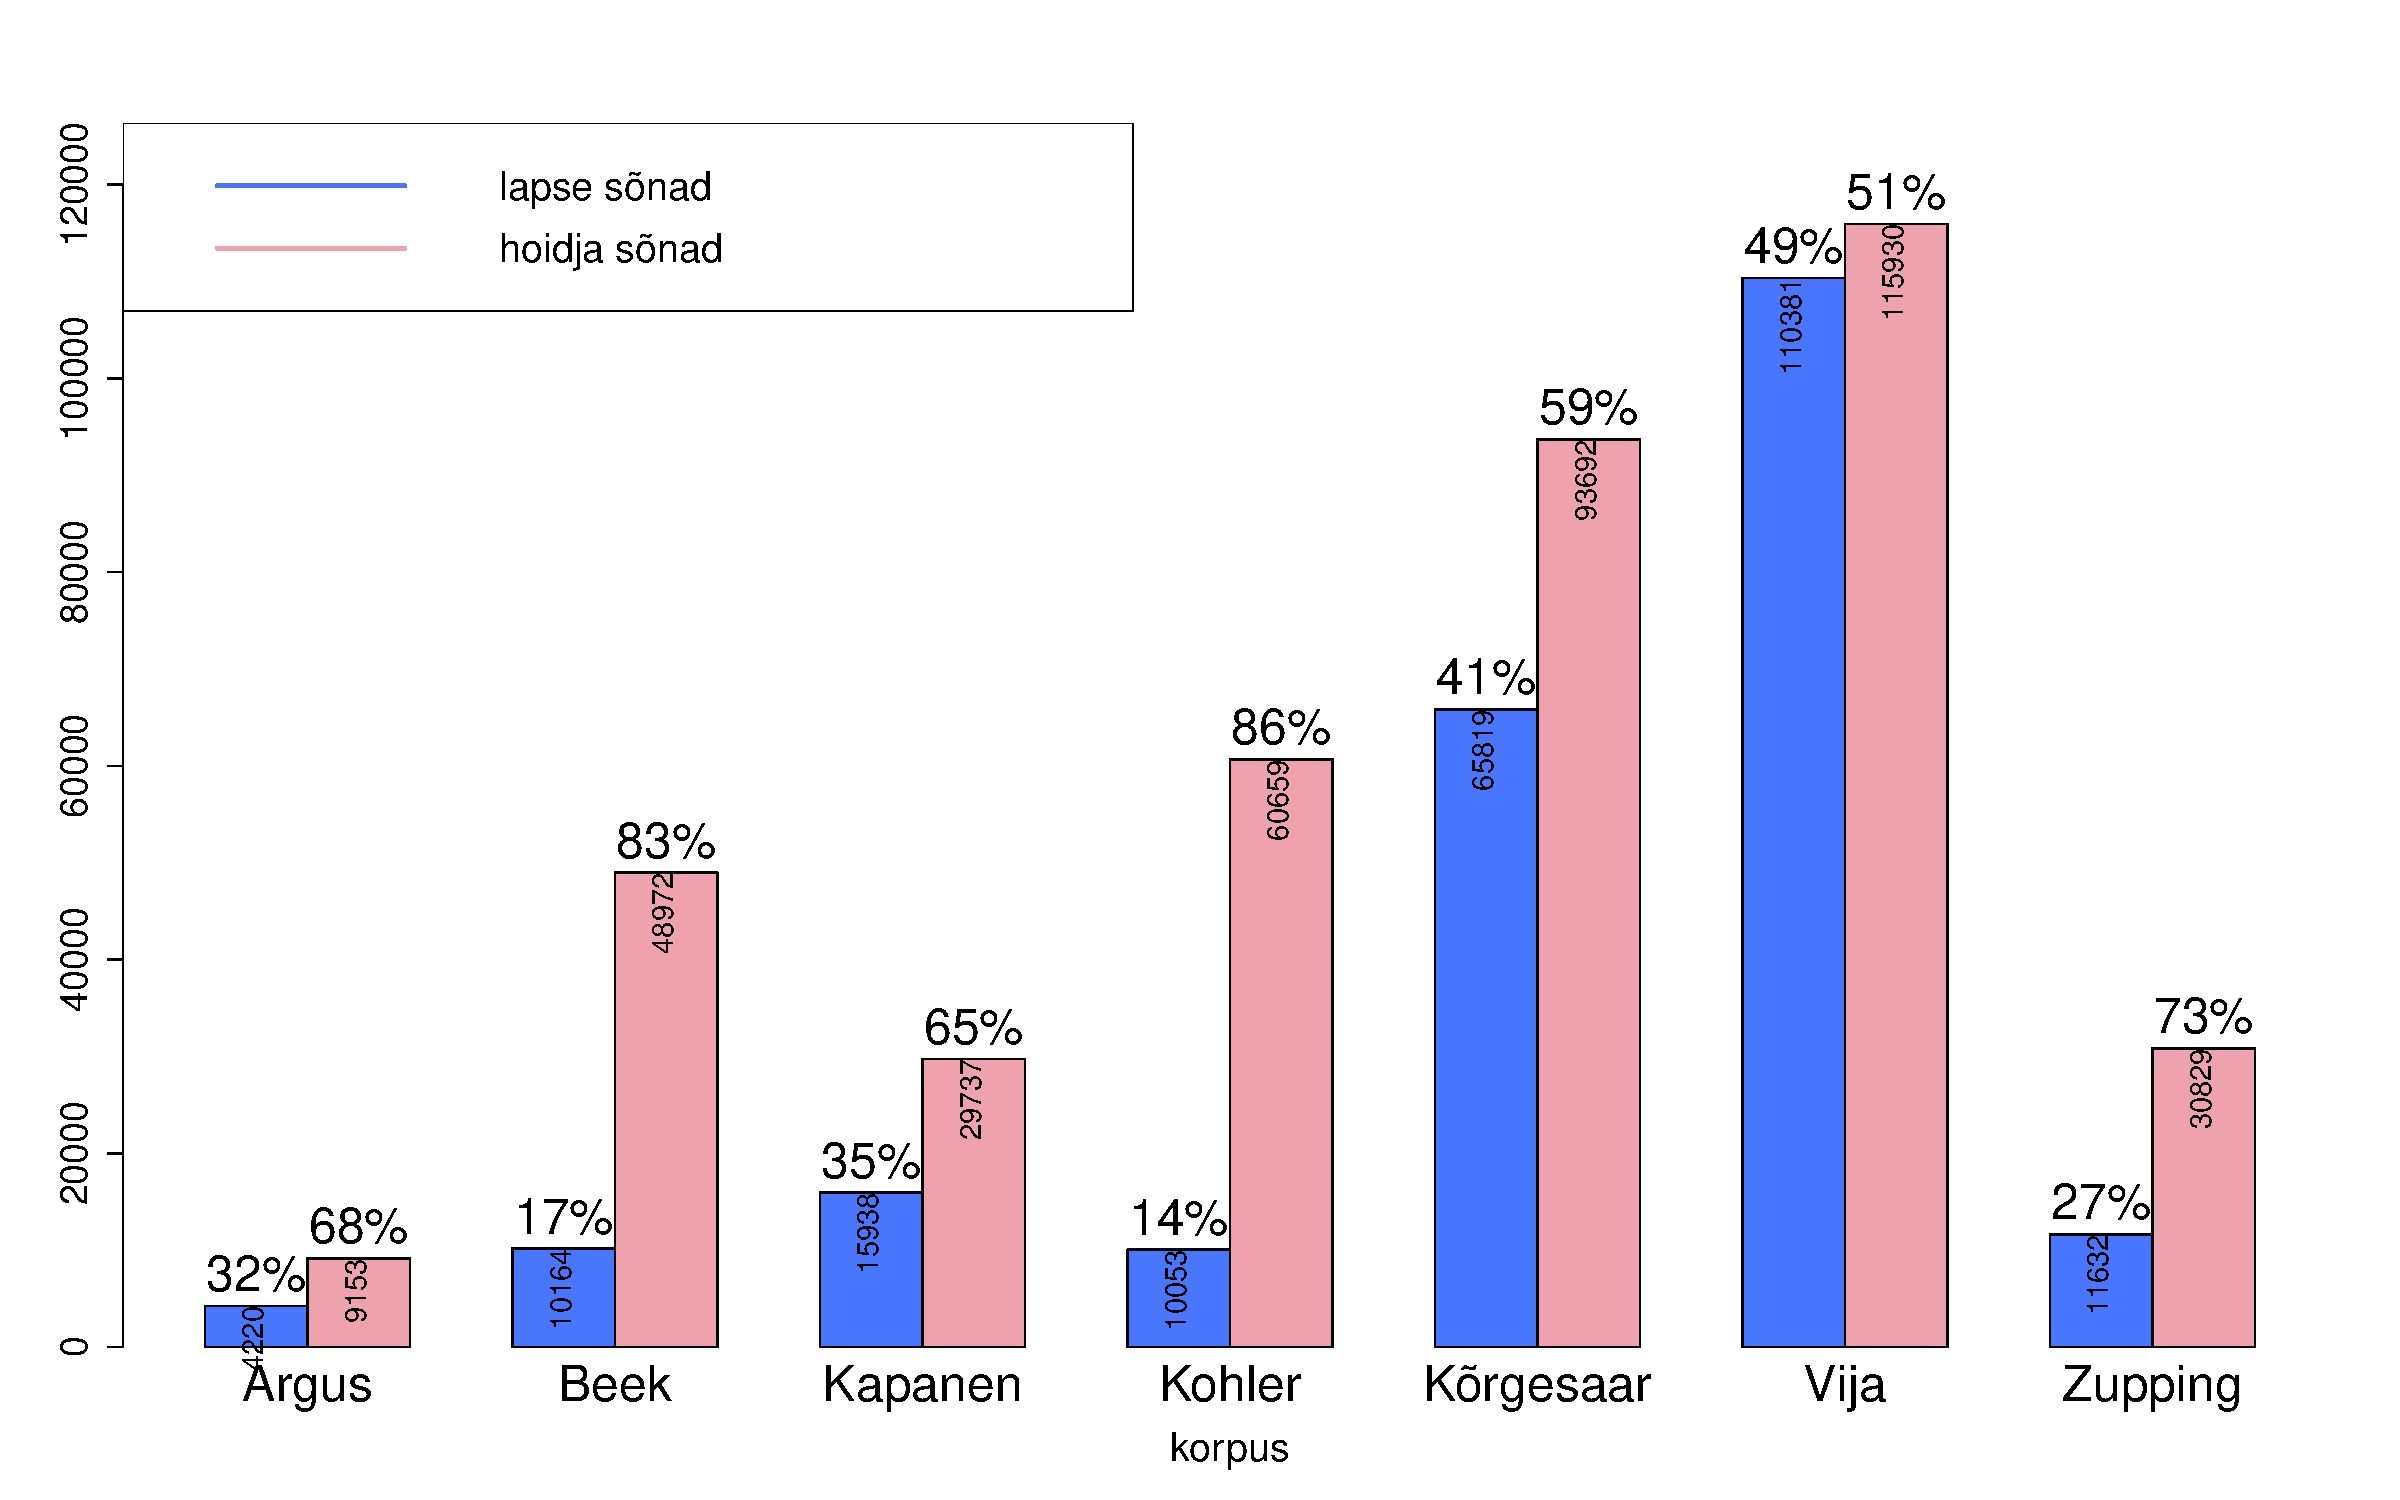
\includegraphics[width=\textwidth]{koik_korpus_sonad}
    \caption{hoidja ja lapse sõnade jaotumine alamkorpustes}
\end{figure}

Kõige mahukamad on Vija, Kõrgesaare ja Kohleri alamkorpused. Neist mahukaim on Vija korpus (vt joonis 2 ja lisa 1), sisaldades 226311 sõna, millest 49\% (110381 sõna) olid lapse sõnad ja hoidja sõnad 51\% (115930 sõna). Lindistusi tehti Andreasega vahemikus 1;7--3;1 eluaastat. Kõrgesaare korpus (vt ka lisa 5) koosneb 159511 sõnast, neist 41\% (65819) on lapse sõnad ja 59\% (93692) hoidja sõnad. Materjal pärineb lindistustest 12 erineva lapsega vahemikus 1;3--14;1 eluaastat. Siia pole sisse arvestatud transkriptsioone vestlustest, mille osalejateks olid vaid täiskasvanud. Kohleri korpus (vt ka lisa 7) sisaldab 70712 sõna, kus lapse sõnad moodustavad 14\% (10053 sõna) ja hoidja sõnad 86\% (60659 sõna). Lindistusi tehti 8 erineva lapsega vahemikus 0;11--2;3 eluaastat.

Beeki korpus (vt ka lisa 3) sisaldab 59136 sõna, millest lapse sõnad moodustavad 17\% (10164 sõna) ja hoidja sõnad 83\% (48972). Lindistusi tehti Liisbetiga vahemikus 0;9--2;5 eluaastat. Kapaneni korpus (vt ka lisa 4) koosneb 45675 sõnast, neist 35\% (15938 sõna) on lapse sõnad ja 65\% (29737) hoidja sõnad. Kapaneni materjal pärineb lindistustest Martinaga vahemikus 1;3--2;7 eluaastat. Zuppingu korpus (vt ka lisa 6) sisaldab 42461 sõna, neist 27\% (11632) on lapse sõnad ja 73\% (30829) hoidja sõnad. Kõik lindistused on tehtud Lindaga vahemikus 1;3--4;2 eluaastat. Mahult kõige väiksem on Arguse korpus (vt ka lisa 2). Korpus sisaldab 13373 sõna, millest 32\% (4220) on lapse ja 68\% (9153) hoidja sõnad. Lindistusi tehti Hendrikuga vahemikus 1;8--2;5 eluaastat.

Tabel 1 näitab, kuidas jaotuvad kogu korpuse lapse ja hoidja sõnad alamkorpuste kaupa.

\begin{table}[H]
\centering
\caption{lapse ja hoidja sõnade \% kogu korpuses}
\begin{tabular}{|l|c|c|c|c|}
\hline
korpus                 & \multicolumn{1}{l|}{lapse sõnad}                                       & \multicolumn{1}{l|}{\% kogu korpuses} & \multicolumn{1}{l|}{hoidja sõnad}                                      & \multicolumn{1}{l|}{\% kogu korpuses} \\ \hline\hline
Vija                   & 110381                                                                 & 48\%                                   & 115930                                                                 & 30\%                                   \\ \hline
Kõrgesaar              & 65819                                                                  & 29\%                                   & 93692                                                                  & 24\%                                   \\ \hline
Argus                  & 4220                                                                   & 2\%                                    & 9153                                                                   & 2\%                                    \\ \hline
Beek                   & 10164                                                                  & 4\%                                    & 48972                                                                  & 13\%                                   \\ \hline
Kapanen                & 15938                                                                  & 7\%                                    & 29737                                                                  & 8\%                                    \\ \hline
Zupping                & 11632                                                                  & 5\%                                    & 30829                                                                  & 8\%                                    \\ \hline
Kohler                 & 10053                                                                  & 4\%                                    & 60659                                                                  & 16\%                                   \\ \hline\hline
\multirow{2}{*}{KOKKU} & \multirow{2}{*}{\begin{tabular}[c]{@{}c@{}}228207\\ 37\%\end{tabular}} & \multirow{2}{*}{100\%}                 & \multirow{2}{*}{\begin{tabular}[c]{@{}c@{}}388972\\ 63\%\end{tabular}} & \multirow{2}{*}{100\%}                 \\
                       &                                                                        &                                        &                                                                        &                                        \\ \hline
\end{tabular}
\end{table}

Kogu korpuses moodustavad lapse sõnad 37\% (228207 sõna) ja hoidja sõnad 63\% (388972 sõna). Korpuse suuruseks on 617179 sõna. Kogu korpuses on Vija alamkorpus nii lapse kui hoidja sõnade poolest kõige suurema osakaaluga: lapse sõnad moodustavad 48\% kõigi laste sõnade arvust, hoidja sõnad 30\% kõigi hoidja sõnade arvust (vt tabel 1). Kõrgesaare alamkorpus moodustab kõigi laste sõnade arvust 29\%, hoidja sõnad 24\% kõigi hoidja sõnade arvust. Kohleri alamkorpuse lapse sõnad moodustavad 4\% kõigi laste sõnade arvust, hoidja sõnad 16\% kõigi hoidja sõnade arvust. Beeki alamkorpuse lapse sõnad moodustavad 4\% kõigi laste sõnade arvust, hoidja sõnad 13\% kõigi hoidja sõnade arvust.

Kapaneni alamkorpuse lapse sõnad moodustavad 7\% kõigi laste sõnade arvust, hoidja sõnad 8\% kõigi hoidja sõnade arvust. Zuppingu alamkorpuse lapse sõnad moodustavad 5\% kõigi laste sõnade arvust, hoidja sõnad 8\% kõigi hoidja sõnade arvust. Arguse alamkorpuse lapse sõnad moodustavad 2\% kõigi laste sõnade arvust, hoidja sõnad samuti 2\% kõigi hoidja sõnade arvust.

Korpuse üks koostamise põhimõte on, et korpus peab olema representatiivne ehk uuritava nähtuse suhtes esinduslik. Kui me uurime nii lapse kui hoidja keelekasutust, siis tuleb teada, kelle keelekasutust korpus esindab. Joonis 3 illustreerib seda, kuidas jaotuvad lapse ja hoidja sõnad kogu korpuses. Me näeme, et suurem osa transkriptsioonidest on tehtud vanuses 1 kuni 3. See tähendab, et korpuses on suur hulk sõnu, mis esindavad vaid teatud vanusegruppe ja see omakorda peegeldab paljude teiste vanusegruppide esinduslikkust.

\begin{figure}[H]
    \centering
    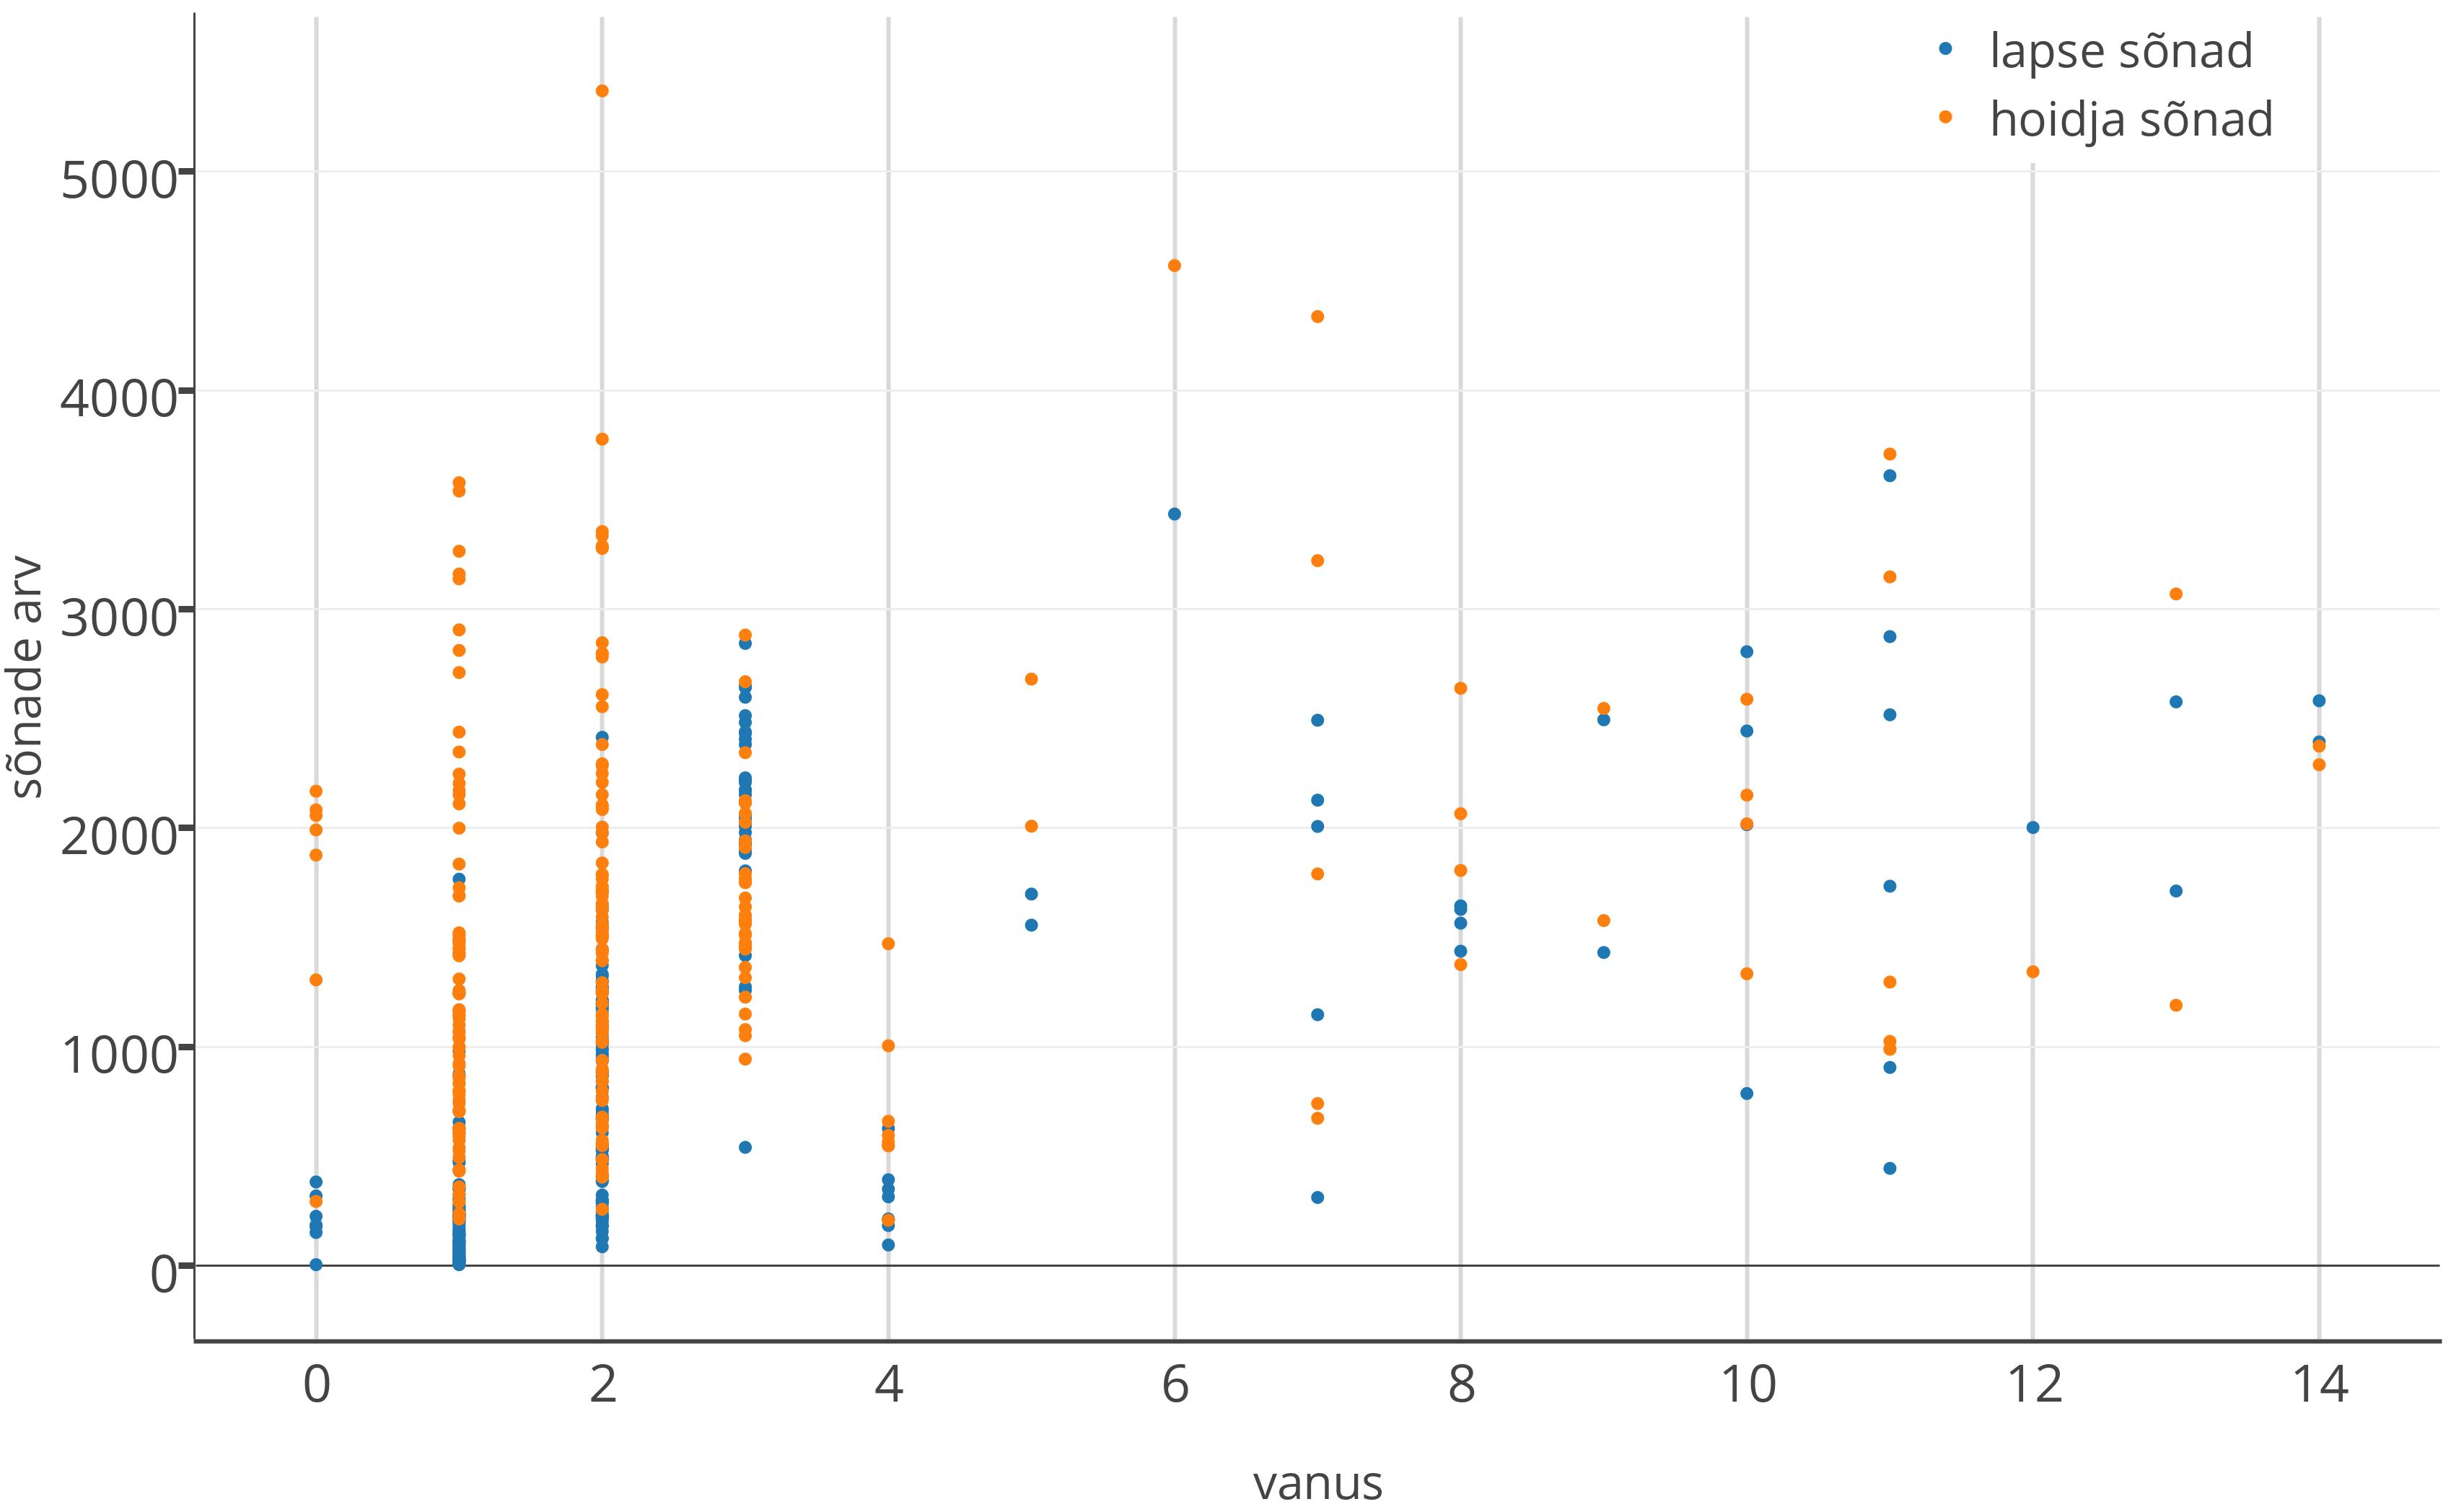
\includegraphics[width=\textwidth, height=9cm]{lindistused_vanus_sonad_crop}
    \caption{hoidja ja lapse sõnade jaotumine kogu korpuses vanuse järgi}
\end{figure}

Kui vaadata detailsemalt lapse ja hoidja sõnade jaotumist vanusegrupiti, siis kogu korpus esindab 2- ja 3-aastaste laste keelekasutust (vt joonis 4 (a)). Ülejäänud vanusegrupid (ehk 86\% kõikidest vanusegruppidest) esindavad korpuses lapse sõnu vaid 35,8\%. Hoidja sõnadest (vt joonis 4 (b)) on kõige suurema osakaaluga 2-aastaste (37,4\%), 1-aastaste (27,7\%) ja 3-aastaste (14,6\%) vanusegrupp. Ülejäänud vanusegrupid (ehk 80\%) esindavad hoidjate sõnadest vaid 20,3\%. Selline tulemus on loogiliselt põhjendatav: mida rohkem sessioone, seda rohkem sõnu ja seda suurem korpus. Kõigis alamkorpustes tehti kõige enam lindistusi just 1-, 2- ja 3-aastaste lastega.

Korpus esindab enam-jaolt Andrease (Vija korpus) ja tema hoidja keelekasutust, sest Andrease sõnad moodustavad kõikide laste sõnadest lausa 48,4\% ja Andrease hoidja sõnad kõikidest hoidja sõnadest 29,8\% (vt joonis 5 (a) ja (b)). See tähendab, et ülejäänud lapsed (ehk 96\%) esindavad kogu korpuses lapse keelekasutust vaid natuke üle 50\%. Ja nendest ülejäänud lastest 56\% (ehk 14 last 25 lapsest) esindavad korpuses vähem kui 1\%. Hoidjate keelekasutus varieerub natuke rohkem: kogu korpuses esindab ülejäänud hoidjate keelekasutus 70,2\%, kuid hoidjatest 32\% (ehk 8 hoidjat 25 hoidjast) esindab kogu korpuses vähem kui 1\% hoidja sõnu. Ka siin mängivad olulist rolli lapsega tehtud sessioonide arv ja korpuse suurus. Näiteks Vija korpuse puhul on tegemist tiheda andmestikuga, kus Andreasega tehti kokku 74 sessiooni, kuid Kõrgesaare korpuses tehti Sirlini, Arturi ja Arabellaga vaid 1 sessioon, mistõttu on kogu korpuses nende laste keelekasutuse osakaal miniatuurne.

\begin{figure}[H]
    \centering
    \subfloat[lapse sõnad]{{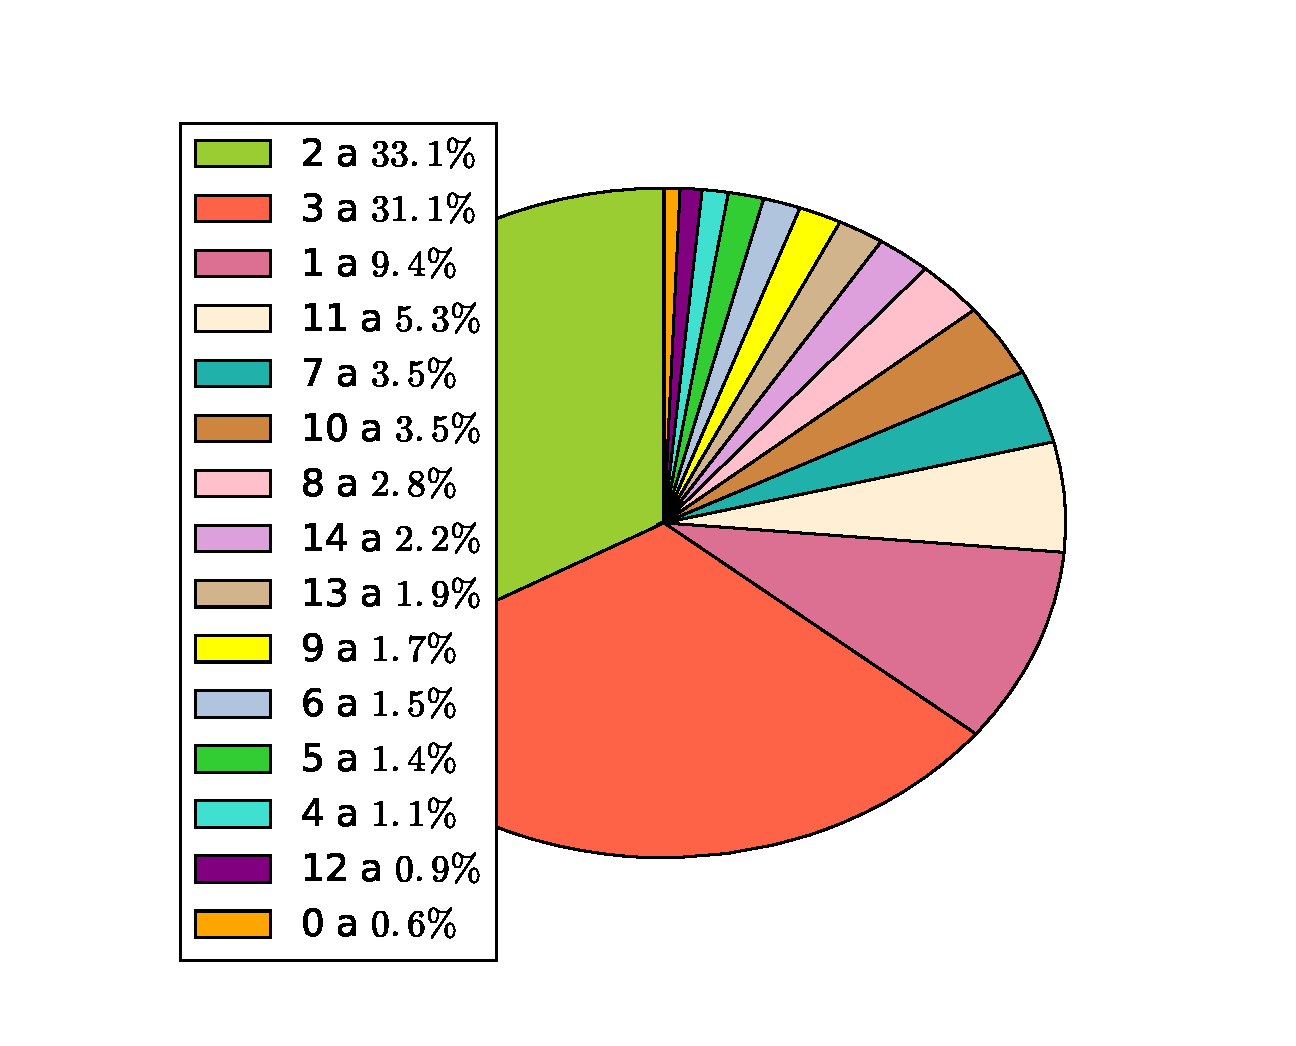
\includegraphics[width=10cm]{vanus_laps_sonad} }}
    \qquad
    \subfloat[hoidja sõnad]{{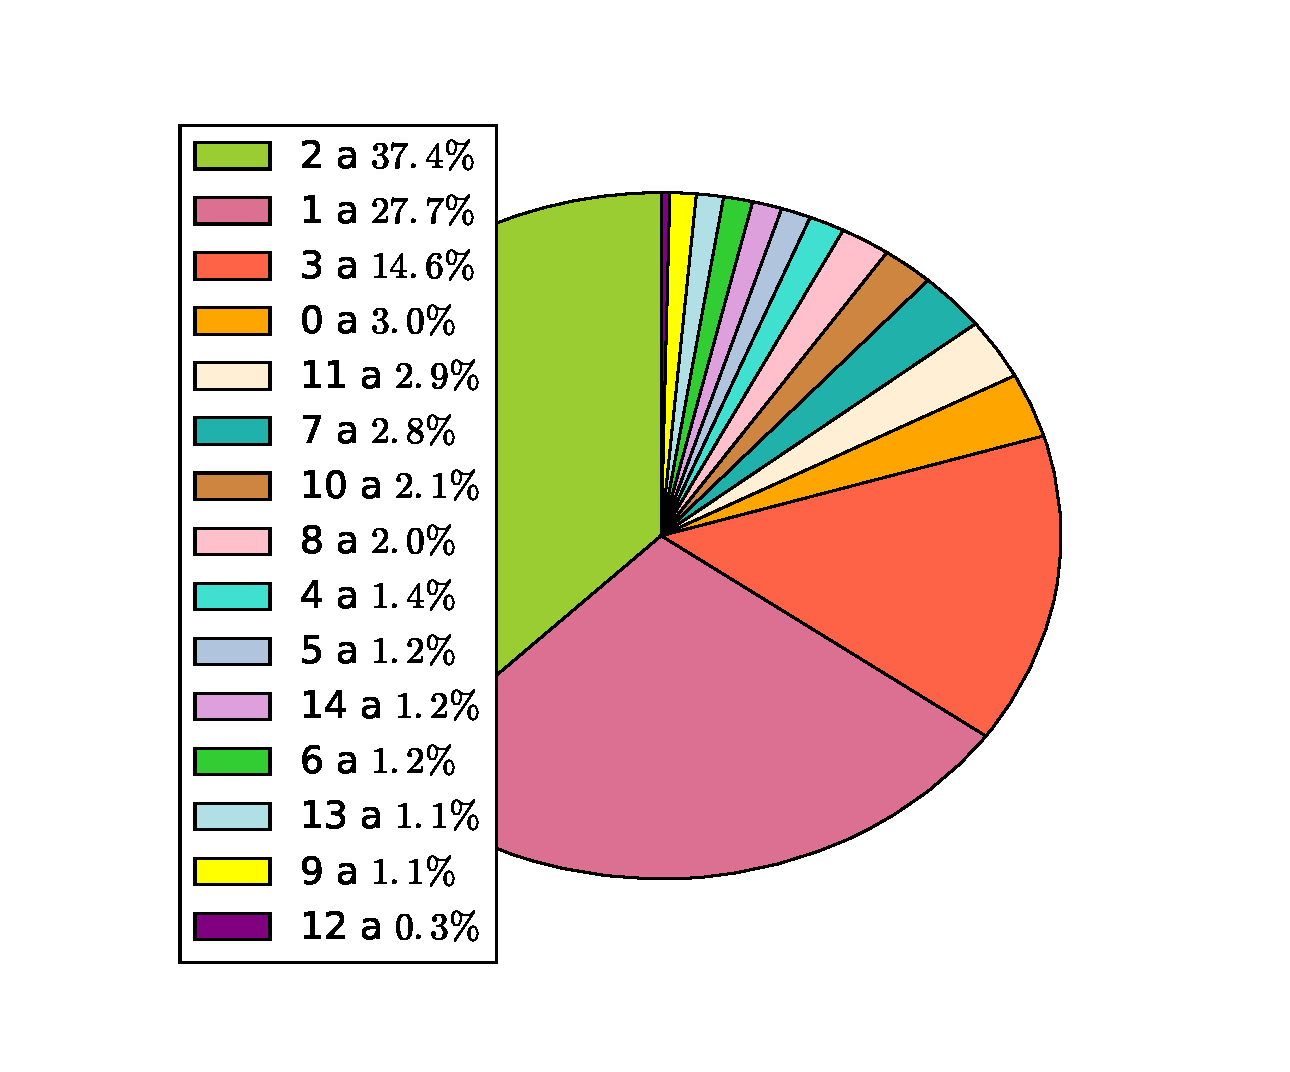
\includegraphics[width=10cm]{vanus_hoidja_sonad} }}
    \caption{lapse ja hoidja sõnade jaotumine kogu korpuses vanusegrupiti}
\end{figure}


\begin{figure}[H]
    \centering
    \subfloat[lapse sõnad]{{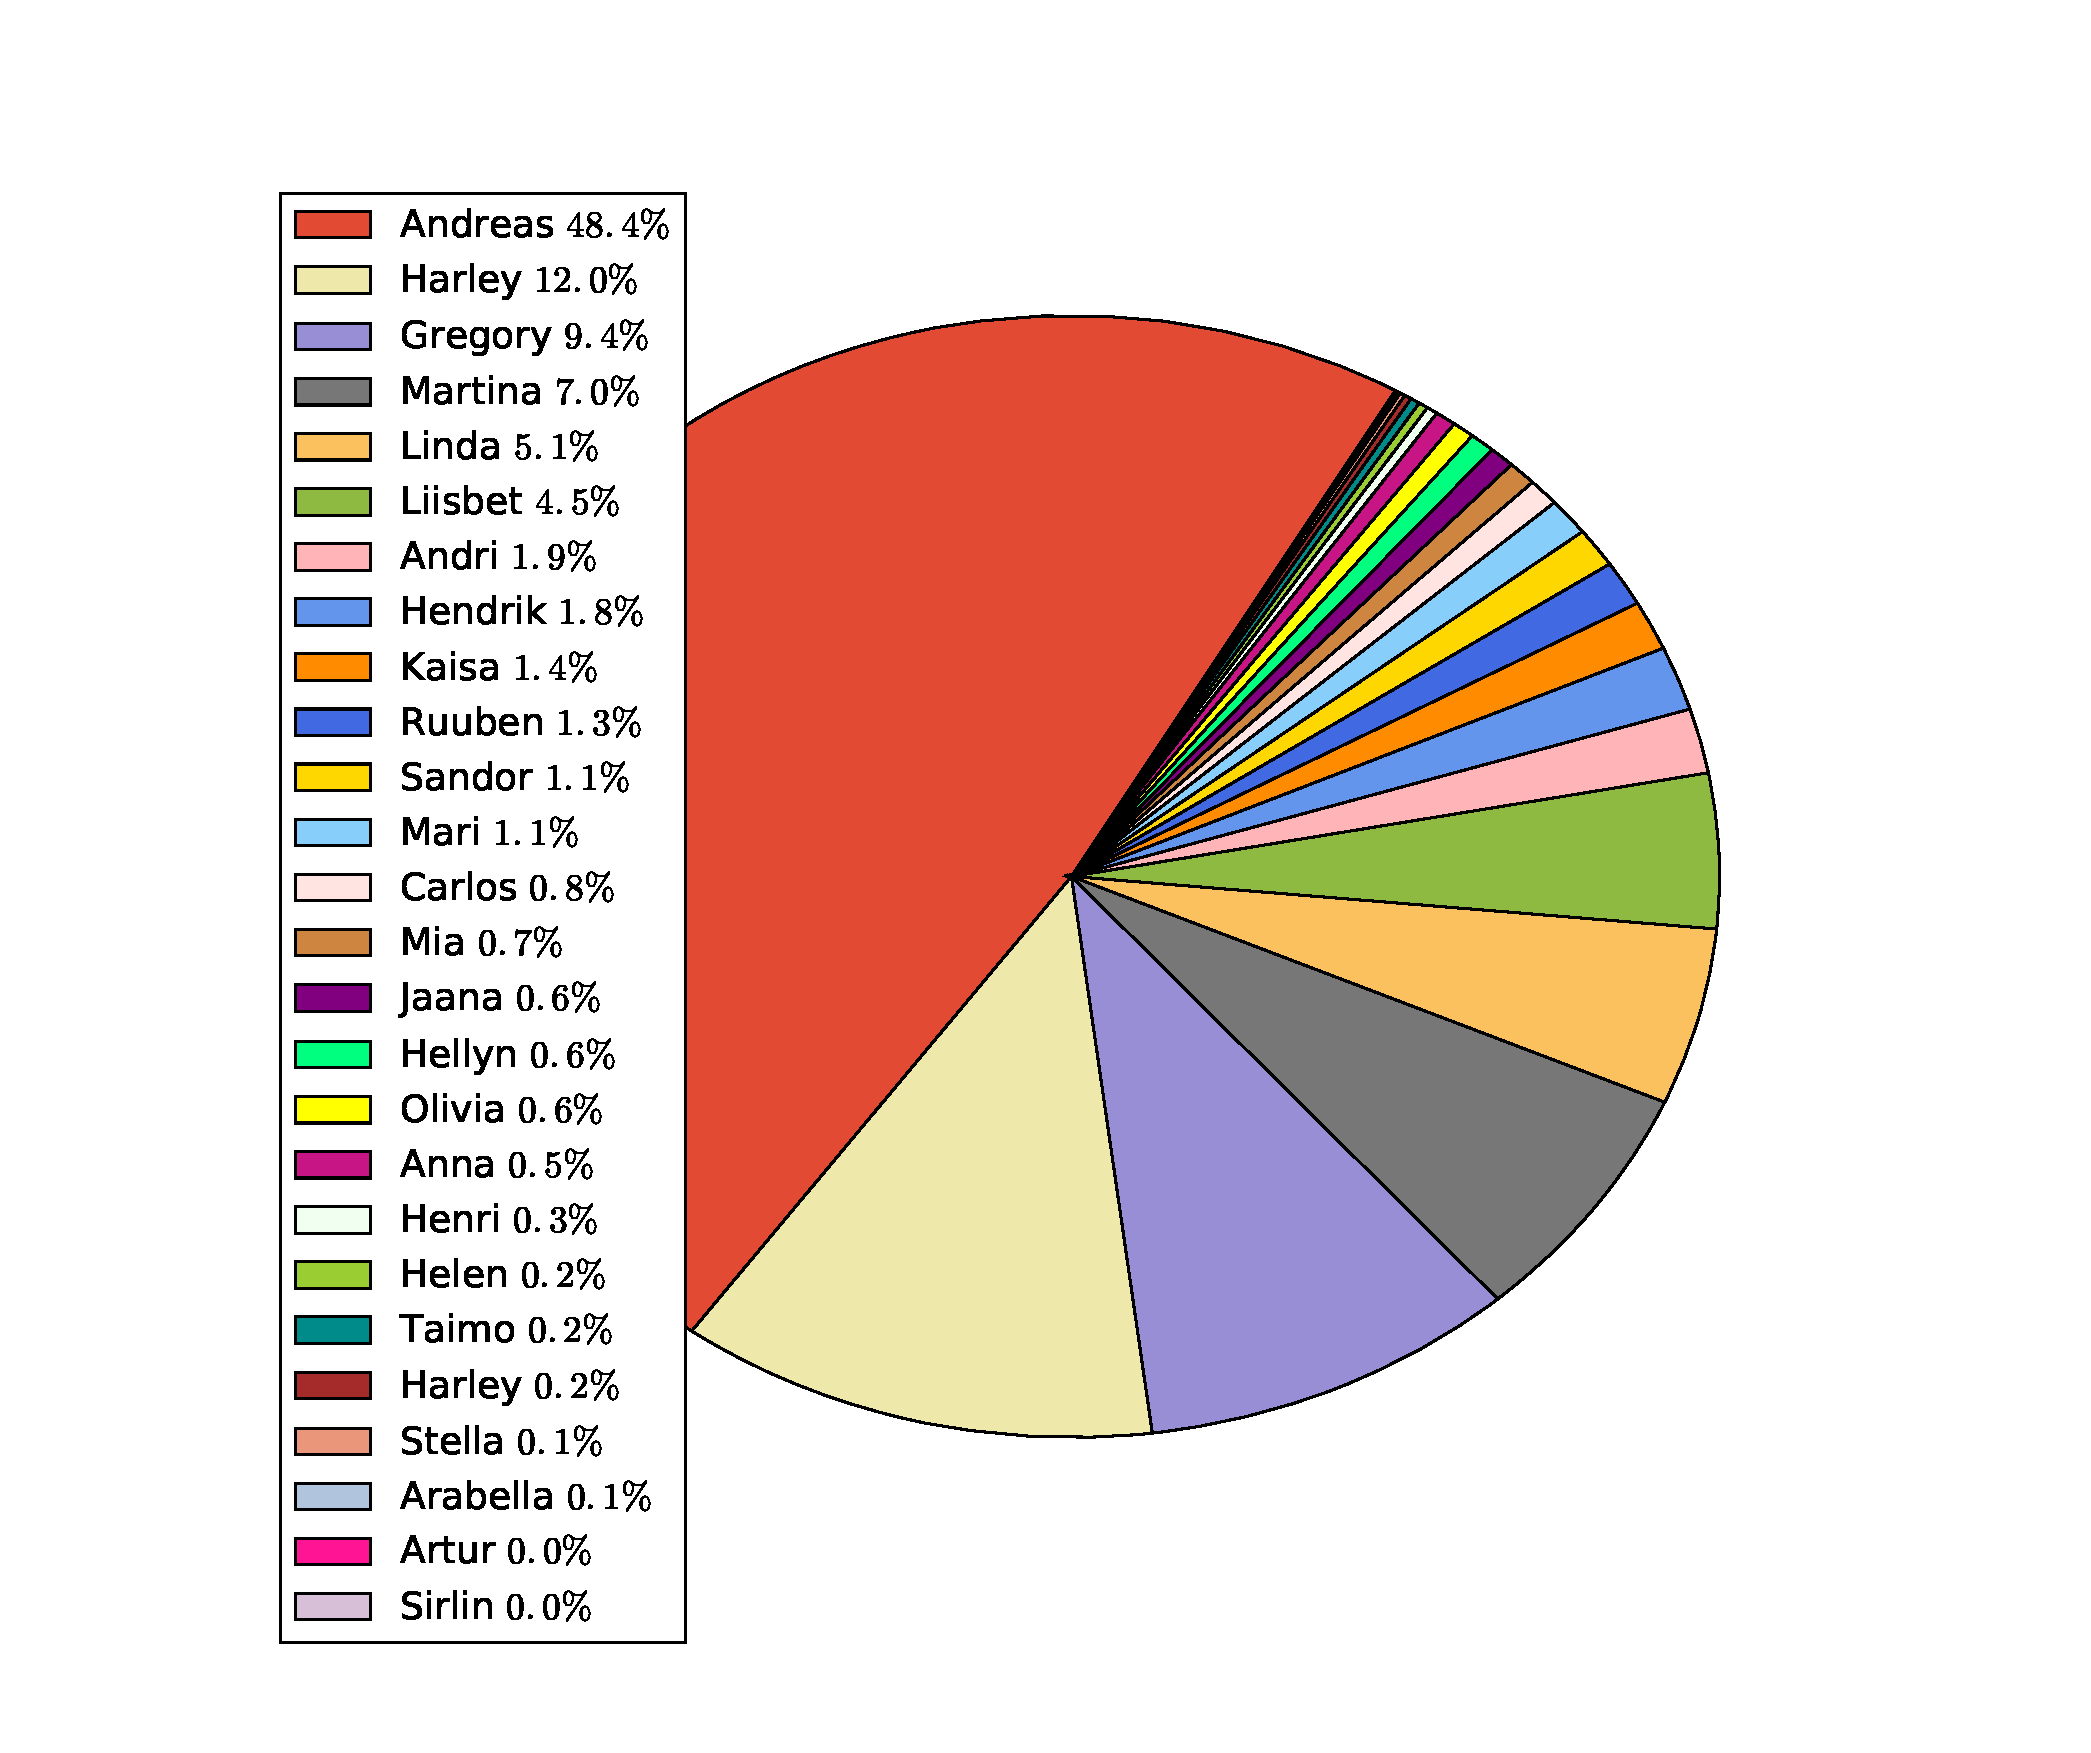
\includegraphics[width=10.5cm]{lapse_sonad_kogu_korpus} }}
    \qquad
    \subfloat[hoidja sõnad]{{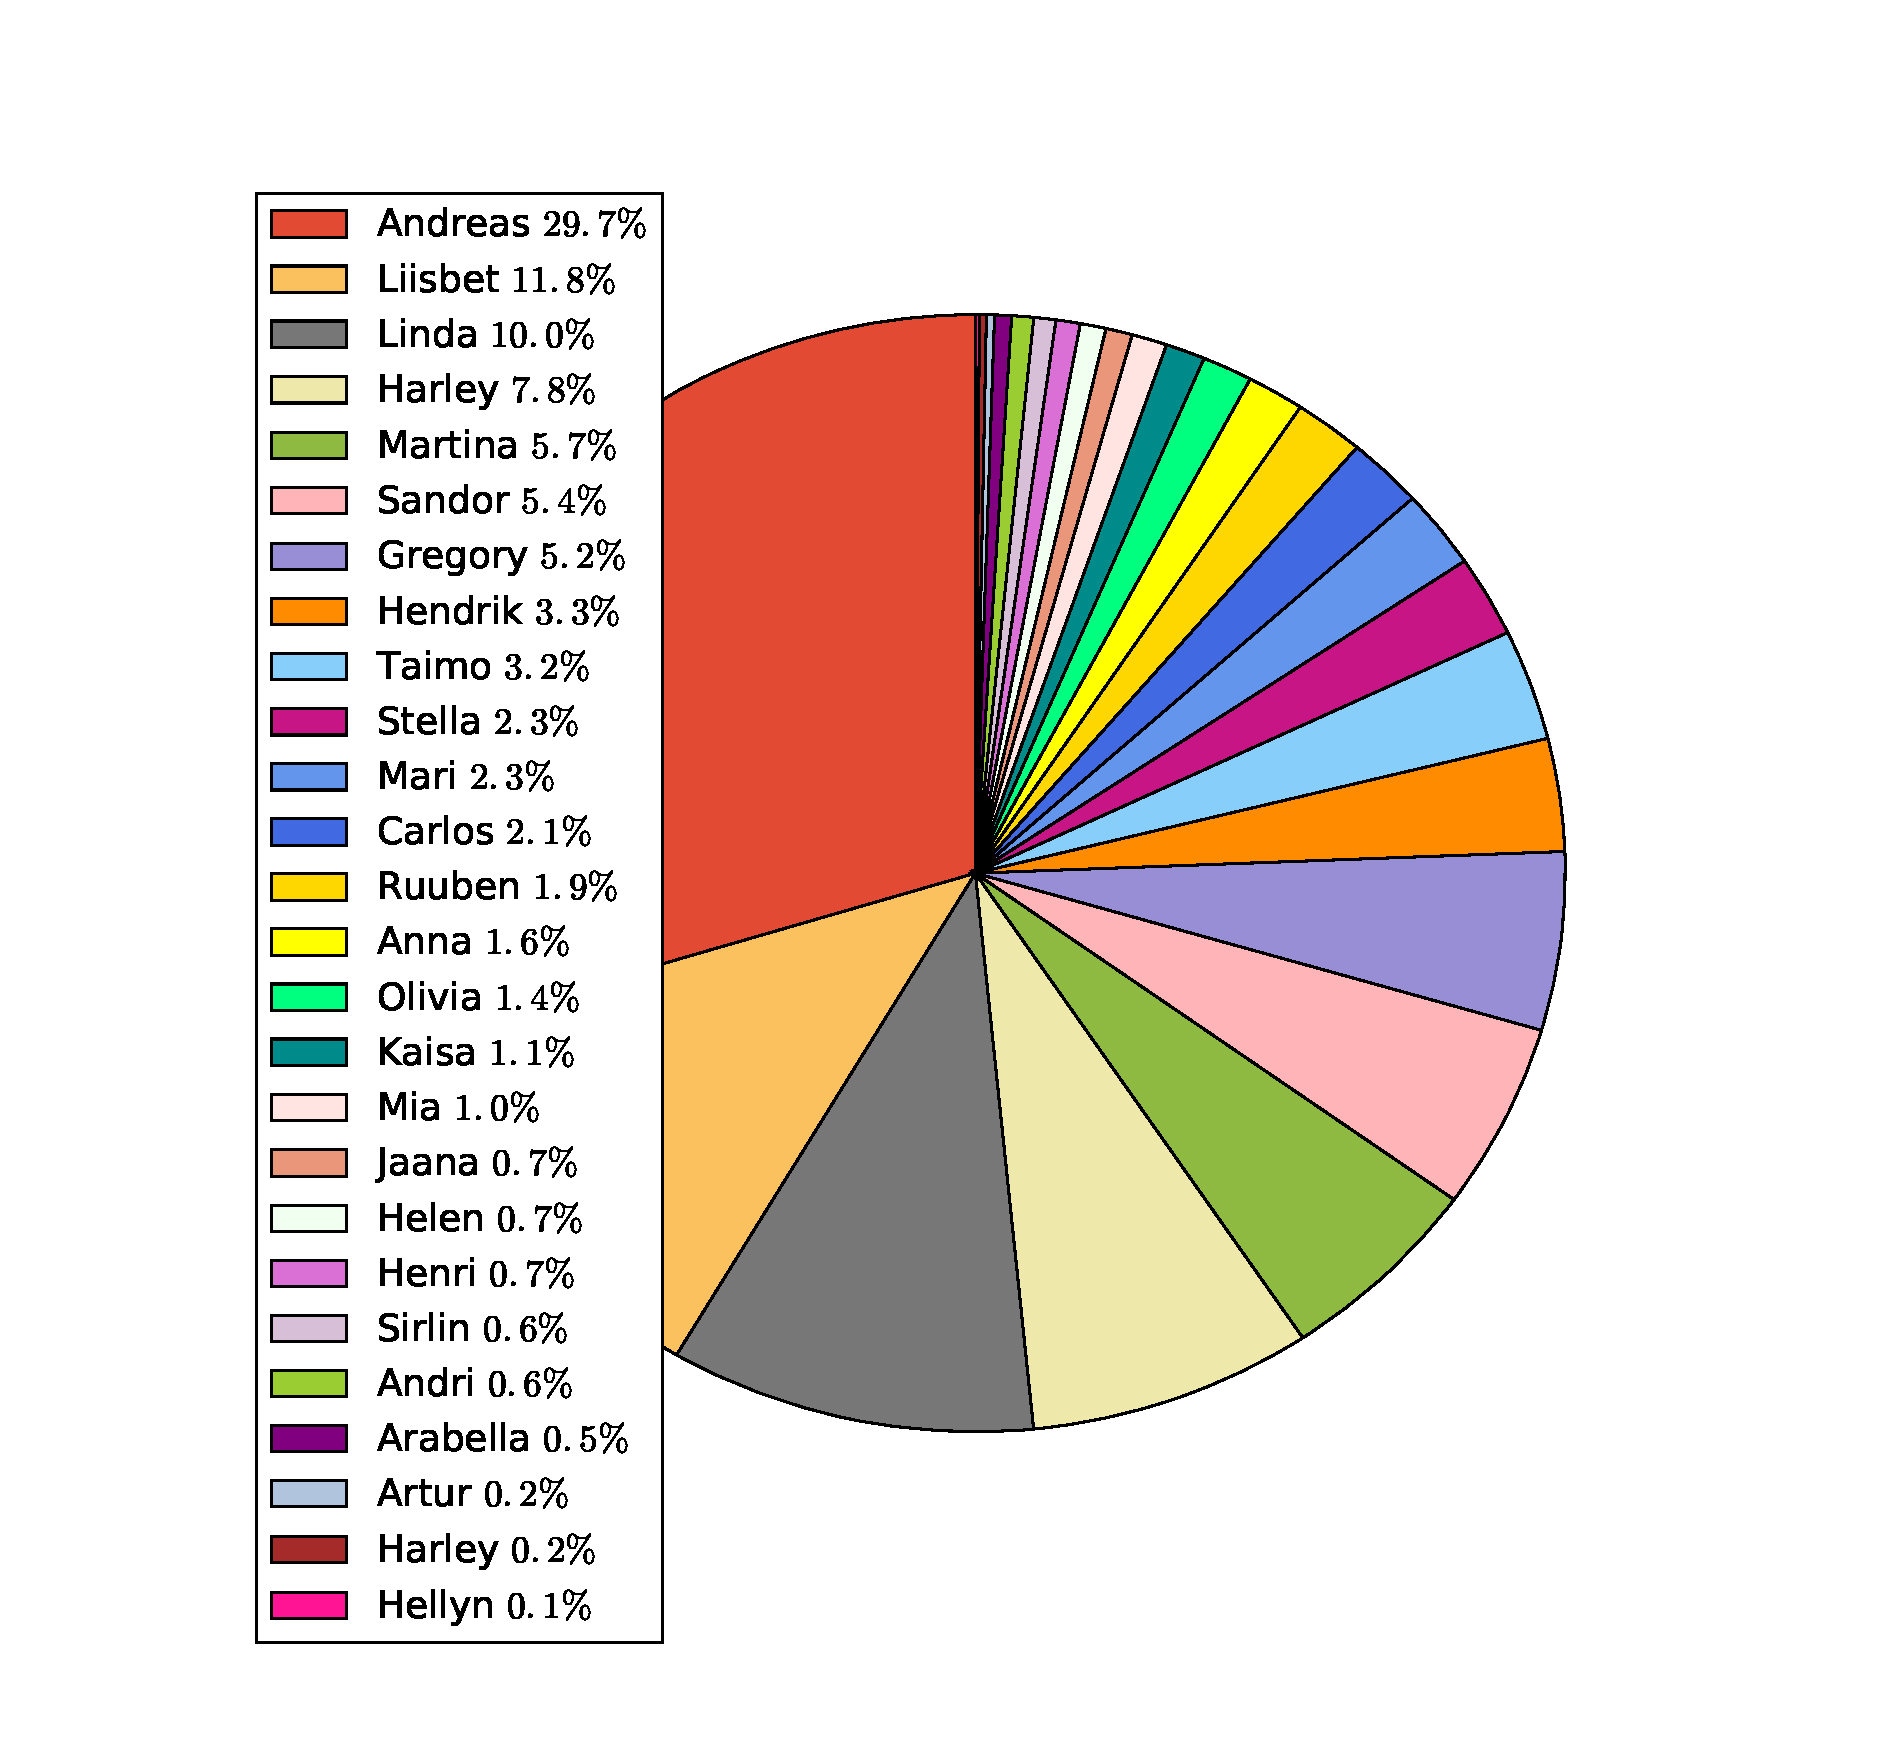
\includegraphics[width=10.5cm]{hoidja_sonad_kogu_korpuses} }}
    \caption{lapse ja hoidja sõnade jaotumine lapse järgi}
\end{figure}



Tabelis 2 on välja toodud see, kuidas jaotub lapse, hoidja ja nende kattuv sõnavara (ehk unikaalsete sõnade koguarv) igas alamkorpuses. Kõige ühtlasemalt jaotub lapse ja hoidja sõnavara Kapaneni korpuses (mõlema osakaal korpuses on 39\%) ja nende kattuv sõnavara on 22\%. Ka Kõrgesaare korpuses on jaotumine ühtlane -- lapse sõnavara moodustab 35\% ja hoidja sõnavara 36\%, seejuures kattuv sõnavara on 29\%. Vija ja Zuppingu korpusteski pole lapse ega hoidja sõnavaral suured erinevused (35\% ja 32\% ning 29\% ja 54\%). Kõige suuremad lahknevused on Beeki, Arguse ja Kohleri korpuses. Kohleri korpuses moodustab lapse sõnavara suurus kogu alamkorpuse sõnavarast 17\% ja hoidja sõnavara 58\%. Arguse korpuses moodustab lapse sõnavara kogu alamkorpuse sõnavarast 17\% ja hoidja sõnavara 69\%. Sõnavara jaotub kõige ebaühtlasemalt Beeki korpuses: lapse sõnavara moodustab 16\% ja hoidja sõnavara 78\%, nende ühine sõnavara alamkorpuse kogu sõnavarast on vaid 6\%. Kõige suurem ühise sõnavara \% on Vija alamkorpuses (33\%). Vija korpuse puhul on huvitav see, et see on ainus alamkorpus, kus lapse sõnavara on rikkam kui hoidja sõnavara.


\begin{table}[H]
\centering
\caption{lapse ja hoidja sõnavara jaotumine alamkorpustes}
\begin{tabular}{|l|c|c|c|c|}
\hline
korpus    & \multicolumn{1}{l|}{lapse sõnavara}               & \multicolumn{1}{l|}{hoidja sõnavara}              & \multicolumn{1}{l|}{kattuv sõnavara}            & \multicolumn{1}{l|}{KOKKU}                            \\ \hline\hline
Argus     & \begin{tabular}[c]{@{}c@{}}291\\ 17\%\end{tabular}  & \begin{tabular}[c]{@{}c@{}}1185\\ 69\%\end{tabular} & \begin{tabular}[c]{@{}c@{}}248\\ 14\%\end{tabular}  & \begin{tabular}[c]{@{}c@{}}1724\\ 100\%\end{tabular}  \\ \hline
Beek      & \begin{tabular}[c]{@{}c@{}}732\\ 16\%\end{tabular}  & \begin{tabular}[c]{@{}c@{}}3517\\ 78\%\end{tabular} & \begin{tabular}[c]{@{}c@{}}272\\ 6\%\end{tabular}   & \begin{tabular}[c]{@{}c@{}}4521\\ 100\%\end{tabular}  \\ \hline
Kapanen   & \begin{tabular}[c]{@{}c@{}}2661\\ 39\%\end{tabular} & \begin{tabular}[c]{@{}c@{}}2708\\ 39\%\end{tabular} & \begin{tabular}[c]{@{}c@{}}1533\\ 22\%\end{tabular} & \begin{tabular}[c]{@{}c@{}}6902\\ 100\%\end{tabular}  \\ \hline
Kohler    & \begin{tabular}[c]{@{}c@{}}817\\ 17\%\end{tabular}  & \begin{tabular}[c]{@{}c@{}}2700\\ 58\%\end{tabular} & \begin{tabular}[c]{@{}c@{}}1160\\ 25\%\end{tabular} & \begin{tabular}[c]{@{}c@{}}4677\\ 100\%\end{tabular}  \\ \hline
Kõrgesaar & \begin{tabular}[c]{@{}c@{}}5402\\ 35\%\end{tabular} & \begin{tabular}[c]{@{}c@{}}5665\\ 36\%\end{tabular} & \begin{tabular}[c]{@{}c@{}}4455\\ 29\%\end{tabular} & \begin{tabular}[c]{@{}c@{}}15522\\ 100\%\end{tabular} \\ \hline
Vija      & \begin{tabular}[c]{@{}c@{}}4834\\ 35\%\end{tabular} & \begin{tabular}[c]{@{}c@{}}4484\\ 32\%\end{tabular} & \begin{tabular}[c]{@{}c@{}}4643\\ 33\%\end{tabular} & \begin{tabular}[c]{@{}c@{}}13961\\ 100\%\end{tabular} \\ \hline
Zupping   & \begin{tabular}[c]{@{}c@{}}1615\\ 29\%\end{tabular} & \begin{tabular}[c]{@{}c@{}}3016\\ 54\%\end{tabular} & \begin{tabular}[c]{@{}c@{}}982\\ 17\%\end{tabular}  & \begin{tabular}[c]{@{}c@{}}5613\\ 100\%\end{tabular}  \\ \hline
\end{tabular}
\end{table}


Sõnavara kvantitatiivseks hindamiseks tuleb arvestada korpuse andmete kogumisviisi ja suurusega. Väikse andmestikuga korpused pole sõnavara ja harva esilduvate nähtuste uurimiseks kõige sobilikum viis, sest see võib viia valede järeldusteni. Tihe andmestik võimaldab jällegi saada rikkalikumat sõnavara, uurida lapse produktiivsust ja nähtusi, mis pole keeles nii sagedased. \citep{Tomasello} Kui vaadata Beeki, Arguse ja Zuppingu alamkorpustes lapse ja hoidja sõnavara kattumist, siis tekib küsimus, kas see vähene kattuvus tuleneb sellest, et lapsel ongi väike sõnavara, või sellest, et tegemist väikse korpusega? Alamkorpustes ei saa vanuse järgi lapse ja hoidja sõnavara kasvu adekvaatselt hinnata, sest tegu on väikeste andmestikega ja mõnes vanuses on last rohkem lindistatud. Lisaks tuleks ettevaatlikkusega suhtuda ka alamkorpuste võrdlemisse, sest iga korpus on koostatud erinevaid eesmärke ja viise silmas pidades.


\newpage

\section{Morfoloogiliselt märgendatud lapsekeele korpus}

\subsection{Tööprotsess}

Magistritöö eesmärk on luua morfoloogiliselt märgendatud eesti lapsekeele korpus, kuhu on koondatud kõik CHILDES-i eesti keele alamkorpused. Esialgne plaan oli konverteerida omalkäel kõik CHAT-failid XML-kujule, kuid sellega tekkisid mõningad tagasilöögid. Selleks, et faile XML-kujule konverteerida, oleks tarvis, et kõik alamkorpused oleksid ühtsel kujul transkribeeritud ja kodeeritud. Peatükis 3.2 tõin välja mõned näited sellest, kui ebajärjepidevalt on seda tehtud. Isegi, kui korpused oleksid olnud standardsel kujul, siis oleks konverteerimisskripti tegemine muutunud väga keeruliseks ja ülejõukäivaks ülesandeks. Põhjus seisneb selles, et CHILDES-i transkriptsioonisüsteemis on väga suur ja lai valik kodeeringuid, mida on paraku ühel inimesel raske hallata. Näide (5) illustreerib seda, kuidas juba ühes lühikeses transkriptsiooni lõigus võib kodeeringute kasutus olla väga mitmekesine (kodeeringu seletus paikneb lausungi järel).

(5)
\begin{description}
    \item*CHI:   see kifiir \textbf{[:} kefiir\textbf{]} . | \emph{asendus}
    \item*MOT:   kus sa $\pmb{+/}$. | \emph{vahele segamine}
    \item*CHI:   $\pmb{+<}$ \textbf{(}h\textbf{)}akkas põlema . | \emph{pealerääkimine}, \emph{mittetäielik sõna}
    \item*MOT:   see ei ole kefiir ju .
    \item*CHI:   kefiir . $\pmb{[+}$ sr\textbf{]} | üleskirjutaja poolt defineeritud \emph{postcode}
    \item*MOT:   see on piim .
    \item*FAT:   mis see kook teeb ?
    \item*FAT:   tuleb ära panna $\pmb{[=}$ visata\textbf{]} või ? | \emph{seletus, tähendus}
    \item*MOT:   mina ei tea , vist jah .
    \item*CHI:   kuidas emme küpsetab saia , lihat\textbf{@n} \textbf{[*]} . | \emph{üleüldistamine}, \emph{vea markeerimine}
    \item\%err:   lihat=liha \$MOR
    \item*FAT:   saia ei ei küpseta .
    \item*FAT:   kartulit küpsetame , \textbf{(.)} ahjus . | \emph{paus}
    \item*CHI:   $\pmb{+<}$ saia . | \emph{pealerääkimine}
    \item*CHI:   lihat\textbf{@n} \textbf{[*]} . $\pmb{[+}$ \textbf{sr]} | \emph{postcode}
    \item\%err:   lihat=liha \$MOR
    \item*FAT:   liha ka jah .
    \item*CHI:   lihat\textbf{@n} \textbf{[*]} . $\pmb{[+}$ \textbf{sr]} | \emph{üleüldistamine}, \emph{vea markeerimine}, \emph{postcode}
    \item\%err:   lihat=liha \$MOR
    \item\%act:   MOT koorib sibulat
    \item...
    \item*CHI:   Atu \textbf{[:} Andreas\textbf{]} sõi $\pmb{+...}$ | \emph{asendus}, \emph{kõrvalekalle}
    \item*CHI:   $\pmb{+}$\textbf{"} a . | \emph{lausung jutumärkides}
    \item...
    \item*CHI:   käpad \textbf{(}h\textbf{)}aige \textbf{[*]} \textbf{[$\pmb{/]}$} käpad \textbf{(}h\textbf{)}aige \textbf{[*]} . | \emph{mittetäielik sõna}, \emph{vea markeerimine}, \emph{kordus}
    \item (Vija; 20018.cha)
\end{description}

\hfill

On arusaadav, et iga uurija transkribeerib ja kodeerib lindistusi lähtuvalt enda eesmärkidest. Ühelt poolt on hea, et transkriptsioonisüsteem on niivõrd detailne, kuid teisalt võib selles orienteerumine vägagi raskeks osutuda. Kuna sellise konverteerimisskripti kirjutamise töömaht oleks selle magistritöö kirjutamise jaoks liiga töömahukaks osutunud, siis tuli leida uus lahendus. Korpuse tegemiseks vajalik keelematerjal pärineb samuti CHILDES-i andmebaasist, kuid need on juba eelnevalt CHAT-kujult XML-kujule konverteeritud failid. Aga kuna selle töö eesmärk on luua morfoloogiliselt märgendatud korpus, siis tuli nendele XML-failidele ka lisada morfoloogiline tasand, mida neis failides ei ole. Kuna kõik CHILDES-i korpused on kirjeldatud oma XML-skeema (\emph{Talkbank}) järgi, siis tuli lähemalt tutvuda Talkbanki XML-skeema süntaksiga.

\subsubsection{\emph{Talkbank}i skeema}

Joonisel 6 on kujutatud minu töö seisukohalt olulisimad skeema elemendid.

\begin{figure}[H]
    \centering
    \includegraphics[width=10cm]{tag_elemendid}
    \caption{Talkbanki skeema elemendid}
\end{figure}

Talkbanki skeema juurelement on \emph{<CHAT>}, mille alluvad on \emph{<comment>}, \emph{<Participants>} ja \emph{<u>}. Elemendi \emph{<Participants>} alluv on \emph{<participant>}. \emph{<participant>} elemendis peitub metainfo lindistuse osalejate kohta (kõneleja ID, nimi, roll, keel, vanus ja sugu). Element \emph{<comment>} talletab metainfot lindistuse konteksti kohta (nt koht, kuupäev, lindistuse algus ja lõpp jne).

Näide (6) (Argus; hend10.xml)
\begin{lstlisting}
  <Participants>
    <participant
      id="CHI"
      name="Hendrik"
      role="Target_Child"
      language="est"
      age="P2Y2M6D"/>
    <participant
      id="EMA"
      role="Mother"
      language="est"/>
  </Participants>
  <comment type="Date">02-JUN-1997</comment>
\end{lstlisting}

Element \emph{<u>} tähistab kõneleja lausungit, selle kohustuslikeks atribuutideks on kõneleja ID ja lausungi järjekorra ID. \emph{<u>}-elemendil on palju alluvaid, aga selle töö juures osutusid olulisimateks \emph{<w>} ja \emph{<g>}. Element \emph{<w>} tähistab sõna ja \emph{<g>} sõnade gruppi. \emph{<g>} alluvaks võib olla tema ise või \emph{<w>}. Elemendi \emph{<w>} alluvaks võib olla \emph{<replacement>}. See element tähistab neid üksuseid, mida CHILDES-i konventsioonide järgi kodeeritakse [: text] abil, vt näide (7) (vt ka näide (5) kifiir [: kefiir]).

\hfill

Näide (7) (Kohler; car030900.xml)
\begin{lstlisting}
<u who='CHI' uID='u58'>
  <w>ehitame</w>
  <w>
      galaasi
      <replacement>
          <w>garaazhi</w>
      </replacement>
  </w>
  <t type='p'></t>
</u>
\end{lstlisting}

Morfoloogilise tasandi lisamine algab elemendiga \emph{<mor>}, mille alluv on \emph{<mw>} ehk \emph{morphemicWordType}. See jaguneb elemendiks \emph{<pos>} ja \emph{<stem>}. \emph{<pos>} tähistab sõnaliiki (ingl k. \emph{part of speech}). Selle alluvaks on \emph{<c>} ehk sõna morfoloogiline kategooria, mille sisuks on mittetühi string. Element \emph{<stem>} tähistab sõnatüve, mille sisuks on samuti mittetühi string.

\subsubsection{Morfoloogilise info lisamine}

\begin{figure}[H]
    \centering
    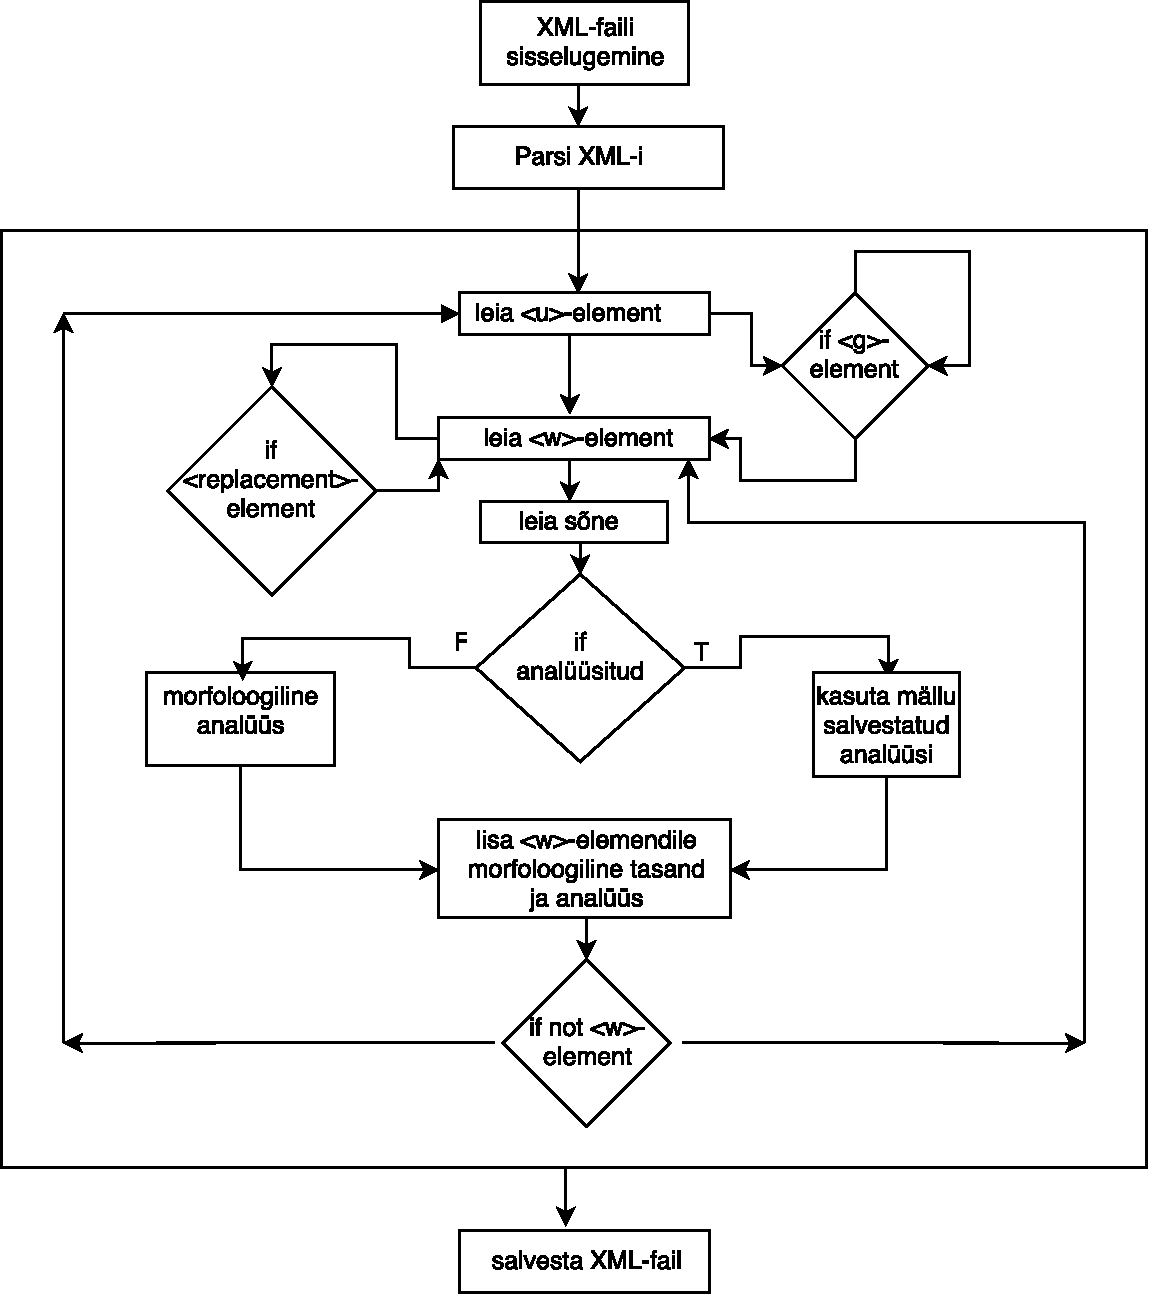
\includegraphics[width=12cm]{toovoog}
    \caption{Töövoog}
\end{figure}


Programmi kirjutamiseks on kasutatud Python 3.4 versiooni. Töövoog (vt joonis 7) on jaotatud 4 suuremaks osaks: XML-failide sisselugemine, faili parsimine, töötlemine ja modifitseeritud XML-faili salvestamine. Faili parsimiseks kasutan Pythoni moodulit \emph{ElementTree}, mis võimaldab lugeda ja genereerida XML hierarhiat. Parsimise käigus pannakse paika XML-faili juurelement ja sellele alluvad elemendid. Töötluse käigus navigeeritakse esmalt iga vestlusest osavõtja lausungi juurde. Seejärel leitakse kõik sõned ehk \emph{<w>}-elemendid. Juhul kui \emph{<w>}-elemendi alluv on element \emph{<replacement>}, siis uueks sõneks määratakse \emph{<replacement>}-elemendi \emph{<w>}-element.

Kui lausungi sõne on leitud, siis tehakse sõnele morfoloogiline analüüs. Morfoloogilise analüsaatorina kasutatakse \emph{etanat}. Sõne analüüs salvestatakse mällu. Kui analüsaator saab sisendiks seni nägemata sõne (ehk mida mälus ei eksisteeri), siis tehakse sellele morfoloogiline analüüs. Põhjus seisneb programmi optimeerimises: morfoloogilise analüsaatori kutsumine iga sõne juures on üsna kulukas protsess. Seejärel lisatakse igale sõnele morfoloogiline tasand. Programm genereerib kirjutatud koodis järk-järgult puu elemendid ning morfoloogilisele tasandile jõudes hakkab sõne analüüse neile vastavatesse elementidesse lisama (vt joonis 7 ja näide (8)). Juhul kui sõne analüüse on rohkem kui üks, siis igale analüüsile genereeritakse uuesti morfoloogilise taseme elemendid. Samme korratakse seni, kuni jõutakse viimase lausungini ja lõpptulemus salvestatakse modifitseeritud XML-faili.

Näide (8) (Vija; 11120.xml)
\begin{lstlisting}
  <u uID="u7" who="CHI">
    <w>tuli
        <mor type="mor">
            <mw>
                <pos><c>_V_ Pers Prt Ind Sg3 Aff</c></pos>
                <stem>tule+i</stem>
            </mw>
        </mor>
        <mor type="mor">
            <mw>
                <pos><c>_S_ Sg Nom</c></pos>
                <stem>tuli+0</stem>
            </mw>
        </mor>
    </w>
    ...
\end{lstlisting}

\subsection{Morfoloogilise märgenduse hindamine}

Analüüsisin korpuseid morfoloogilist analüsaatorit kohandamata. Analüüsimisel ei teostatud oletamist ega ühestamist. Selle alapeatüki eesmärk on anda ülevaade sellest, kuidas jaotuvad analüüsi saanud ja tundmatuks jäänud sõnad igas vanuserühmas alamkorpuse kaupa.


\begin{table}[H]
\centering
\caption{Kõrgesaare korpus}
\resizebox{\textwidth}{!}{
\begin{tabular}{|l|c|c|c|c|c|c|}
\hline
vanus                  & \multicolumn{3}{c|}{lapse sõnad}                                                                                                                                                                                     & \multicolumn{3}{c|}{hoidja sõnad}                                                                                                                                                                                    \\ \hline
                       & \multicolumn{1}{l|}{analüüsitud}                                      & \multicolumn{1}{l|}{tundmatud}                                      & \multicolumn{1}{l|}{KOKKU}                                             & \multicolumn{1}{l|}{analüüsitud}                                      & \multicolumn{1}{l|}{tundmatud}                                      & \multicolumn{1}{l|}{KOKKU}                                             \\ \hline\hline
\multirow{2}{*}{1}     & \multirow{2}{*}{\begin{tabular}[c]{@{}c@{}}515\\ 47\%\end{tabular}}   & \multirow{2}{*}{\begin{tabular}[c]{@{}c@{}}575\\ 53\%\end{tabular}} & \multirow{2}{*}{\begin{tabular}[c]{@{}c@{}}1090\\ 100\%\end{tabular}}  & \multirow{2}{*}{\begin{tabular}[c]{@{}c@{}}11033\\ 93\%\end{tabular}} & \multirow{2}{*}{\begin{tabular}[c]{@{}c@{}}838\\ 7\%\end{tabular}}  & \multirow{2}{*}{\begin{tabular}[c]{@{}c@{}}11871\\ 100\%\end{tabular}} \\
                       &                                                                       &                                                                     &                                                                        &                                                                       &                                                                     &                                                                        \\ \hline
\multirow{2}{*}{2}     & \multirow{2}{*}{\begin{tabular}[c]{@{}c@{}}3208\\ 80\%\end{tabular}}  & \multirow{2}{*}{\begin{tabular}[c]{@{}c@{}}818\\ 20\%\end{tabular}} & \multirow{2}{*}{\begin{tabular}[c]{@{}c@{}}4026\\ 100\%\end{tabular}}  & \multirow{2}{*}{\begin{tabular}[c]{@{}c@{}}10030\\ 95\%\end{tabular}} & \multirow{2}{*}{\begin{tabular}[c]{@{}c@{}}534\\ 5\%\end{tabular}}  & \multirow{2}{*}{\begin{tabular}[c]{@{}c@{}}10564\\ 100\%\end{tabular}} \\
                       &                                                                       &                                                                     &                                                                        &                                                                       &                                                                     &                                                                        \\ \hline
\multirow{2}{*}{3}     & \multirow{2}{*}{\begin{tabular}[c]{@{}c@{}}2292\\ 90\%\end{tabular}}  & \multirow{2}{*}{\begin{tabular}[c]{@{}c@{}}242\\ 10\%\end{tabular}} & \multirow{2}{*}{\begin{tabular}[c]{@{}c@{}}2534\\ 100\%\end{tabular}}  & \multirow{2}{*}{\begin{tabular}[c]{@{}c@{}}5232\\ 94\%\end{tabular}}  & \multirow{2}{*}{\begin{tabular}[c]{@{}c@{}}319\\ 6\%\end{tabular}}  & \multirow{2}{*}{\begin{tabular}[c]{@{}c@{}}5551\\ 100\%\end{tabular}}  \\
                       &                                                                       &                                                                     &                                                                        &                                                                       &                                                                     &                                                                        \\ \hline
\multirow{2}{*}{4}     & \multirow{2}{*}{\begin{tabular}[c]{@{}c@{}}1439\\ 81\%\end{tabular}}  & \multirow{2}{*}{\begin{tabular}[c]{@{}c@{}}330\\ 19\%\end{tabular}} & \multirow{2}{*}{\begin{tabular}[c]{@{}c@{}}1769\\ 100\%\end{tabular}}  & \multirow{2}{*}{\begin{tabular}[c]{@{}c@{}}3929\\ 95\%\end{tabular}}  & \multirow{2}{*}{\begin{tabular}[c]{@{}c@{}}210\\ 5\%\end{tabular}}  & \multirow{2}{*}{\begin{tabular}[c]{@{}c@{}}4139\\ 100\%\end{tabular}}  \\
                       &                                                                       &                                                                     &                                                                        &                                                                       &                                                                     &                                                                        \\ \hline
\multirow{2}{*}{5}     & \multirow{2}{*}{\begin{tabular}[c]{@{}c@{}}2947\\ 91\%\end{tabular}}  & \multirow{2}{*}{\begin{tabular}[c]{@{}c@{}}309\\ 9\%\end{tabular}}  & \multirow{2}{*}{\begin{tabular}[c]{@{}c@{}}3256\\ 100\%\end{tabular}}  & \multirow{2}{*}{\begin{tabular}[c]{@{}c@{}}4531\\ 97\%\end{tabular}}  & \multirow{2}{*}{\begin{tabular}[c]{@{}c@{}}159\\ 3\%\end{tabular}}  & \multirow{2}{*}{\begin{tabular}[c]{@{}c@{}}4690\\ 100\%\end{tabular}}  \\
                       &                                                                       &                                                                     &                                                                        &                                                                       &                                                                     &                                                                        \\ \hline
\multirow{2}{*}{6}     & \multirow{2}{*}{\begin{tabular}[c]{@{}c@{}}3222\\ 94\%\end{tabular}}  & \multirow{2}{*}{\begin{tabular}[c]{@{}c@{}}213\\ 6\%\end{tabular}}  & \multirow{2}{*}{\begin{tabular}[c]{@{}c@{}}3435\\ 100\%\end{tabular}}  & \multirow{2}{*}{\begin{tabular}[c]{@{}c@{}}4435\\ 97\%\end{tabular}}  & \multirow{2}{*}{\begin{tabular}[c]{@{}c@{}}135\\ 3\%\end{tabular}}  & \multirow{2}{*}{\begin{tabular}[c]{@{}c@{}}4570\\ 100\%\end{tabular}}  \\
                       &                                                                       &                                                                     &                                                                        &                                                                       &                                                                     &                                                                        \\ \hline
\multirow{2}{*}{7}     & \multirow{2}{*}{\begin{tabular}[c]{@{}c@{}}7572\\ 94\%\end{tabular}}  & \multirow{2}{*}{\begin{tabular}[c]{@{}c@{}}518\\ 6\%\end{tabular}}  & \multirow{2}{*}{\begin{tabular}[c]{@{}c@{}}8090\\ 100\%\end{tabular}}  & \multirow{2}{*}{\begin{tabular}[c]{@{}c@{}}10489\\ 97\%\end{tabular}} & \multirow{2}{*}{\begin{tabular}[c]{@{}c@{}}278\\ 3\%\end{tabular}}  & \multirow{2}{*}{\begin{tabular}[c]{@{}c@{}}10767\\ 100\%\end{tabular}} \\
                       &                                                                       &                                                                     &                                                                        &                                                                       &                                                                     &                                                                        \\ \hline
\multirow{2}{*}{8}     & \multirow{2}{*}{\begin{tabular}[c]{@{}c@{}}5878\\ 94\%\end{tabular}}  & \multirow{2}{*}{\begin{tabular}[c]{@{}c@{}}400\\ 6\%\end{tabular}}  & \multirow{2}{*}{\begin{tabular}[c]{@{}c@{}}6278\\ 100\%\end{tabular}}  & \multirow{2}{*}{\begin{tabular}[c]{@{}c@{}}7522\\ 95\%\end{tabular}}  & \multirow{2}{*}{\begin{tabular}[c]{@{}c@{}}367\\ 5\%\end{tabular}}  & \multirow{2}{*}{\begin{tabular}[c]{@{}c@{}}7889\\ 100\%\end{tabular}}  \\
                       &                                                                       &                                                                     &                                                                        &                                                                       &                                                                     &                                                                        \\ \hline
\multirow{2}{*}{9}     & \multirow{2}{*}{\begin{tabular}[c]{@{}c@{}}3658\\ 93\%\end{tabular}}  & \multirow{2}{*}{\begin{tabular}[c]{@{}c@{}}269\\ 7\%\end{tabular}}  & \multirow{2}{*}{\begin{tabular}[c]{@{}c@{}}3927\\ 100\%\end{tabular}}  & \multirow{2}{*}{\begin{tabular}[c]{@{}c@{}}3879\\ 94\%\end{tabular}}  & \multirow{2}{*}{\begin{tabular}[c]{@{}c@{}}246\\ 6\%\end{tabular}}  & \multirow{2}{*}{\begin{tabular}[c]{@{}c@{}}4125\\ 100\%\end{tabular}}  \\
                       &                                                                       &                                                                     &                                                                        &                                                                       &                                                                     &                                                                        \\ \hline
\multirow{2}{*}{10}    & \multirow{2}{*}{\begin{tabular}[c]{@{}c@{}}7536\\ 94\%\end{tabular}}  & \multirow{2}{*}{\begin{tabular}[c]{@{}c@{}}518\\ 6\%\end{tabular}}  & \multirow{2}{*}{\begin{tabular}[c]{@{}c@{}}8054\\ 100\%\end{tabular}}  & \multirow{2}{*}{\begin{tabular}[c]{@{}c@{}}7717\\ 95\%\end{tabular}}  & \multirow{2}{*}{\begin{tabular}[c]{@{}c@{}}378\\ 5\%\end{tabular}}  & \multirow{2}{*}{\begin{tabular}[c]{@{}c@{}}8095\\ 100\%\end{tabular}}  \\
                       &                                                                       &                                                                     &                                                                        &                                                                       &                                                                     &                                                                        \\ \hline
\multirow{2}{*}{11}    & \multirow{2}{*}{\begin{tabular}[c]{@{}c@{}}11240\\ 93\%\end{tabular}} & \multirow{2}{*}{\begin{tabular}[c]{@{}c@{}}851\\ 7\%\end{tabular}}  & \multirow{2}{*}{\begin{tabular}[c]{@{}c@{}}12091\\ 100\%\end{tabular}} & \multirow{2}{*}{\begin{tabular}[c]{@{}c@{}}10762\\ 96\%\end{tabular}} & \multirow{2}{*}{\begin{tabular}[c]{@{}c@{}}399\\ 4\%\end{tabular}}  & \multirow{2}{*}{\begin{tabular}[c]{@{}c@{}}11161\\ 100\%\end{tabular}} \\
                       &                                                                       &                                                                     &                                                                        &                                                                       &                                                                     &                                                                        \\ \hline
\multirow{2}{*}{12}    & \multirow{2}{*}{\begin{tabular}[c]{@{}c@{}}1847\\ 92\%\end{tabular}}  & \multirow{2}{*}{\begin{tabular}[c]{@{}c@{}}156\\ 8\%\end{tabular}}  & \multirow{2}{*}{\begin{tabular}[c]{@{}c@{}}2003\\ 100\%\end{tabular}}  & \multirow{2}{*}{\begin{tabular}[c]{@{}c@{}}1274\\ 95\%\end{tabular}}  & \multirow{2}{*}{\begin{tabular}[c]{@{}c@{}}70\\ 5\%\end{tabular}}   & \multirow{2}{*}{\begin{tabular}[c]{@{}c@{}}1344\\ 100\%\end{tabular}}  \\
                       &                                                                       &                                                                     &                                                                        &                                                                       &                                                                     &                                                                        \\ \hline
\multirow{2}{*}{13}    & \multirow{2}{*}{\begin{tabular}[c]{@{}c@{}}3798\\ 89\%\end{tabular}}  & \multirow{2}{*}{\begin{tabular}[c]{@{}c@{}}492\\ 11\%\end{tabular}} & \multirow{2}{*}{\begin{tabular}[c]{@{}c@{}}4290\\ 100\%\end{tabular}}  & \multirow{2}{*}{\begin{tabular}[c]{@{}c@{}}4062\\ 95\%\end{tabular}}  & \multirow{2}{*}{\begin{tabular}[c]{@{}c@{}}199\\ 5\%\end{tabular}}  & \multirow{2}{*}{\begin{tabular}[c]{@{}c@{}}4261\\ 100\%\end{tabular}}  \\
                       &                                                                       &                                                                     &                                                                        &                                                                       &                                                                     &                                                                        \\ \hline
\multirow{2}{*}{14}    & \multirow{2}{*}{\begin{tabular}[c]{@{}c@{}}4525\\ 91\%\end{tabular}}  & \multirow{2}{*}{\begin{tabular}[c]{@{}c@{}}451\\ 9\%\end{tabular}}  & \multirow{2}{*}{\begin{tabular}[c]{@{}c@{}}4976\\ 100\%\end{tabular}}  & \multirow{2}{*}{\begin{tabular}[c]{@{}c@{}}4318\\ 93\%\end{tabular}}  & \multirow{2}{*}{\begin{tabular}[c]{@{}c@{}}347\\ 7\%\end{tabular}}  & \multirow{2}{*}{\begin{tabular}[c]{@{}c@{}}4665\\ 100\%\end{tabular}}  \\
                       &                                                                       &                                                                     &                                                                        &                                                                       &                                                                     &                                                                        \\ \hline\hline
\multirow{2}{*}{KOKKU} & \multirow{2}{*}{\begin{tabular}[c]{@{}c@{}}59677\\ 91\%\end{tabular}} & \multirow{2}{*}{\begin{tabular}[c]{@{}c@{}}6142\\ 9\%\end{tabular}} & \multirow{2}{*}{\begin{tabular}[c]{@{}c@{}}65819\\ 100\%\end{tabular}} & \multirow{2}{*}{\begin{tabular}[c]{@{}c@{}}89213\\ 95\%\end{tabular}} & \multirow{2}{*}{\begin{tabular}[c]{@{}c@{}}4479\\ 5\%\end{tabular}} & \multirow{2}{*}{\begin{tabular}[c]{@{}c@{}}93692\\ 100\%\end{tabular}} \\
                       &                                                                       &                                                                     &                                                                        &                                                                       &                                                                     &                                                                        \\ \hline
\end{tabular}}
\end{table}


\begin{table}[H]
\centering
\caption{Kapaneni korpus}
\resizebox{\textwidth}{!}{
\begin{tabular}{|l|c|c|c|c|c|c|}
\hline
vanus                  & \multicolumn{3}{c|}{lapse sõnad}                                                                                                                                                                                      & \multicolumn{3}{c|}{hoidja sõnad}                                                                                                                                                                                    \\ \hline
                       & \multicolumn{1}{l|}{analüüsitud}                                      & \multicolumn{1}{l|}{tundmatud}                                       & \multicolumn{1}{l|}{KOKKU}                                             & \multicolumn{1}{l|}{analüüsitud}                                      & \multicolumn{1}{l|}{tundmatud}                                      & \multicolumn{1}{l|}{KOKKU}                                             \\ \hline\hline
\multirow{2}{*}{1}     & \multirow{2}{*}{\begin{tabular}[c]{@{}c@{}}5093\\ 70\%\end{tabular}}  & \multirow{2}{*}{\begin{tabular}[c]{@{}c@{}}2209\\ 30\%\end{tabular}} & \multirow{2}{*}{\begin{tabular}[c]{@{}c@{}}7302\\ 100\%\end{tabular}}  & \multirow{2}{*}{\begin{tabular}[c]{@{}c@{}}16584\\ 93\%\end{tabular}} & \multirow{2}{*}{\begin{tabular}[c]{@{}c@{}}1207\\ 7\%\end{tabular}} & \multirow{2}{*}{\begin{tabular}[c]{@{}c@{}}17791\\ 100\%\end{tabular}} \\
                       &                                                                       &                                                                      &                                                                        &                                                                       &                                                                     &                                                                        \\ \hline
\multirow{2}{*}{2}     & \multirow{2}{*}{\begin{tabular}[c]{@{}c@{}}5689\\ 83\%\end{tabular}}  & \multirow{2}{*}{\begin{tabular}[c]{@{}c@{}}1142\\ 17\%\end{tabular}} & \multirow{2}{*}{\begin{tabular}[c]{@{}c@{}}6831\\ 100\%\end{tabular}}  & \multirow{2}{*}{\begin{tabular}[c]{@{}c@{}}9248\\ 94\%\end{tabular}}  & \multirow{2}{*}{\begin{tabular}[c]{@{}c@{}}583\\ 6\%\end{tabular}}  & \multirow{2}{*}{\begin{tabular}[c]{@{}c@{}}9831\\ 100\%\end{tabular}}  \\
                       &                                                                       &                                                                      &                                                                        &                                                                       &                                                                     &                                                                        \\ \hline
\multirow{2}{*}{3}     & \multirow{2}{*}{\begin{tabular}[c]{@{}c@{}}1601\\ 89\%\end{tabular}}  & \multirow{2}{*}{\begin{tabular}[c]{@{}c@{}}204\\ 11\%\end{tabular}}  & \multirow{2}{*}{\begin{tabular}[c]{@{}c@{}}1805\\ 100\%\end{tabular}}  & \multirow{2}{*}{\begin{tabular}[c]{@{}c@{}}2067\\ 98\%\end{tabular}}  & \multirow{2}{*}{\begin{tabular}[c]{@{}c@{}}48\\ 2\%\end{tabular}}   & \multirow{2}{*}{\begin{tabular}[c]{@{}c@{}}2115\\ 100\%\end{tabular}}  \\
                       &                                                                       &                                                                      &                                                                        &                                                                       &                                                                     &                                                                        \\ \hline\hline
\multirow{2}{*}{KOKKU} & \multirow{2}{*}{\begin{tabular}[c]{@{}c@{}}12383\\ 78\%\end{tabular}} & \multirow{2}{*}{\begin{tabular}[c]{@{}c@{}}3555\\ 22\%\end{tabular}} & \multirow{2}{*}{\begin{tabular}[c]{@{}c@{}}15938\\ 100\%\end{tabular}} & \multirow{2}{*}{\begin{tabular}[c]{@{}c@{}}27899\\ 94\%\end{tabular}} & \multirow{2}{*}{\begin{tabular}[c]{@{}c@{}}1838\\ 6\%\end{tabular}} & \multirow{2}{*}{\begin{tabular}[c]{@{}c@{}}29737\\ 100\%\end{tabular}} \\
                       &                                                                       &                                                                      &                                                                        &                                                                       &                                                                     &                                                                        \\ \hline
\end{tabular}}
\end{table}


\begin{table}[H]
\centering
\caption{Beeki korpus}
\resizebox{\textwidth}{!}{
\begin{tabular}{|l|c|c|c|c|c|c|}
\hline
vanus                  & \multicolumn{3}{c|}{lapse sõnad}                                                                                                                                                                                     & \multicolumn{3}{c|}{hoidja sõnad}                                                                                                                                                                                     \\ \hline
                       & \multicolumn{1}{l|}{analüüsitud}                                     & \multicolumn{1}{l|}{tundmatud}                                       & \multicolumn{1}{l|}{KOKKU}                                             & \multicolumn{1}{l|}{analüüsitud}                                      & \multicolumn{1}{l|}{tundmatud}                                       & \multicolumn{1}{l|}{KOKKU}                                             \\ \hline\hline
\multirow{2}{*}{0}     & \multirow{2}{*}{\begin{tabular}[c]{@{}c@{}}455\\ 31\%\end{tabular}}  & \multirow{2}{*}{\begin{tabular}[c]{@{}c@{}}995\\ 69\%\end{tabular}}  & \multirow{2}{*}{\begin{tabular}[c]{@{}c@{}}1450\\ 100\%\end{tabular}}  & \multirow{2}{*}{\begin{tabular}[c]{@{}c@{}}10282\\ 90\%\end{tabular}} & \multirow{2}{*}{\begin{tabular}[c]{@{}c@{}}1205\\ 10\%\end{tabular}} & \multirow{2}{*}{\begin{tabular}[c]{@{}c@{}}11487\\ 100\%\end{tabular}} \\
                       &                                                                      &                                                                      &                                                                        &                                                                       &                                                                      &                                                                        \\ \hline
\multirow{2}{*}{1}     & \multirow{2}{*}{\begin{tabular}[c]{@{}c@{}}297\\ 26\%\end{tabular}}  & \multirow{2}{*}{\begin{tabular}[c]{@{}c@{}}846\\ 74\%\end{tabular}}  & \multirow{2}{*}{\begin{tabular}[c]{@{}c@{}}1143\\ 100\%\end{tabular}}  & \multirow{2}{*}{\begin{tabular}[c]{@{}c@{}}9605\\ 92\%\end{tabular}}  & \multirow{2}{*}{\begin{tabular}[c]{@{}c@{}}858\\ 8\%\end{tabular}}   & \multirow{2}{*}{\begin{tabular}[c]{@{}c@{}}10463\\ 100\%\end{tabular}} \\
                       &                                                                      &                                                                      &                                                                        &                                                                       &                                                                      &                                                                        \\ \hline
\multirow{2}{*}{2}     & \multirow{2}{*}{\begin{tabular}[c]{@{}c@{}}5034\\ 66\%\end{tabular}} & \multirow{2}{*}{\begin{tabular}[c]{@{}c@{}}2537\\ 34\%\end{tabular}} & \multirow{2}{*}{\begin{tabular}[c]{@{}c@{}}7571\\ 100\%\end{tabular}}  & \multirow{2}{*}{\begin{tabular}[c]{@{}c@{}}25196\\ 93\%\end{tabular}} & \multirow{2}{*}{\begin{tabular}[c]{@{}c@{}}1826\\ 7\%\end{tabular}}  & \multirow{2}{*}{\begin{tabular}[c]{@{}c@{}}27022\\ 100\%\end{tabular}} \\
                       &                                                                      &                                                                      &                                                                        &                                                                       &                                                                      &                                                                        \\ \hline\hline
\multirow{2}{*}{KOKKU} & \multirow{2}{*}{\begin{tabular}[c]{@{}c@{}}5786\\ 57\%\end{tabular}} & \multirow{2}{*}{\begin{tabular}[c]{@{}c@{}}4378\\ 43\%\end{tabular}} & \multirow{2}{*}{\begin{tabular}[c]{@{}c@{}}10164\\ 100\%\end{tabular}} & \multirow{2}{*}{\begin{tabular}[c]{@{}c@{}}45083\\ 92\%\end{tabular}} & \multirow{2}{*}{\begin{tabular}[c]{@{}c@{}}3889\\ 8\%\end{tabular}}  & \multirow{2}{*}{\begin{tabular}[c]{@{}c@{}}48972\\ 100\%\end{tabular}} \\
                       &                                                                      &                                                                      &                                                                        &                                                                       &                                                                      &                                                                        \\ \hline
\end{tabular}}
\end{table}


\begin{table}[H]
\centering
\caption{Kohleri korpus}
\resizebox{\textwidth}{!}{
\begin{tabular}{|l|c|c|c|c|c|c|}
\hline
vanus                  & \multicolumn{3}{c|}{lapse sõnad}                                                                                                                                                                                   & \multicolumn{3}{c|}{hoidja sõnad}                                                                                                                                                                                    \\ \hline
                       & \multicolumn{1}{l|}{analüüsitud}                                     & \multicolumn{1}{l|}{tundmatud}                                     & \multicolumn{1}{l|}{KOKKU}                                             & \multicolumn{1}{l|}{analüüsitud}                                      & \multicolumn{1}{l|}{tundmatud}                                      & \multicolumn{1}{l|}{KOKKU}                                             \\ \hline\hline
\multirow{2}{*}{0}     & \multirow{2}{*}{\begin{tabular}[c]{@{}c@{}}6\\ 100\%\end{tabular}}   & \multirow{2}{*}{\begin{tabular}[c]{@{}c@{}}0\\ 0\%\end{tabular}}   & \multirow{2}{*}{\begin{tabular}[c]{@{}c@{}}6\\ 100\%\end{tabular}}     & \multirow{2}{*}{\begin{tabular}[c]{@{}c@{}}281\\ 95\%\end{tabular}}   & \multirow{2}{*}{\begin{tabular}[c]{@{}c@{}}14\\ 5\%\end{tabular}}   & \multirow{2}{*}{\begin{tabular}[c]{@{}c@{}}295\\ 100\%\end{tabular}}   \\
                       &                                                                      &                                                                    &                                                                        &                                                                       &                                                                     &                                                                        \\ \hline
\multirow{2}{*}{1}     & \multirow{2}{*}{\begin{tabular}[c]{@{}c@{}}4592\\ 93\%\end{tabular}} & \multirow{2}{*}{\begin{tabular}[c]{@{}c@{}}348\\ 7\%\end{tabular}} & \multirow{2}{*}{\begin{tabular}[c]{@{}c@{}}4940\\ 100\%\end{tabular}}  & \multirow{2}{*}{\begin{tabular}[c]{@{}c@{}}40724\\ 97\%\end{tabular}} & \multirow{2}{*}{\begin{tabular}[c]{@{}c@{}}1160\\ 3\%\end{tabular}} & \multirow{2}{*}{\begin{tabular}[c]{@{}c@{}}41884\\ 100\%\end{tabular}} \\
                       &                                                                      &                                                                    &                                                                        &                                                                       &                                                                     &                                                                        \\ \hline
\multirow{2}{*}{2}     & \multirow{2}{*}{\begin{tabular}[c]{@{}c@{}}4992\\ 98\%\end{tabular}} & \multirow{2}{*}{\begin{tabular}[c]{@{}c@{}}115\\ 2\%\end{tabular}} & \multirow{2}{*}{\begin{tabular}[c]{@{}c@{}}5107\\ 100\%\end{tabular}}  & \multirow{2}{*}{\begin{tabular}[c]{@{}c@{}}18224\\ 99\%\end{tabular}} & \multirow{2}{*}{\begin{tabular}[c]{@{}c@{}}256\\ 1\%\end{tabular}}  & \multirow{2}{*}{\begin{tabular}[c]{@{}c@{}}18480\\ 100\%\end{tabular}} \\
                       &                                                                      &                                                                    &                                                                        &                                                                       &                                                                     &                                                                        \\ \hline\hline
\multirow{2}{*}{KOKKU} & \multirow{2}{*}{\begin{tabular}[c]{@{}c@{}}9590\\ 95\%\end{tabular}} & \multirow{2}{*}{\begin{tabular}[c]{@{}c@{}}463\\ 5\%\end{tabular}} & \multirow{2}{*}{\begin{tabular}[c]{@{}c@{}}10053\\ 100\%\end{tabular}} & \multirow{2}{*}{\begin{tabular}[c]{@{}c@{}}59229\\ 98\%\end{tabular}} & \multirow{2}{*}{\begin{tabular}[c]{@{}c@{}}1430\\ 2\%\end{tabular}} & \multirow{2}{*}{\begin{tabular}[c]{@{}c@{}}60659\\ 100\%\end{tabular}} \\
                       &                                                                      &                                                                    &                                                                        &                                                                       &                                                                     &                                                                        \\ \hline
\end{tabular}}
\end{table}



\begin{table}[H]
\centering
\caption{Vija korpus}
\resizebox{\textwidth}{!}{
\begin{tabular}{|l|c|c|c|c|c|c|}
\hline
vanus                  & \multicolumn{3}{c|}{lapse sõnad}                                                                                                                                                                                       & \multicolumn{3}{c|}{hoidja sõnad}                                                                                                                                                                                      \\ \hline
                       & \multicolumn{1}{l|}{analüüsitud}                                       & \multicolumn{1}{l|}{tundmatud}                                      & \multicolumn{1}{l|}{KOKKU}                                              & \multicolumn{1}{l|}{analüüsitud}                                       & \multicolumn{1}{l|}{tundmatud}                                      & \multicolumn{1}{l|}{KOKKU}                                              \\ \hline\hline
\multirow{2}{*}{1}     & \multirow{2}{*}{\begin{tabular}[c]{@{}c@{}}2213\\ 78\%\end{tabular}}   & \multirow{2}{*}{\begin{tabular}[c]{@{}c@{}}632\\ 22\%\end{tabular}} & \multirow{2}{*}{\begin{tabular}[c]{@{}c@{}}2845\\ 100\%\end{tabular}}   & \multirow{2}{*}{\begin{tabular}[c]{@{}c@{}}8391\\ 98\%\end{tabular}}   & \multirow{2}{*}{\begin{tabular}[c]{@{}c@{}}130\\ 2\%\end{tabular}}  & \multirow{2}{*}{\begin{tabular}[c]{@{}c@{}}8521\\ 100\%\end{tabular}}   \\
                       &                                                                        &                                                                     &                                                                         &                                                                        &                                                                     &                                                                         \\ \hline
\multirow{2}{*}{2}     & \multirow{2}{*}{\begin{tabular}[c]{@{}c@{}}39313\\ 95\%\end{tabular}}  & \multirow{2}{*}{\begin{tabular}[c]{@{}c@{}}2185\\ 5\%\end{tabular}} & \multirow{2}{*}{\begin{tabular}[c]{@{}c@{}}41498\\ 100\%\end{tabular}}  & \multirow{2}{*}{\begin{tabular}[c]{@{}c@{}}57989\\ 98\%\end{tabular}}  & \multirow{2}{*}{\begin{tabular}[c]{@{}c@{}}1283\\ 2\%\end{tabular}} & \multirow{2}{*}{\begin{tabular}[c]{@{}c@{}}59272\\ 100\%\end{tabular}}  \\
                       &                                                                        &                                                                     &                                                                         &                                                                        &                                                                     &                                                                         \\ \hline
\multirow{2}{*}{3}     & \multirow{2}{*}{\begin{tabular}[c]{@{}c@{}}64231\\ 97\%\end{tabular}}  & \multirow{2}{*}{\begin{tabular}[c]{@{}c@{}}1807\\ 3\%\end{tabular}} & \multirow{2}{*}{\begin{tabular}[c]{@{}c@{}}66038\\ 100\%\end{tabular}}  & \multirow{2}{*}{\begin{tabular}[c]{@{}c@{}}47466\\ 99\%\end{tabular}}  & \multirow{2}{*}{\begin{tabular}[c]{@{}c@{}}671\\ 1\%\end{tabular}}  & \multirow{2}{*}{\begin{tabular}[c]{@{}c@{}}48137\\ 100\%\end{tabular}}  \\
                       &                                                                        &                                                                     &                                                                         &                                                                        &                                                                     &                                                                         \\ \hline\hline
\multirow{2}{*}{KOKKU} & \multirow{2}{*}{\begin{tabular}[c]{@{}c@{}}105757\\ 96\%\end{tabular}} & \multirow{2}{*}{\begin{tabular}[c]{@{}c@{}}4624\\ 4\%\end{tabular}} & \multirow{2}{*}{\begin{tabular}[c]{@{}c@{}}110381\\ 100\%\end{tabular}} & \multirow{2}{*}{\begin{tabular}[c]{@{}c@{}}113846\\ 98\%\end{tabular}} & \multirow{2}{*}{\begin{tabular}[c]{@{}c@{}}2084\\ 2\%\end{tabular}} & \multirow{2}{*}{\begin{tabular}[c]{@{}c@{}}115930\\ 100\%\end{tabular}} \\
                       &                                                                        &                                                                     &                                                                         &                                                                        &                                                                     &                                                                         \\ \hline
\end{tabular}}
\end{table}


\begin{table}[H]
\centering
\caption{Arguse korpus}
\resizebox{\textwidth}{!}{
\begin{tabular}{|l|c|c|c|c|c|c|}
\hline
vanus                  & \multicolumn{3}{c|}{lapse sõnad}                                                                                                                                                                                   & \multicolumn{3}{c|}{hoidja sõnad}                                                                                                                                                                                 \\ \hline
                       & \multicolumn{1}{l|}{analüüsitud}                                     & \multicolumn{1}{l|}{tundmatud}                                      & \multicolumn{1}{l|}{KOKKU}                                            & \multicolumn{1}{l|}{analüüsitud}                                     & \multicolumn{1}{l|}{tundmatud}                                     & \multicolumn{1}{l|}{KOKKU}                                            \\ \hline\hline
\multirow{2}{*}{1}     & \multirow{2}{*}{\begin{tabular}[c]{@{}c@{}}361\\ 64\%\end{tabular}}  & \multirow{2}{*}{\begin{tabular}[c]{@{}c@{}}205\\ 36\%\end{tabular}} & \multirow{2}{*}{\begin{tabular}[c]{@{}c@{}}566\\ 100\%\end{tabular}}  & \multirow{2}{*}{\begin{tabular}[c]{@{}c@{}}1884\\ 96\%\end{tabular}} & \multirow{2}{*}{\begin{tabular}[c]{@{}c@{}}79\\ 4\%\end{tabular}}  & \multirow{2}{*}{\begin{tabular}[c]{@{}c@{}}1963\\ 100\%\end{tabular}} \\
                       &                                                                      &                                                                     &                                                                       &                                                                      &                                                                    &                                                                       \\ \hline
\multirow{2}{*}{2}     & \multirow{2}{*}{\begin{tabular}[c]{@{}c@{}}3092\\ 85\%\end{tabular}} & \multirow{2}{*}{\begin{tabular}[c]{@{}c@{}}562\\ 15\%\end{tabular}} & \multirow{2}{*}{\begin{tabular}[c]{@{}c@{}}3654\\ 100\%\end{tabular}} & \multirow{2}{*}{\begin{tabular}[c]{@{}c@{}}6945\\ 97\%\end{tabular}} & \multirow{2}{*}{\begin{tabular}[c]{@{}c@{}}245\\ 3\%\end{tabular}} & \multirow{2}{*}{\begin{tabular}[c]{@{}c@{}}7190\\ 100\%\end{tabular}} \\
                       &                                                                      &                                                                     &                                                                       &                                                                      &                                                                    &                                                                       \\ \hline\hline
\multirow{2}{*}{KOKKU} & \multirow{2}{*}{\begin{tabular}[c]{@{}c@{}}3453\\ 82\%\end{tabular}} & \multirow{2}{*}{\begin{tabular}[c]{@{}c@{}}767\\ 18\%\end{tabular}} & \multirow{2}{*}{\begin{tabular}[c]{@{}c@{}}4220\\ 100\%\end{tabular}} & \multirow{2}{*}{\begin{tabular}[c]{@{}c@{}}8829\\ 96\%\end{tabular}} & \multirow{2}{*}{\begin{tabular}[c]{@{}c@{}}324\\ 4\%\end{tabular}} & \multirow{2}{*}{\begin{tabular}[c]{@{}c@{}}9153\\ 100\%\end{tabular}} \\
                       &                                                                      &                                                                     &                                                                       &                                                                      &                                                                    &                                                                       \\ \hline
\end{tabular}}
\end{table}


\begin{table}[H]
\centering
\caption{Zuppingu korpus}
\resizebox{\textwidth}{!}{
\begin{tabular}{|l|c|c|c|c|c|c|}
\hline
vanus                  & \multicolumn{3}{c|}{lapse sõnad}                                                                                                                                                                                     & \multicolumn{3}{c|}{hoidja sõnad}                                                                                                                                                                                   \\ \hline
                       & \multicolumn{1}{l|}{analüüsitud}                                     & \multicolumn{1}{l|}{tundmatud}                                       & \multicolumn{1}{l|}{KOKKU}                                             & \multicolumn{1}{l|}{analüüsitud}                                      & \multicolumn{1}{l|}{tundmatud}                                     & \multicolumn{1}{l|}{KOKKU}                                             \\ \hline\hline
\multirow{2}{*}{1}     & \multirow{2}{*}{\begin{tabular}[c]{@{}c@{}}2508\\ 68\%\end{tabular}} & \multirow{2}{*}{\begin{tabular}[c]{@{}c@{}}1169\\ 32\%\end{tabular}} & \multirow{2}{*}{\begin{tabular}[c]{@{}c@{}}3677\\ 100\%\end{tabular}}  & \multirow{2}{*}{\begin{tabular}[c]{@{}c@{}}14756\\ 97\%\end{tabular}} & \multirow{2}{*}{\begin{tabular}[c]{@{}c@{}}435\\ 3\%\end{tabular}} & \multirow{2}{*}{\begin{tabular}[c]{@{}c@{}}15191\\ 100\%\end{tabular}} \\
                       &                                                                      &                                                                      &                                                                        &                                                                       &                                                                    &                                                                        \\ \hline
\multirow{2}{*}{2}     & \multirow{2}{*}{\begin{tabular}[c]{@{}c@{}}5782\\ 85\%\end{tabular}} & \multirow{2}{*}{\begin{tabular}[c]{@{}c@{}}1003\\ 15\%\end{tabular}} & \multirow{2}{*}{\begin{tabular}[c]{@{}c@{}}6785\\ 100\%\end{tabular}}  & \multirow{2}{*}{\begin{tabular}[c]{@{}c@{}}12882\\ 98\%\end{tabular}} & \multirow{2}{*}{\begin{tabular}[c]{@{}c@{}}232\\ 2\%\end{tabular}} & \multirow{2}{*}{\begin{tabular}[c]{@{}c@{}}13114\\ 100\%\end{tabular}} \\
                       &                                                                      &                                                                      &                                                                        &                                                                       &                                                                    &                                                                        \\ \hline
\multirow{2}{*}{3}     & \multirow{2}{*}{\begin{tabular}[c]{@{}c@{}}470\\ 87\%\end{tabular}}  & \multirow{2}{*}{\begin{tabular}[c]{@{}c@{}}72\\ 13\%\end{tabular}}   & \multirow{2}{*}{\begin{tabular}[c]{@{}c@{}}542\\ 100\%\end{tabular}}   & \multirow{2}{*}{\begin{tabular}[c]{@{}c@{}}1028\\ 98\%\end{tabular}}  & \multirow{2}{*}{\begin{tabular}[c]{@{}c@{}}24\\ 2\%\end{tabular}}  & \multirow{2}{*}{\begin{tabular}[c]{@{}c@{}}1052\\ 100\%\end{tabular}}  \\
                       &                                                                      &                                                                      &                                                                        &                                                                       &                                                                    &                                                                        \\ \hline
\multirow{2}{*}{4}     & \multirow{2}{*}{\begin{tabular}[c]{@{}c@{}}596\\ 95\%\end{tabular}}  & \multirow{2}{*}{\begin{tabular}[c]{@{}c@{}}32\\ 5\%\end{tabular}}    & \multirow{2}{*}{\begin{tabular}[c]{@{}c@{}}628\\ 100\%\end{tabular}}   & \multirow{2}{*}{\begin{tabular}[c]{@{}c@{}}1455\\ 99\%\end{tabular}}  & \multirow{2}{*}{\begin{tabular}[c]{@{}c@{}}17\\ 1\%\end{tabular}}  & \multirow{2}{*}{\begin{tabular}[c]{@{}c@{}}1472\\ 100\%\end{tabular}}  \\
                       &                                                                      &                                                                      &                                                                        &                                                                       &                                                                    &                                                                        \\ \hline\hline
\multirow{2}{*}{KOKKU} & \multirow{2}{*}{\begin{tabular}[c]{@{}c@{}}9356\\ 80\%\end{tabular}} & \multirow{2}{*}{\begin{tabular}[c]{@{}c@{}}2276\\ 20\%\end{tabular}} & \multirow{2}{*}{\begin{tabular}[c]{@{}c@{}}11632\\ 100\%\end{tabular}} & \multirow{2}{*}{\begin{tabular}[c]{@{}c@{}}30121\\ 98\%\end{tabular}} & \multirow{2}{*}{\begin{tabular}[c]{@{}c@{}}708\\ 2\%\end{tabular}} & \multirow{2}{*}{\begin{tabular}[c]{@{}c@{}}30829\\ 100\%\end{tabular}} \\
                       &                                                                      &                                                                      &                                                                        &                                                                       &                                                                    &                                                                        \\ \hline
\end{tabular}}
\end{table}

Võtame esmalt vaatluse alla hoidja sõnad. Tabelitest 3--9 on näha, et nii analüüsi saanud kui ka tundmatuks jäänud sõnade osakaal igas alamkorpuses on üsna stabiilselt jaotunud. Analüüsitud sõnade üldine osakaal varieerub alamkorpusetes 94\%--98\% vahel ja tundmatute sõnade osakaal 2\%--8\% vahel. Need tulemused on lootustäratavad, kuna tegemist on suulise keelega, mille erijooned võivad olla kirjakeele analüüsimiseks loodud morfoloogilise analüsaatori jaoks problemaatilised. Näiteks uue meedia keelekasutus (ehk internetikeel) on oma spontaansuse ja mitteformaalsuse tõttu sarnane suulisele keelele ja erineb kirjakeelest nii leksikoni kui ortograafia poolest. Uue meedia korpuste esmasel morfoloogilisel analüüsimisel saadi tundmatute sõnade protsendiks jututubades 27,2\%, foorumites 10.3\%, kommentaariumites 5,6\% ja uudisgruppides 11,7\% \citep{UUSMEEDIA}. Pärast kasutajasõnastiku ja eeltöötluse rakendamist vähenes tundmatute sõnade protsent jututubades 10,5\%, foorumites 8.8\%, kommentaariumites 4,8\% ja uudisgruppides 10,5\%-ni. Seega väike tundmatute sõnade \% hoidja keeles on hea, kuid need andmed võivad viidata ka sellele, et korpuse transkribeerijad on pannud hoidjakeelt kirja kirjakeelele sarnaselt.

Lapse sõnade puhul varieerub analüüsitud sõnade üldine osakaal igas alamkorpuses 57\%--96\% vahel ja tundmatud sõnad 4\%--43\% vahel. Kõige suurem tundmatute sõnade osakaal on Beeki alamkorpuses (vt tabel 5). Seal varieerub tundmatute sõnade \% 34 ja 74 vahel. Beekile järgneb Kapaneni alamkorpus (vt tabel 4), kus tundmatute sõnade \% varieerub 11 ja 30 vahel. Zuppingu alamkorpuses (vt tabel 9) varieerub 5 ja 32\% vahel ning Arguse alamkorpuses (vt tabel 8) 15 ja 36\% vahel. Kõige väiksem tundmatute sõnade osakaal on Vija (vt tabel 7) ja Kohleri alamkorpuses (vt tabel 6). Vija korpuses varieeruvad tundmatud sõnad 3 ja 22 \% vahel, kuid Kohleri korpuses 0--7 \% vahel. Kõrgesaare korpuses (vt tabel 3) varieerub tundmatute sõnade osakaal vahemikus 6\%--53\%. Olenemata sellest, et tundmatute sõnade \% amplituut on suur, jääb üldine skoor alla 10\%. Huvitav see, et kui teiste korpuste puhul üldjuhul vanuse suurenemisega kahaneb tundmatute sõnade osakaal, siis näiteks Kohleri korpuses 1. vanusegrupp ehk 0-aastaste puhul on tundmatuid sõnu 0\%. Sellesse peab natuke kriitiliselt suhtuma, sest see tuleneb väiksest sõnade koguarvust. Sama on ka Beeki korpuses, kus 0-vanusegrupi protsent on väiksem kui 1-aastaste seas (69\% vs 74\%).

Need andmed võivad viidata sellele, et tundmatute sõnade osakaal võib sõltuda paljuski transkribeerijast, täpsemalt transkribeerija üleskirjutamise viisist. Alamkorpuste standardiseerimise alapeatükis kirjutasin, et transkribeerija peab nägema ja teadma, mida lindistuses tegelikult öelda taheti, ja vastavad kodeeringud peaksid transkriptsioonis olema nii lisatud, et vead oleksid juba esimesel tasandil liigitatud.
Selleks, et morfoloogiline analüsaator saaks oma tööd hästi teha, oleks tarvis, et transkribeerijad kasutaksid üleskirjutamisel kodeeringut ([: sõna]), mis asendab kõneleja poolt produtseeritud sõna selle kirjakeelele vastava sõnaga. Näiteks vaatame Kohleri korpuses 1. vanusegruppi, kus tundmatute sõnade osakaal on 0\%. Lapse sõnu on kokku 6 ja sõnavorme 4:

\begin{table}[H]
\begin{tabular}{|l|l|l|}
\hline
lapse sõna & asendus & analüüs       \\ \hline\hline
teh        & tere    & \_I\_ tere+0  \\ \hline
tehe       & tere    & \_I\_ tere+0  \\ \hline
täh        & aitäh   & \_I\_ aitäh+0 \\ \hline
äh         & aitäh   & \_I\_ aitäh+0 \\ \hline
\end{tabular}
\end{table}

Me näeme, et kontekstita need sõnad justkui ei tähenda miskit, aga kuna nendele sõnadele on juurde lisatud kodeering selle kohta, mida need tegelikkuses tähendavad või mida laps üritas öelda, siis nii saab morfoloogiline analüsaaator oma tööga hästi hakkama ja seetõttu pole selle lapse keelekasutuses ühtki tundmatut sõna. See annab alust arvata, et neis alamkorpustes, kus tundmatute sõnade osakaal on väike, 
kasutatakse kõne transkribeerimisel kodeeringut [: sõna], nt Zuppingu korpuses pole seda kordagi kasutatud.

Seni olen arutlenud vaid tundmatute sõnade teemal, kuid morfoloogilise analüsaatori adekvaatsuse hindamiseks tuleb vaatluse alla võtta ka analüüsi saanud sõnad. Selleks oli tarvis faile käsitsi läbi vaadata. Igast korpusest valisin juhuslikkuse alusel ühe faili ja hindasin iga sõna puhul, kas saadud analüüs on õige või mitte. Joonisel 8 on kujutatud, kuidas jaotuvad alamkorpustes tundmatud, õige ja vale analüüsi saanud sõnad.
\hfill


\begin{figure}[H]
    \centering
    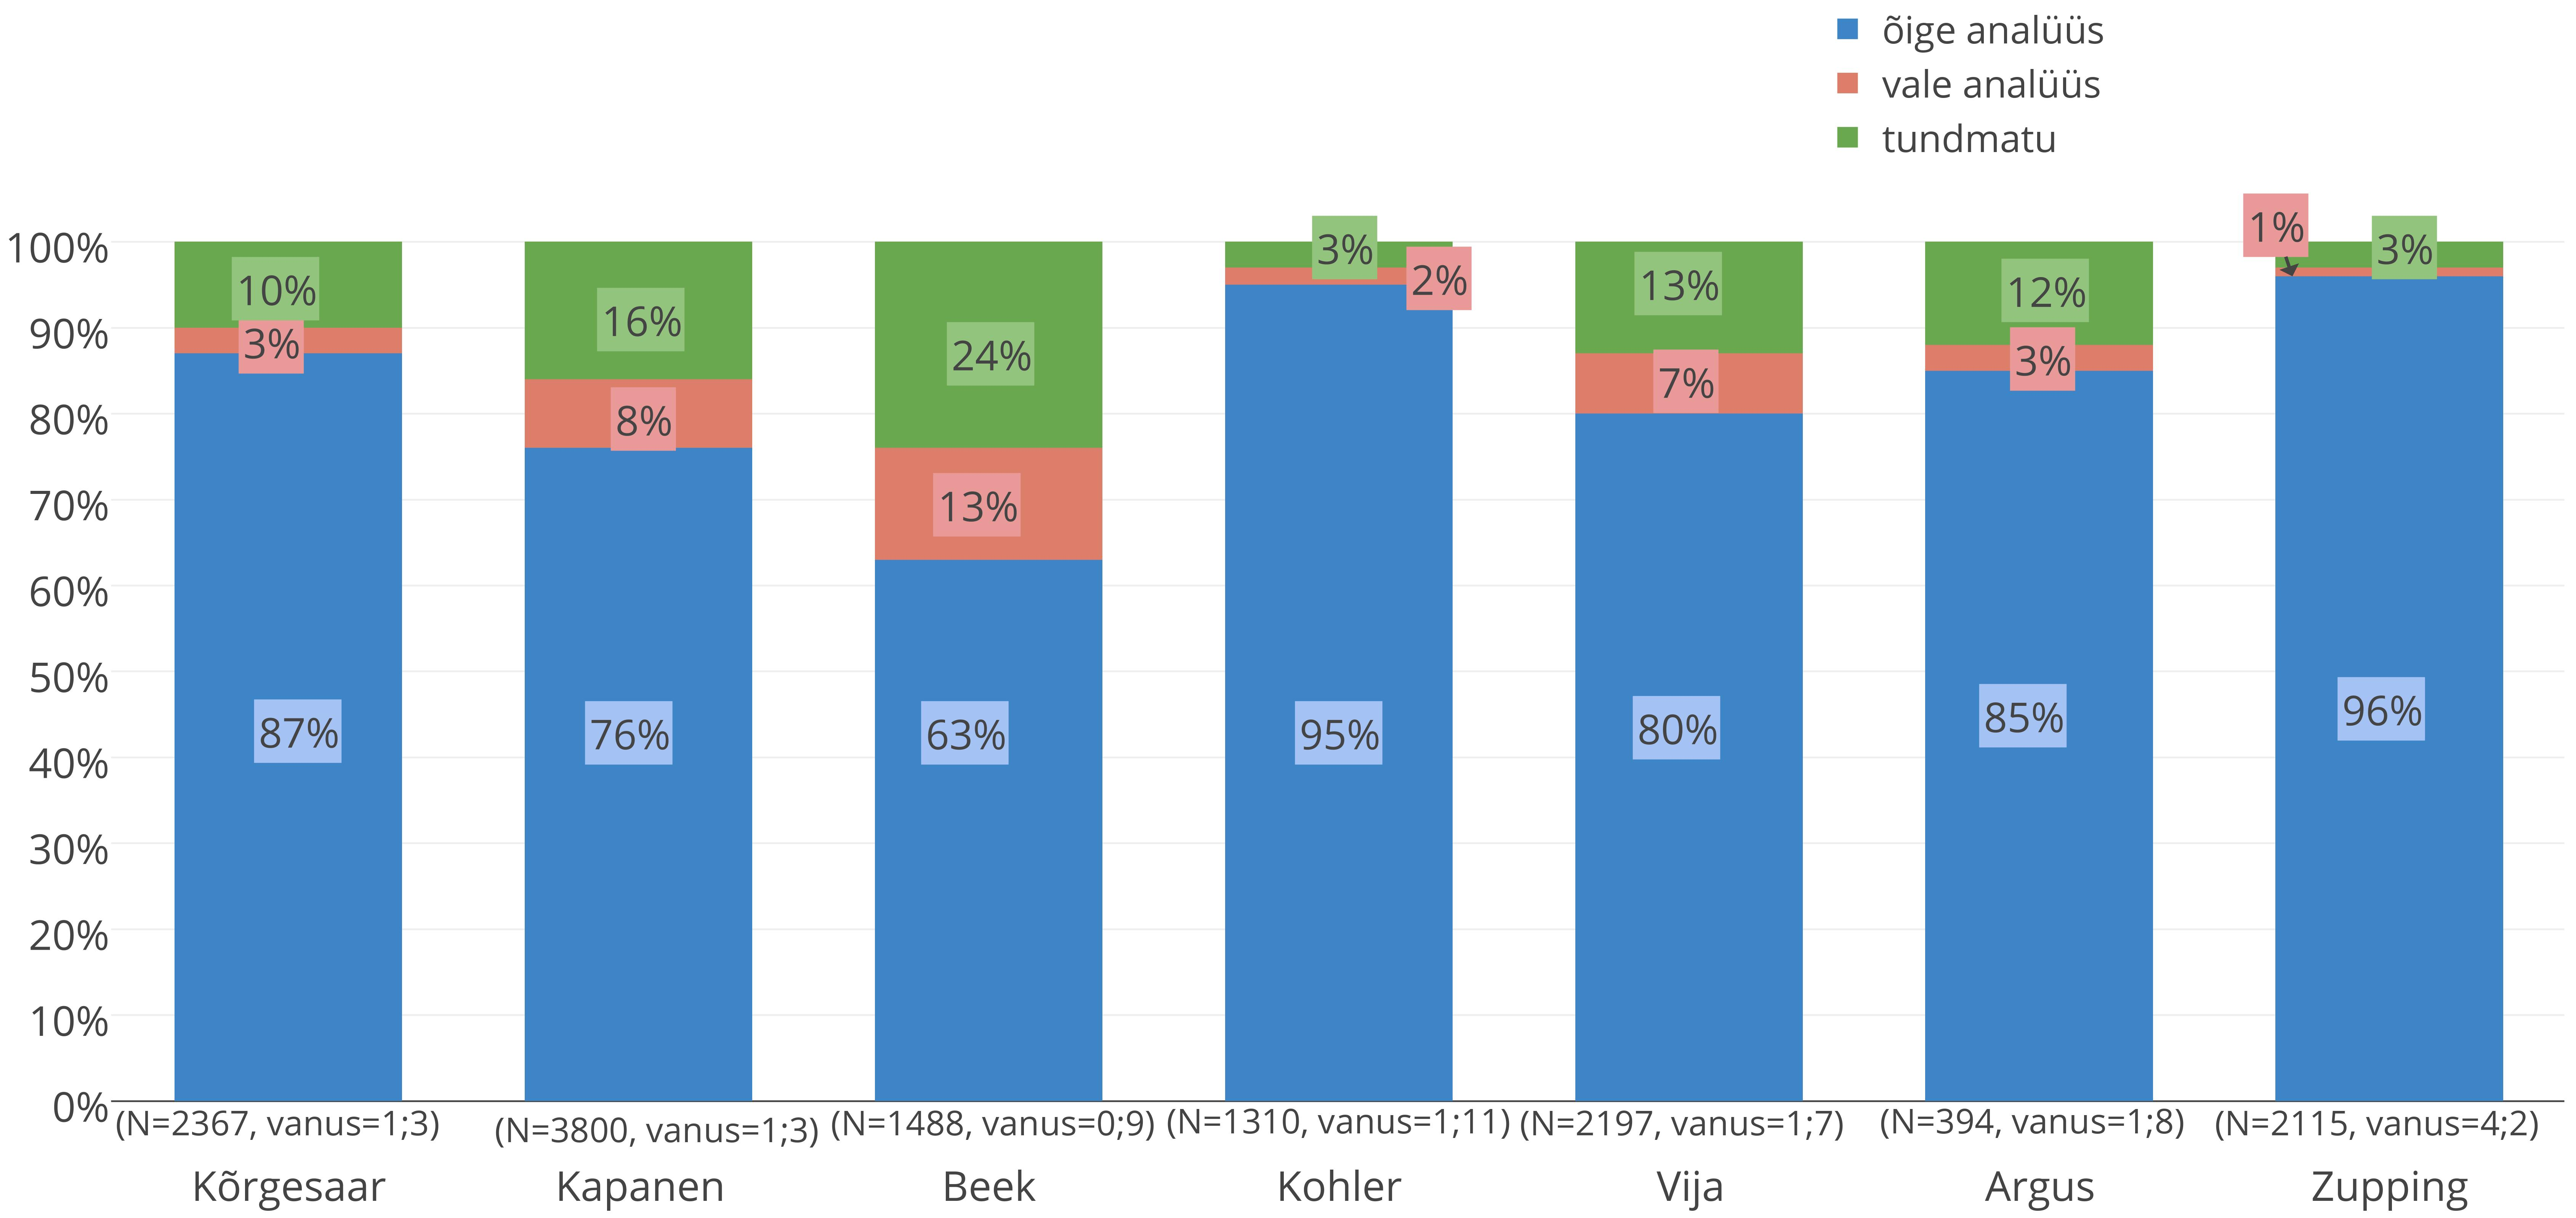
\includegraphics[width=\textwidth]{kasitsi_crop}
    \caption{tundmatud, õige ja vale analüüsi saanud sõnad alamkorpuse kaupa}
\end{figure}

Kõige paremad tulemused olid Zuppingu alamkorpuses, kus keelematerjal pärineb lindistusest lapsega vanuses 4;2. Kõikidest sõnadest oli vale analüüsi saanud sõnu vaid 1\%, õige analüüsi saanud sõnu 96\% ja tundmatuid sõnu 3\%. Kohleri alamkorpuses (lapse vanus 1;11) olid kõikidest sõnadest vale analüüsi saanud 2\%, õige analüüsi 95\% ja tundmatuks jäänud sõnu 3\%. Nii Arguse kui ka Kõrgesaare korpuses olid kõikidest sõnadest 3\% saanud vale analüüsi (Argusel laps vanuses 1;8 ja Kõrgesaarel 1;3). Vija alamkorpuses (laps vanuses 1;7) oli kõikidest sõnadest vale analüüsi saanud 7\%. Kapaneni korpuses (laps vanuses 1;3) oli 8\% sõnadest saanud vale analüüsi. Protsentuaalselt oli kõige enam vale analüüsi saanud sõnu (13\%) Beeki korpuses (laps vanuses 0;9).

Siinkohal tuleks muidugi tähelepanu pöörata ka sellele, et tekkinud on tahtmatu vanuseline järjestus -- kõige vähem vale analüüsi saanud sõnu on Zuppingu korpuses, kus lapse vanus on 4;2, ja kõige enam Beeki korpuses, kus lapse vanus on 0;9. Paraku pole vale analüüsi saanud sõnadel vanusega midagi pistmist, pigem on küsimus transkriptsioonide üleskirjutajas. Kui me vaatame Kapaneni ja Beeki alamkorpustes (vt tabel 4 ja 5) tundmatute ja vale analüüsi saanud sõnade osakaalu, siis näeme, et just neis korpustes on need kõige suuremad ja just nendes korpustes kasutatakse kõige enam nii lapse kui hoidja kõne transkribeerimisel kuuldeortograafiat ja sedagi mitte järjepidevalt. Näiteks Kapaneni ja Beeki korpuses kasutatakse läbisegi \emph{head isu} ja \emph{ead isu}, \emph{präegu} ja \emph{praegu}, \emph{jaaah} ja \emph{jah}, \emph{eiä} ja \emph{ei}, \emph{äitäh} ja \emph{aitäh} jne. Lisaks veel sõnaalgulised klusiilid \emph{buutuda} ja \emph{puutuda}, \emph{boti} ja \emph{poti}, \emph{balju} ja \emph{palju} jne. Selline üleskirjutusviis mõjutab ka morfoloogilise analüsaatori väljundit nii tundmatute kui ka vale analüüsi saanud sõnade osas, nt sõna \emph{ead} saab analüüsiks \emph{iga+d \_S\_ Pl Nom iga+d}, sõna \emph{präägust} saab analüüsiks \emph{prääk+0 \_S\_ Sg Gen}.


Täielikult vigadeta morfoloogiliselt märgendatud korpus eeldab, et iga sõnavorm saab õige sõnaliigilise kuuluvuse, käändsõnade puhul õige arvu ja käände, verbide puhul õige arvu, isiku, tegumoe, aja, kõneviisi ja kõnelaadi. Õige analüüsi valimine läheb keeruliseks siis, kui sõna paikneb kahe sõnaliigi vahel või kasutatakse teise sõnaliigi funktsioonis. Suur osa kategooriatest on vormi põhjal üheselt määratavad, kuid on selliseid mitteühesuse tüüpe, mis valmistavad isegi käsitsi määramisel raskusi, nt käändsõnad ja verbid, mille vormidest arenevad adpositsioonid ja adverbid (nt \emph{kätte}, \emph{käes}, \emph{alates}), verbi ja adjektiivi piirimail paiknevad partitsiibid (nt \emph{surnud}, \emph{kadunud}) ning adverbi ja konjunktsioonide piirimail paiknevad sõnad (nt \emph{aga}, \emph{nagu}, \emph{kui}). Morfoloogilise analüüsi mõttes oleks hea, kui sellist piirimail asetsemist oleks võimalikult vähe ja seetõttu peaksid sõnaliigid olema kirjeldatud nii, et ka süntaksit saaks võimalikult otstarbekalt kirjeldada. (\citealp[102--104]{Sonaliik}; \citealp[627--631]{Sonaliik2}).

Uue meedia korpuses võeti morfoloogilisel märgendamisel kasutusele partikli sõnaliik. Partikkel on muutumatu mittetäistähenduslik sõna, millel on eelkõige suhtluslik ja emotsionaalne funktsioon. \citep[4]{UUSMEEDIA} Ka lapsekeele korpuse puhul tuleks mõelda mõne uue sõnaliigi kasutusele võtmise peale. Näiteks, mida teha onomatopoeetiliste sõnadega? Onomatopoeetiliste sõnade rolli on alatähtsustatud, kuid olenemata sellest, kas keel on häälikusümboolika poolest rikas või mitte, kuuluvad onomatopoeetilised sõnad lapse esimeste sõnade hulka ja on ka hoidjakeeles sagedased (\citealp{Laing_1}; vt ka \citealp{Laing_2}). Reili Argus eristab onomatopoeetiliste sõnade hulgas ka \emph{imitatiive}, mis on onomatopoeetilised sõnad, mille häälikuline kuju võib olla varieeruv, kuid ei muutu morfoloogiliselt. Tüüpiliseks imitatiiviks on nt kiirabiauto signaali imiteeriv \emph{viuviu}, kõndmise väljendamiseks kasutatav \emph{tipa-tapa}. \citep[19--22]{IMITATIIV}

Lisaks sellele, et onomatopoeetiliste sõnade ja imitatiivide piir on hägune, on onomatopoeetilised sõnad ja imitatiivid ka lapse varases keelekasutuses sõnaliigililt mitmesed. \citep[20--21]{IMITATIIV} Eesti keele käsiraamat (\citealp{EKK}) jagab tähenduse järgi onomatopoeetilised sõnad interjektsioonide alla. Hennoste nimetab jällegi interjektsiooni sõnaliigiliseks prügikastiks, sest sinna on pandud kokku erinevad üksused. Hennoste arvates on onomatopoeetilised sõnad interjektioonide alla paigutatud sellepärast, et neil on kaldeline foneetiline ja fonoloogiline struktuur ning nad paiknevad sõna ja mittesõna piirimail. \citep[67]{Hennoste} Näites (1) ja (2) jääb imitatiivi sõnaliigiline kuuluvus segaseks:

(1)
\begin{description}
    \item *CHI: \textbf{addrr}, \textbf{drrr}, \textbf{brrr}
    \item *MOT: just, niimoodi sa õues sõidad vankriga \citep[27]{IMITATIIV}
\end{description}

(2)

\%comment: osutab autole paberil
\begin{description}
    \item *MOT: nii, tuled teen
    \item *MOT: sina tee katusele
    \item *CHI: \textbf{iiuiiu}
\end{description}
\%comment: Hendrik joonistab vilkureid \citep[28]{IMITATIIV}

Argus analüüsib neid nimisõnaks või verbiks \citep[28]{IMITATIIV}, kuid neid võib analüüsida isoleeritud onomatopoeetilisteks sõnadeks. Väidetakse, et enne presüntaktilist perioodi ongi raske sõnu liigitada ja sõnaliikidest saab alles siis rääkida, kui laps hakkab kasutama mitmesõnalisi väljendeid. Liigitusprobleemid tekivad eelkõige siis, kui sõnal puuduvad morfoloogilised ja süntaktilised tunnused. Kui lapse lausung on ilma morfoloogiliste tunnusteta, siis pole ka laiemast kontekstist kasu. \citep[27--29]{IMITATIIV}

Transkriptsioonide käsitsi läbivaatamise puhul hindasin seda, kas tegu on õige lemma, sõnaliigi ja morfoloogiliste kategooriatega. Vale analüüsi saanud sõnade puhul oli väga raske nende sõnaliigilist kuuluvust määrata, sest tihipeale polnud isegi konteksti olemasolul aru saada, millega tegu. Kui see valmistab juba inimesele probleeme, siis pole kahtluski, et analüsaator sellega hakkama saaks, sest tegu on kirjakeelest hälbiva tekstitüübiga. Vale analüüsi saanud sõnadest tegin sagedusloendi ja jaotasin need sõnad 5 erinevasse rühma.

\textbf{Esimese rühma} moodustavad onomatopeetilised sõnad: \emph{viu}, \emph{viuviu}, \emph{nämm}, \emph{amps}, \emph{mämmmämm}, \emph{mämm}, \emph{tapa}, \emph{summ}, \emph{pimm}, \emph{klõps}, \emph{pomm}, \emph{kiiga}, \emph{plaksu-plaksu}, \emph{patsu}, \emph{piiks-piiks-piiks-piiks}, \emph{piiks-piiks}, \emph{pats-pats-pats-pats}, \emph{amps}, \emph{kaak}, \emph{keps}, \emph{sulla}, \emph{kop}, \emph{mõmm}, \emph{põmm}, \emph{kaaga}, \emph{kõps}, \emph{patsu-patsu}, \emph{nämm}, \emph{pisspiss}, \emph{köhi}, \emph{aia}, \emph{tiks}. Nendele sõnadele oli raske sõnaliigilist kuuluvust määrata, mistõttu paigutasin ``kirvemeetodil'' kõik helijäljenduslikud sõnad ühte rühma.


\textbf{Teise rühma} moodustavad häälitsused ja sõnad, mille tähendusest pole võimalik aru saada ka konteksti olemasolul: \emph{paa}, \emph{eo}, \emph{änn}, \emph{t}, \emph{pupe}, \emph{pigi}, \emph{op}, \emph{muks}, \emph{kookai}, \emph{kaka}, \emph{jää}, \emph{manni}, \emph{öö}, \emph{ämm}, \emph{mm}, \emph{a}, \emph{ä}, \emph{s}, \emph{emm}, \emph{mm}.

\textbf{Kolmanda rühma} moodustavad pärisnimed, mis puuduvad morfoloogilise analüsaatori leksikonist: \emph{Tiibu}, \emph{Triibu}, \emph{Liisu}, \emph{Tups}, \emph{Tuksi}, \emph{Carlos}, \emph{Sirts}, \emph{Sirtsu}, \emph{Annika}, \emph{Antsu}, \emph{Pitsu}, \emph{Alari}.

\textbf{Neljanda rühma} moodustavad sõnad, mis saavad, kas vale lemma või sõnaliigi: 
\emph{mõmmi}, \emph{siuke}, \emph{venna}, \emph{tudu}, \emph{pai}, \emph{siukse}, \emph{nuku}, \emph{kalli-kalli}, \emph{kalli}, \emph{vot-vot}, \emph{tantsi-tantsi}, \emph{näri-näri}, \emph{mida-mida}, \emph{musi-musi}, \emph{kapp-kapp}, \emph{kapp-kapp-kapp-kapp}, \emph{istu-istu}, \emph{aitab-aitab}, \emph{aluspüksid-aluspüksid-aluspüksid}, \emph{ruttu-ruttu-ruttu}, \emph{väga-väga}, \emph{ja-ja-ja}, \emph{et-et-et}, \emph{tule-tule}, \emph{pisspissi}, \emph{mine-mine}. Siia alla kuuluvad ka sõnad nagu \emph{kuule}, \emph{palun}, \emph{näe}. Need sõnad on siin seetõttu, et need paiknevad verbi ja interjektsiooni piirimail ning oleksid justkui tekkinud täistähenduslike sõnade muutumise teel.

\textbf{Viienda rühma} moodustavad sõnad, mis on oma vormilt vigased (st on läbinud teatud täheteisendused) ja mida CHILDES-i transkriptsioonisüsteemis kodeeritakse [\emph{= explanation}] abil: \emph{ütted} (\emph{ütled}), \emph{ükskold} (\emph{ükskord}), \emph{pilukat} (\emph{pirukas}), \emph{ea} (\emph{hea}), \emph{kah} (\emph{diktofon}), \emph{tee} (\emph{terve}), \emph{kesse} (\emph{kes see}), \emph{emmmee} (\emph{emme}), \emph{auh} (\emph{arvuti}), \emph{te} (\emph{see}), \emph{papa} (\emph{kõndima}), \emph{lau} (\emph{laud}), \emph{kiku} (\emph{diktofon}), \emph{kolla} (\emph{kollane}), \emph{teda} (\emph{seda}), \emph{täh} (\emph{aitäh}), \emph{laua} (\emph{laulma}), \emph{kuku} (\emph{luku}), \emph{kiigu} (\emph{kiik}), \emph{au} (\emph{arvuti}), \emph{olla} (\emph{alla}), \emph{määgu} (\emph{mänguasjad}), \emph{kukk} (\emph{trukk} või \emph{raamat}), \emph{koss} (\emph{koos}), \emph{kõrre} (\emph{kõrgel}), \emph{katte} (\emph{kätte}), \emph{kurki} (\emph{kurku}), \emph{noosi} (\emph{joonista}), \emph{kispi} (\emph{küpsis}), \emph{takku} (\emph{traktor}), \emph{ots} (\emph{otsas}), \emph{mammu} (\emph{mari}), \emph{äi} (\emph{ai}), \emph{utu} (\emph{lutt}), \emph{kiika} (\emph{kiikuda}), \emph{kass} (\emph{kastis}), \emph{kapi} (\emph{käbi}), \emph{takka} (\emph{traktor}), \emph{ussi} (\emph{sussid}), \emph{eita} (\emph{ei taha}), \emph{ängi} (\emph{mängib}), \emph{väigi} (\emph{värvi}), \emph{uu} (\emph{õun}), \emph{uksi} (\emph{nutikas}), \emph{toodi} (\emph{joonista}), \emph{tisse} (\emph{televiisori}), \emph{tahta} (\emph{tahan}), \emph{sea} (\emph{see}), \emph{raama} (\emph{raamat}), \emph{puusi} (\emph{pluusi}), \emph{puuniks} (\emph{pruuniks}), \emph{pusti} (\emph{püsti}), \emph{punnu} (\emph{punnis}), \emph{präägust}, \emph{pettu} (\emph{peitu}), \emph{palu} (\emph{palun}), \emph{memme} (\emph{me me}), \emph{märgi} (\emph{värvi}), \emph{mängu} (\emph{mänguasjad}), \emph{mähku} (\emph{mähe}), \emph{laadi} (\emph{lahti}), \emph{kuudi} (\emph{uurima}), \emph{kumme} (\emph{kolm}), \emph{ku} (\emph{diktofon}), \emph{koo} (\emph{koos}), \emph{kõne} (\emph{põnev}), \emph{kombe} (\emph{kombekas}), \emph{kiidu} (\emph{kiisu}), \emph{kii} (\emph{diktofon}), \emph{kat} (\emph{kaks}), \emph{kalju} (\emph{karu}), \emph{kaapi} (\emph{kapi}), \emph{boodi} (\emph{voodi}), \emph{aula} (\emph{laulda}), \emph{auk} (\emph{arvuti}), \emph{aru} (\emph{arvuti}), \emph{ala} (\emph{sajajalgne}), \emph{kipsist} (\emph{küpsist}), \emph{kiisupilt} (\emph{kiisu pilt}), \emph{keti} (\emph{kõdi}), \emph{lutu} (\emph{lutt}), \emph{kumme} (\emph{kummikud}), \emph{sala} (\emph{sajajalgne}), \emph{pillu} (\emph{piilub}), \emph{patt} (\emph{part}), \emph{panni} (\emph{banaanid}), \emph{paa} (\emph{maal}), \emph{olu} (\emph{orav}), \emph{oa} (\emph{orav}), \emph{süü} (\emph{süüa}), \emph{sunni} (\emph{sünnipäev}), \emph{punni} (\emph{punnis}), \emph{käia} (\emph{käima}), \emph{võta} (\emph{võtta}), \emph{õue} (\emph{õues}), \emph{maitse} (\emph{maitsevad}), \emph{koti} (\emph{kott}), \emph{mai} (\emph{mari}), \emph{aua} (\emph{koer}), \emph{voot} (\emph{vot}), \emph{Kate} (\emph{Kattre}).

Tundmatute ning vale analüüsi saanud sõnade hulka saab vähendada analüsaatori allkeelespetsiifilisemaks muutmise teel. Analüsaatori käitumise kohandamiseks tuleks anda sellele sobiv kasutajasõnastik. Kasutajasõnastik on fail, kus igal real on analüüsitav sõnavorm ja selle analüüs. Iga sõna korral kontrollib analüsaator esmalt, kas sõna on kasutajasõnastikus või mitte. Kui on, siis võetakse sealt sõna analüüs, kui ei, siis minnakse morfoloogilist analüüsi tegema. Nii saab kasutajasõnastikku panna sõnu, mida analüsaator muidu analüüsida ei suudaks, ja sõnu, mis peaksid konkreetses tekstis teistsuguse analüüsi saama.

Esimesese rühma ehk onomatopoeetiliste sõnade puhul on raske nende sõnaliigilist kuuluvust määrata, seega tuleks mõelda kasutajasõnastikus uue sõnaliigi defineerimise peale. Teine küsimus on selles, kuidas onomatopoeetilisi sõnu tuvastada? CHILDES-i transkriptsioonisüsteemis on omajagu spetsiifilisi märgendusi, mida on võimalik igale sõnale külge liita. Onomatopoeetiliste sõnade markeerimiseks esitatakse märgendus \underline{@o} --> \emph{piip}@o, \emph{summ}@o \emph{summ}@o. Sellist tüüpi märgenduse kasutamine teeks onomatopoeetilised sõnad nähtavaks ja oluliselt lihtsustaks nende ekstraheerimist. Kui need sõnad on tuvastatavad, siis on võimalik neid ka automaatselt kasutajasõnastikku lisada. Ainsana on onomatopoeetiliste sõnade markeerimist kasutatud Vija alamkorpuses (781 korral). Seega, praegune olukord näeb ette seda, et onomatopoeetiliste sõnade tuvastamiseks tuleb palju käsitööd teha.

Teise rühma kuuluvad häälitsused ja sõnad, mille tähendusest pole isegi konteksti olemasolul võimalik aru saada. Loomulikult ei tasu juuksekarva lõhki ajada, kuid sellised sõnad on analüsaatori jaoks problemaatilised. Näiteks \emph{t}, \emph{op},  \emph{mm}, \emph{a}, \emph{ä}, \emph{s}, \emph{emm}, \emph{mm} analüüsitakse lühenditeks. Selliste ühe või mitmetäheliste ``sõnade'' valesti analüüsimise vältimiseks ja tuvastamiseks piisaks, kui kasutada spetsiifilist märgendust @\emph{k} (mitme tähe jaoks) või @\emph{l} (ühe tähe jaoks). @\emph{l} märgendust on kasutatud Vija (343x), Zuppingu (3x) ja Kohleri (41x) alamkorpustes. ``Sõna'' \emph{eo} saab analüüsiks \emph{idu+0 \_S\_ Sg Gen}, kuid konteksti vaadates saab aru, et laps ei räägi idudest, vaid tegemist on silbitamisega. Ja selliste sõnade nagu \emph{kaka}, \emph{öö}, \emph{ämm} puhul on tegemist häälitsustega, kuid analüsaatori jaoks näevad need välja kui traditsioonilised eesti keele sõnad ja seetõttu saavad vale analüüsi.

Kolmanda ja neljanda rühma sõnade valesti analüüsimise vastu ei saa üleskirjutaja midagi teha. Kolmanda rühma sõnad ehk pärisnimed puuduvad analüsaatori kasutajasõnastikust, aga et nende kirjapilt sarnaneb teistele eestikeelsetele sõnadele, siis saavad need ka vale analüüsi. Neljandas rühmas on palju reduplikatiivseid sõnu, mille puhul on analüsaator õigesti analüüsinud nende sõnaliigi ja morfoloogilised kategooriad, kuid on andnud vale lemma, nt \emph{väga-väga+0 \_D\_}, \emph{mine-mine+0 \_V\_ Pers Prs Imprt Sg2}. Lisaks on seal sellised sõnad, mis on muidu astmevahelduslikud, kuid on nihutatud astmevahelduseta tüüpi, nagu 
\emph{mõmmi}, \emph{venna}, \emph{nuku}, mida analüüsitakse genitiivivormideks. Kolmanda ja neljanda rühma sõnade tuvastamiseks ja kasutajasõnastiku täiendamiseks tuleb transkriptsioone palju käsitsi üle vaadata.

Viienda rühma sõnad moodustavad sõnad, mis on oma vormilt vigased (st läbinud teatud täheteisendused) ja mida CHILDES-i transkriptsioonisüsteemis kodeeritakse [\emph{= explanation}] abil. Alapeatükis 3.2 kirjutasin mõningatest standardiseerimise probleemidest, mis puudutavad ka viienda rühma sõnu. Nimelt, asi saab alguse juba sellest, et üleskirjutaja peab keelematerjali transkribeerimisel tegema kaht tüüpi otsuseid, mida tuleb usaldusväärsuse saavutamiseks pidevalt järgida. Esmalt peab üleskirjutaja otsustama, kas konkreetne keeleline üksus vastab normile või mitte. See otsus sõltub otseselt üleskirjutaja intuitsioonist. Teine otsus puudutab vea määratlemist ja selle kodeerimist. CHILDES-i transkriptsioonisüsteemis on vigade kodeerimiseks mitmeid võimalusi (vt ptk 3.2 näide (2) ja (3)). Lisaks [*] ja [: \emph{tegelik\_sõna}] kodeeringutele, kasutatakse ka n-ö tõlke kodeeringut [= \emph{explanation}], nt \emph{tööt} [= \emph{tööd}] (Kapanen, 01.cha). Nimetame loetavuse mõttes [: ] kodeeringut I tüüpi, [= ] kodeeringut II tüüpi ja [*] III tüüpi vealiigiks. Tabel 10 annab ülevaate sellest, mis tüüpi ja kui palju on veakodeeringuid alamkorpustes kasutatud.

\begin{table}[H]
\centering
\caption{vealiigitamine alamkorpustes}
\begin{tabular}{|l|c|c|c|}
\hline
korpus    & I tüüp: {[}: tegelik\_sõna{]} & II tüüp: {[}= tõlge{]} & III tüüp: {[}*{]} \\ \hline\hline
Argus     & 522                   & -             & -       \\ \hline
Beek      & 43                    & -             & -       \\ \hline
Kapanen   & 9                     & 1198          & -       \\ \hline
Kõrgesaar & 280                   & 1219          & -       \\ \hline
Kohler    & 2062                  & 173           & -       \\ \hline
Vija      & 8534                  & 3122          & 547     \\ \hline
Zupping   & -                     & 2883          & -       \\ \hline
\end{tabular}
\end{table}

Vealiigitamisest on oluline rääkida sellepärast, et see mõjutab otseselt morfoloogilise analüsaatori tööd. Morfoloogilise info lisamine puudutab just I tüüpi vealiiki (vt ptk 4.1 ja 4.1.2), sest need teisendatakse XML-is \emph{<replacement>}-elementideks. Morfoloogilise info lisamise käigus analüüsib programm just neid elemente, kuid mitte II tüübi sees olevat sõna või III tüübile eelnevat sõna. Ka CLAN-programm järgib sama põhimõtet. Viienda rühma sõnade puhul on kasutatud II tüüpi liigitamist, mistõttu saavad need ka vale analüüsi. Paraku pole võimalik analüüsida II tüüpi vealiigi sees olevaid sõnu, kuna nende asukoht pole kindlalt fikseeritud. Näiteks [: ] kodeering peab vigasele vormile vahetult järgnema (\emph{pitti} [: \emph{pilti}], Vija 10724.cha), kuid [= ] võib järgneda nii üksikule sõnale kui ka tervele lausungile (nt \emph{mõh} [= \emph{mõmmi}] \emph{kodu} vs \emph{õmmi teep} [= \emph{mõmmi teeb}], Kapanen 01.cha).

Kui vaadata alamkorpustes tundmatuks jäänud sõnu (vt tabelid 3--9) ja üleskirjutaja vealiigitamist (vt tabel 10), siis võib märgata teatud seost. Korpustes, kus kasutatakse I tüüpi liigitamist, on ka üldjuhul vähem tundmatuks jäänud sõnu, nt Vija, Kohleri ja Kõrgesaare alamkorpus. Beeki korpuses kasutatakse ainult I tüüpi liigitamist, kuid sedagi iseäranis vähe, ning lapse tundmatuks jäänud ja vale analüüsi saanud sõnade hulk on korpuses suur. See viitab jällegi sellele, et lapse keelekasutuse üleskirjutamisel kasutatakse palju kuuldeortograafiat ning hoidjakeelt kirjutatakse üles kirjakeelele sarnaselt. Kapaneni korpuses kasutatakse rohkelt II tüüpi liigitamist, kuid esmase analüüsi tulemustele need palju kaasa ei aita. Ka Kapaneni korpuses kasutatakse lapsekeele üleskirjutamisel palju kuuldeortograafiat ja hoidjakeele puhul lähtutakse kirjakeele normist. Zuppingu korpuse ei esine I tüüpi vealiigitamist ning lapse tundmatuks jäänud sõnade osakaal on suur (vt tabel 9), mis viitab samuti sellele, et lapse keelekasutust märgitakse üles häälduspäraselt ja hoidjakeelt kirjakeelele sarnaselt.

Selle alapeatüki eesmärk pole anda korpuste transkribeerimisele hinnangut, vaid esitada objektiivseid tähelepanekuid ja soovitusi, mis võiksid morfoloogilise analüüsaatori väljundit paremaks muuta. Hennoste kirjutab, et suulise kõne transkriptsiooni koostamisel on kaks printsiipi. Esimene printsiip on autentsus ehk transkriptsioonis peab säilima informatsioon, mis on suhtluse loomuse suhtes tõene. Teine printsiip on praktilisus ehk transkribeerimise tavad peavad olema andmete korraldamise ja analüüsi viisi suhtes praktilised. See tähendab seda, et märgendada tuleb neid nähtuseid, mida uurijal on tarvis, kuid et see üldist pilti üle ei küllastaks. \citep[92--93]{Hennoste} Küsimus ei ole selles, et korpuse tegija peab kvaliteetsema analüüsi nimel loobuma autentsusest ja praktilisusest, vaid selles, kas transkribeerija on nõus natuke rohkem vaeva nägema ja valmis üles märkima nii vigaseid (ehk mida laps tegelikult ütles) kui õigeid (ehk öeldu kirjakeelne variant) vorme. On arusaadav, et iga transkriptsioon on üles kirjutatud vastavalt uurija eesmärkidele, kuid siinkohal tuleks mõelda sellele, kuidas selline üleskirjutamise viis mõjutab sellele järgnevat analüüsi ja töötlust.

\newpage
\section{Edasine töö}

Selles töös jõuti lapsekeele korpuse morfoloogilise analüüsimise esimese katsetuseni. Selles osas annangi ülevaate sellest, kuidas korpusega edasi toimida ehk kuidas oleks võimalik korpuse morfoloogilise analüüsi kvaliteeti tõsta.

\textbf{Kasutajasõnastik}: selleks, et tundmatute ning vale analüüsi saanud sõnade hulka vähendada, tuleks morfoloogilise analüsaatori käitumist muuta. Kasutajasõnastiku tegemiseks oleks tarvis tundmatuid sõnu lähemalt vaadata. Järgnevalt esitan iga alamkorpuse 20 kõige sagedasemat tundmatut sõnavormi (sulgudes olev arv tähistab selle esinemissagedust alamkorpuses).

\textbf{Kõrgesaar}: \emph{vä} (651), \emph{nimodi} (251), \emph{ää} (234), \emph{brmm} (166), \emph{ästi} (129), \emph{nooh} (109), \emph{onju} (104), \emph{präegu} (100), \emph{allo} (97), \emph{Sirlin} (96), \emph{tegelt} (93), \emph{aah} (89), \emph{eksole} (80), \emph{mmh} (69), \emph{mmm} (64), \emph{Demi} (60), \emph{niimodi} (54), \emph{süia} (51), \emph{brumm} (48), \emph{ops} (47).

\textbf{Vija}: \emph{vä} (459), \emph{kessee} (219), \emph{Atsu} (107), \emph{ähäh} (92), \emph{tip} (75), \emph{part\_Toomas} (69), \emph{nooh} (68), \emph{mkmm} (66), \emph{sis} (62), \emph{ää} (54), \emph{ahsoo} (45), \emph{taa} (36), \emph{eksju} (36), \emph{niimodi} (36), \emph{jahh} (35), \emph{tsuhh} (33), \emph{trikstraks} (33), \emph{vat} (32), \emph{mmm} (32), \emph{pss} (30).

\textbf{Beek}: \emph{äta} (758), \emph{vä} (727), \emph{mmh} (339), \emph{mmm} (325), \emph{enna} (287), \emph{Liisbet} (282), \emph{onju} (172), \emph{hõõ} (166), \emph{ääh} (158), \emph{äää} (153), \emph{ää} (120), \emph{aah} (120), \emph{äääh} (110), \emph{ops} (104), \emph{eiä} (86), \emph{õõh} (69), \emph{aaah} (68), \emph{õõ} (65), \emph{mmmm} (65), \emph{ääää} (62).

\textbf{Kapanen}: \emph{Lote} (209), \emph{Martiina} (168), \emph{kaa} (160), \emph{vä} (70), \emph{ää} (68), \emph{mmm} (65), \emph{sis} (46), \emph{äla} (44), \emph{tan} (43), \emph{präegu} (42), \emph{nimodi} (36), \emph{aah} (33), \emph{süia} (33), \emph{puttu} (32), \emph{vata} (31), \emph{ästi} (24), \emph{taa} (24), \emph{ku} (24), \emph{tipa} (21), \emph{näedsa} (20).

\textbf{Argus}: \emph{kaa} (159), \emph{Ninnu} (117), \emph{enna} (41), \emph{drra} (37), \emph{ätaäta} (35), \emph{tiia} (27), \emph{iu} (20), \emph{mäu} (19), \emph{rra} (19), \emph{mämmib} (16), \emph{tiit} (16), \emph{akka} (16), \emph{iiu} (15), \emph{telle} (14), \emph{põrra} (14), \emph{pisi} (13), \emph{atata} (13), \emph{nooh} (13), \emph{iuiu} (12), \emph{plla} (12).

\textbf{Kohler}: \emph{Taimo} (162), \emph{Stella} (143), \emph{Vallu} (71), \emph{Sandor} (70), \emph{allo} (55), \emph{kiss} (54), \emph{aiai} (44), \emph{tak} (39), \emph{onju} (38), \emph{hoppa} (37), \emph{garaazhi} (34), \emph{opa} (31), \emph{Sanna} (29), \emph{miau} (25), \emph{tsuh} (24), \emph{mõmmit} (24), \emph{tit} (22), \emph{tapa} (19), \emph{Kelly} (18), \emph{Sandori} (16).

\textbf{Zupping}: \emph{onju} (83), \emph{äla} (76), \emph{ää} (48), \emph{Eddy} (32), \emph{mõnna} (31), \emph{vä} (29), \emph{mmm} (28), \emph{taan} (27), \emph{jee} (26), \emph{opa} (26), \emph{enna} (25), \emph{daa} (25), \emph{opsti} (24), \emph{pika} (24), \emph{älle} (23), \emph{Ipa} (23), \emph{Krissu} (21), \emph{oih} (20), \emph{numbe} (20), \emph{koppadi} (19).

Iga alamkorpuse sõnavorme vaadates märkame sarnaseid sõnaliike:

\begin{itemize}
    \item pärisnimed: \emph{Sirlin}, \emph{Atsu}, \emph{Liisbet}, \emph{Lote}, \emph{Martiina}, \emph{Ninnu}, \emph{Taimo}, \emph{Stella}, \emph{Vallu}, \emph{Sandor}, \emph{Sanna}, \emph{Kelly}, \emph{Demi}, \emph{Sandori}, \emph{Eddy}, \emph{Ipa}, \emph{Krissu};
    \item häälitsused: \emph{ää}, \emph{mmm}, \emph{ätaäta/atata} ja nende erinevad variatsioonid;
    \item partiklid: \emph{noh}, \emph{aah}, \emph{jahh} ja nende erinevad variatsioonid;
    \item sõna lühendamine: \emph{vata}, \emph{tegelt}, \emph{vä};
    \item kokku liidetud sõnad: \emph{onju}, \emph{eksole}, \emph{ahsoo}, \emph{eksju}, \emph{näedsa};
    \item häälduspärane üleskirjutus: \emph{nimodi} ja selle variatsioonid, \emph{präegu}, \emph{enna} (\emph{venna}), \emph{sis} (\emph{siis}), \emph{älle} (\emph{jälle}), \emph{äla} (\emph{ära}), \emph{taan} (\emph{tahan}).
\end{itemize}

Traditsioonilisest sõnaliigi jaotumisest ei piisa (nt häälitsuste ja onomatopoeetiliste sõnade jaoks), kuid täpsema tegevusplaani jaoks peab tundmatuks jäänud ja ka vale analüüsi saanud sõnu põhjalikumalt analüüsima. Kasutajasõnastiku tegemise puhul tuleb arvestada ka korpuse ja selle sõnavaraga. On tehtud kindlaks, et sõna sagedused järgivad Zipfi seadust. Zipf leidis, et sagedusel ning selle astakul (sõna järjekorranumber sageduste kahanevas reas) sagedussõnastikus on suure dokumendi puhul sõltuvuses ehk siis sõna sagedusel ja selle astaku vahel on funktsionaalne seos, vt \citep[ptk 1]{Baayen}. Lihtsamalt lahti seletatuna tähendab see seda, et meil on leksikonis väike hulk sõnu, mis on väga sagedased, ja suur hulk sõnu, mida esineb väga harva. Eelnevalt tõin välja need kõige sagedasemad sõnavormid igas alamkorpuses, aga tabelis 10 on esitatud tundmatuks jäänud sõnavormide (ja neist vaid ühe korra esinevate sõnavormide) koguarv igas alamkorpuses. Tabelist on näha, et vaid ühe korra esinevaid sõnavorme igas korpuses on väga palju, varieerudes 51 ja 74\% vahel. Korpuse morfoloogilise analüüsi kvaliteedi parandamisel tuleks sellega ka kindlasti arvestada.

\begin{table}[H]
\centering
\caption{tundmatute ning 1x esinevate sõnavormide arv ja \%}
\begin{tabular}{|l|c|c|}
\hline
korpus    & \multicolumn{1}{l|}{tundmatuks jäänud sõnavormid} & \multicolumn{1}{l|}{1x tundmatuks jäänud vormid}      \\ \hline\hline
Vija      & 1901                                              & \begin{tabular}[c]{@{}c@{}}1197\\ 63\%\end{tabular} \\ \hline
Beek      & 1555                                              & \begin{tabular}[c]{@{}c@{}}1003\\ 65\%\end{tabular} \\ \hline
Kapanen   & 2469                                              & \begin{tabular}[c]{@{}c@{}}1828\\ 74\%\end{tabular} \\ \hline
Argus     & 221                                               & \begin{tabular}[c]{@{}c@{}}113\\ 51\%\end{tabular}  \\ \hline
Kohler    & 432                                               & \begin{tabular}[c]{@{}c@{}}245\\ 57\%\end{tabular}  \\ \hline
Kõrgesaar & 3551                                              & \begin{tabular}[c]{@{}c@{}}2372\\ 67\%\end{tabular} \\ \hline
Zupping   & 1355                                              & \begin{tabular}[c]{@{}c@{}}848\\ 63\%\end{tabular}  \\ \hline
\end{tabular}
\end{table}

\textbf{Korpuse märgendamise ja standardiseerimise paremaks muutmine}: spontaanse kõne lindistamine ja üleskirjutamine on kahtlemata väga töö- ja ajamahukas, kuid selle töö käigus on kerkinud üles mitmeid üleskirjutamise kitsaskohti (vt ka ptk 4.2).

Üheks kitsaskohaks on onomatopoeetilised sõnad ja häälitsused. CHILDES-i konventsioonide järgi on iga sõna külge võimalik liita spetsiaalseid märgendusi: \underline{@o} on onomatopoeetilise sõna markeerimiseks, \underline{@x} saab kasutada sõna välja jätmiseks, \underline{@k} abil saab silpe markeerida, \underline{@l} abil saab ühte häälikut markeerida, \underline{@c} ehk lapse väljamõeldud vormi markeerimiseks, \underline{@z} abil saab transkribeerija kasutada oma defineeritud märgendust jpm. Hetkeolukord näeb ette, et kasutajasõnastikku täiendatakse käsitsi, kuid spetsiaalsete märgenduste kasutamine võimaldaks seda automaatselt teha.

Teiseks suureks kitsaskohaks on sellised sõnad, mis on läbinud teatud täheteisendused. Osad transkribeerijad on lapse poolt öeldut kirjakeelsemaks muutnud, osad jällegi kasutavad üleskirjutamisel palju kuuldeortograafiat (ja sedagi ebajärjepidevalt). Morfoloogilise analüüsi seisukohalt on hetkeolukord selline, et suur osa vale analüüsi saanud (vt ptk 4.2 esitatud viiendat sõnarühma) ja tundmatuks jäänud sõnu sõltuvad paraku üleskirjutamise viisist. Korpuse tegija ei pea kvaliteetsema analüüsi nimel loobuma autentsusest ja praktilisusest. Küsimus on pigem selles, kas transkribeerija on nõus natuke rohkem vaeva nägema ja valmis kodeerima nii vigaseid (ehk mida laps tegelikult ütles) kui ka nende õigeid (ehk öeldu kirjakeelne variant) vorme.


\textbf{Korpuse ühestamine}: korpus on praegusel kujul ühestamata, see tähendab, et kõikvõimalikud analüüsid on alles jäetud. Pikemas perspektiivis on kindlasti plaan teha nii, et iga sõna saaks vaid ühe analüüsivariandi, kuid see nõuab palju käsitsi üle vaatamist.


\newpage
\addcontentsline{toc}{section}{Kokkuvõte}
\section*{Kokkuvõte}
TEEN TÄNA, OLENEB MUIDUGI ANALÜÜSI PEATÜKKIDEST.

\newpage
\addcontentsline{toc}{section}{Summary}
\section*{Summary}

\newpage
\addcontentsline{toc}{section}{Lisad}
\section*{Lisad}
\textbf{Lisa 1. Vija}

\begin{table}[H]
\centering
\resizebox{\textwidth}{!}{
\begin{tabular}{|l|l|c|c|c|c|c|}
\hline
Lapse nimi               & Vanus    & \multicolumn{1}{l|}{Sugu} & \multicolumn{1}{l|}{Sessioonid} & \multicolumn{1}{l|}{Lapse sõnad} & \multicolumn{1}{l|}{Hoidja sõnad} & \multicolumn{1}{l|}{KOKKU} \\ \hline\hline
\multirow{3}{*}{Andreas} & 1;7-1;11 & \multirow{3}{*}{p}        & 7                               & 2845                             & 8521                              & 11366                      \\ \cline{2-2} \cline{4-7} 
                         & 2;0-2;8  &                           & 37                              & 41498                            & 59272                             & 100770                     \\ \cline{2-2} \cline{4-7} 
                         & 3;0-3;1  &                           & 30                              & 66038                            & 48137                             & 114175                     \\ \hline\hline
KOKKU                    & \multicolumn{2}{l|}{}                & 74                              & 110381                           & 115930                            & 226311                     \\ \hline
\end{tabular}}
\end{table}
\hfill

\textbf{Lisa 2. Argus}

\begin{table}[H]
\centering
\resizebox{\textwidth}{!}{
\begin{tabular}{|l|l|c|c|c|c|c|}
\hline
Lapse nimi               & Vanus    & \multicolumn{1}{l|}{Sugu} & \multicolumn{1}{l|}{Sessioonid} & \multicolumn{1}{l|}{Lapse sõnad} & \multicolumn{1}{l|}{Hoidja sõnad} & \multicolumn{1}{l|}{KOKKU} \\ \hline\hline
\multirow{2}{*}{Hendrik} & 1;8-1;11 & \multirow{2}{*}{p}        & 5                               & 566                              & 1963                              & 2529                       \\ \cline{2-2} \cline{4-7} 
                         & 2;0-2;5  &                           & 12                              & 3654                             & 7190                              & 10844                      \\ \hline\hline
KOKKU                    & \multicolumn{2}{l|}{}                & 17                              & 4220                             & 9153                              & 13373                      \\ \hline
\end{tabular}}
\end{table}
\hfill

\textbf{Lisa 3. Beek}

\begin{table}[H]
\centering
\resizebox{\textwidth}{!}{
\begin{tabular}{|l|l|c|c|c|c|c|}
\hline
Lapse nimi               & Vanus    & \multicolumn{1}{l|}{Sugu} & \multicolumn{1}{l|}{Sessioonid} & \multicolumn{1}{l|}{Lapse sõnad} & \multicolumn{1}{l|}{Hoidja sõnad} & \multicolumn{1}{l|}{KOKKU} \\ \hline\hline
\multirow{3}{*}{Liisbet} & 0;9-0;11 & \multirow{3}{*}{t}        & 6                               & 1450                             & 11487                             & 12937                      \\ \cline{2-2} \cline{4-7} 
                         & 1;0-1;2  &                           & 5                               & 1143                             & 10463                             & 11606                      \\ \cline{2-2} \cline{4-7} 
                         & 2;0-2;5  &                           & 9                               & 7571                             & 27022                             & 34593                      \\ \hline\hline
KOKKU                    & \multicolumn{2}{l|}{}                & 20                              & 10164                            & 48972                             & 59136                      \\ \hline
\end{tabular}}
\end{table}

\textbf{Lisa 4. Kapanen}

\begin{table}[H]
\centering
\resizebox{\textwidth}{!}{
\begin{tabular}{|l|l|c|c|c|c|c|}
\hline
Lapse nimi               & Vanus    & \multicolumn{1}{l|}{Sugu} & \multicolumn{1}{l|}{Sessioonid} & \multicolumn{1}{l|}{Lapse sõnad} & \multicolumn{1}{l|}{Hoidja sõnad} & \multicolumn{1}{l|}{KOKKU} \\ \hline\hline
\multirow{3}{*}{Martina} & 1;3-1;11 & \multirow{3}{*}{t}        & 6                               & 7302                             & 17791                             & 25093                      \\ \cline{2-2} \cline{4-7} 
                         & 2;1-2;7  &                           & 4                               & 6831                             & 9831                              & 16662                      \\ \cline{2-2} \cline{4-7} 
                         & 3;1      &                           & 1                               & 1805                             & 2115                              & 3920                       \\ \hline\hline
KOKKU                    & \multicolumn{2}{l|}{}                & 11                              & 15938                            & 29737                             & 45675                      \\ \hline
\end{tabular}}
\end{table}

\textbf{Lisa 5. Kõrgesaar}
\begin{table}[H]
\centering
\resizebox{\textwidth}{!}{
\begin{tabular}{|l|l|c|c|c|c|c|}
\hline
Lapse nimi               & Vanus      & \multicolumn{1}{l|}{Sugu} & \multicolumn{1}{l|}{Sessioonid} & \multicolumn{1}{l|}{Lapse sõnad} & \multicolumn{1}{l|}{Hoidja sõnad} & \multicolumn{1}{l|}{KOKKU} \\ \hline\hline
Andri                    & 11;7-11;9  & p                         & 2                               & 4253                             & 4445                              & 8698                       \\ \hline
Arabella                 & 11;8       & t                         & 1                               & 200                              & 2439                              & 2639                       \\ \hline
Artur                    & 1;4        & p                         & 1                               & 94                               & 3540                              & 3634                       \\ \hline
\multirow{5}{*}{Gregory} & 6;6        & \multirow{5}{*}{p}        & 1                               & 3435                             & 4570                              & 8005                       \\ \cline{2-2} \cline{4-7} 
                         & 7;1-7;8    &                           & 2                               & 4501                             & 7559                              & 12060                      \\ \cline{2-2} \cline{4-7} 
                         & 8;4-8;10   &                           & 3                               & 4840                             & 5823                              & 10663                      \\ \cline{2-2} \cline{4-7} 
                         & 9;7-9;8    &                           & 2                               & 3927                             & 4125                              & 8052                       \\ \cline{2-2} \cline{4-7} 
                         & 10;5       &                           & 2                               & 4822                             & 4740                              & 9562                       \\ \hline
\multirow{8}{*}{Harley}  & 4;0-4;1    & \multirow{7}{*}{p}        & 5                               & 1357                             & 3269                              & 4626                       \\ \cline{2-2} \cline{4-7} 
                         & 7;2        &                           & 3                               & 3589                             & 3208                              & 6797                       \\ \cline{2-2} \cline{4-7} 
                         & 10;1-10;2  &                           & 2                               & 3232                             & 3355                              & 6587                       \\ \cline{2-2} \cline{4-7} 
                         & 11;0-11;11 &                           & 4                               & 7838                             & 6716                              & 14554                      \\ \cline{2-2} \cline{4-7} 
                         & 12;5       &                           & 1                               & 2003                             & 1344                              & 3347                       \\ \cline{2-2} \cline{4-7} 
                         & 13;2-13;3  &                           & 2                               & 4290                             & 4261                              & 8551                       \\ \cline{2-2} \cline{4-7} 
                         & 14;0-14;1  &                           & 2                               & 4976                             & 4665                              & 9641                       \\ \cline{2-7} 
                         & 4;0        & t                         & 2                               & 412                              & 870                               & 1282                       \\ \hline
Hellyn                   & 8;7        & t                         & 1                               & 1438                             & 2066                              & 3504                       \\ \hline
Jaana                    & 2;5        & t                         & 1                               & 1447                             & 1841                              & 3288                       \\ \hline
Kaisa                    & 5;8-5;9    & t                         & 2                               & 3256                             & 4690                              & 7946                       \\ \hline
Mia                      & 2;3        & t                         & 1                               & 1643                             & 5368                              & 7011                       \\ \hline
Olivia                   & 3;2        & t                         & 1                               & 1275                             & 2882                              & 4157                       \\ \hline
\multirow{3}{*}{Ruuben}  & 1;3-1;4    & \multirow{3}{*}{p}        & 2                               & 777                              & 3544                              & 4321                       \\ \cline{2-2} \cline{4-7} 
                         & 2;2        &                           & 1                               & 936                              & 3355                              & 4291                       \\ \cline{2-2} \cline{4-7} 
                         & 3;6        &                           & 1                               & 1259                             & 2669                              & 3928                       \\ \hline
Sirlin                   & 1;3        & t                         & 1                               & 19                               & 2348                              & 2367                       \\ \hline\hline
KOKKU                    & \multicolumn{2}{l|}{}                  & 46                              & 65819                            & 93692                             & 159511                     \\ \hline
\end{tabular}}
\end{table}
\hfill




\textbf{Lisa 6. Zupping}

\begin{table}[H]
\centering
\resizebox{\textwidth}{!}{
\begin{tabular}{|l|l|c|c|c|c|c|}
\hline
Lapse nimi             & Vanus    & \multicolumn{1}{l|}{Sugu} & \multicolumn{1}{l|}{Sessioonid} & \multicolumn{1}{l|}{Lapse sõnad} & \multicolumn{1}{l|}{Hoidja sõnad} & \multicolumn{1}{l|}{KOKKU} \\ \hline\hline
\multirow{4}{*}{Linda} & 1;3-1;11 & \multirow{4}{*}{t}        & 9                               & 3677                             & 15191                             & 18868                      \\ \cline{2-2} \cline{4-7} 
                       & 2;0-2;11 &                           & 12                              & 6785                             & 13114                             & 19899                      \\ \cline{2-2} \cline{4-7} 
                       & 3;0      &                           & 1                               & 542                              & 1052                              & 1594                       \\ \cline{2-2} \cline{4-7} 
                       & 4;2      &                           & 1                               & 628                              & 1472                              & 2100                       \\ \hline\hline
KOKKU                  & \multicolumn{2}{l|}{}                & 23                              & 11632                            & 30829                             & 42461                      \\ \hline
\end{tabular}}
\end{table}
\hfill

\textbf{Lisa 7. Kohler}
\begin{table}[H]
\centering
\resizebox{\textwidth}{!}{
\begin{tabular}{|l|l|c|c|c|c|c|}
\hline
Lapse nimi              & Vanus     & \multicolumn{1}{l|}{Sugu} & \multicolumn{1}{l|}{Sessioonid} & \multicolumn{1}{l|}{Lapse sõnad} & \multicolumn{1}{l|}{Hoidja sõnad} & \multicolumn{1}{l|}{KOKKU} \\ \hline\hline
\multirow{2}{*}{Anna}   & 1;10-1;11 & \multirow{2}{*}{t}        & 4                               & 550                              & 4298                              & 4848                       \\ \cline{2-2} \cline{4-7} 
                        & 2;0-2;1   &                           & 3                               & 645                              & 3454                              & 4099                       \\ \hline
Carlos                  & 1;7-1;10  & p                         & 9                               & 1797                             & 6809                              & 8606                       \\ \hline
Helen                   & 1;1-1;10  & t                         & 7                               & 551                              & 7745                              & 8296                       \\ \hline
Henri                   & 2;2-2;3   & p                         & 3                               & 633                              & 2612                              & 3245                       \\ \hline
Mari                    & 2;5-2;8   & t                         & 7                               & 2455                             & 7850                              & 10305                      \\ \hline
\multirow{2}{*}{Sandor} & 1;2-1;10  & p                         & 7                               & 1219                             & 9445                              & 10664                      \\ \cline{2-7} 
                        & 2;2       & p                         & 3                               & 1374                             & 4564                              & 5938                       \\ \hline
\multirow{2}{*}{Stella} & 0;11      & \multirow{2}{*}{t}        & 1                               & 6                                & 295                               & 301                        \\ \cline{2-2} \cline{4-7} 
                        & 1;0-1;6   &                           & 8                               & 287                              & 6629                              & 6916                       \\ \hline
Taimo                   & 1;5-1;11  & p                         & 9                               & 536                              & 6958                              & 7494                       \\ \hline\hline
KOKKU                   & \multicolumn{2}{l|}{}                 & 61                              & 10053                            & 60659                             & 70712                      \\ \hline
\end{tabular}}
\end{table}


\newpage
\cleardoublepage
\phantomsection
\addcontentsline{toc}{section}{Kasutatud kirjandus}
\bibliographystyle{dcu}
\bibliography{viited}

\newpage
\pagestyle{empty}

\textbf{Lihtlitsents lõputöö reprodutseerimiseks ja
    lõputöö üldsusele kätte\-saa\-davaks tegemiseks.}\\[0.3cm]

Mina, \autor\ (sünnikuupäev: 16.12.1990)
\begin{enumerate}
    \item annan Tartu Ülikoolile tasuta loa (lihtlitsentsi)
    enda loodud teose ``\pealkiri'', mille juhendajad on Heiki-Jaan Kaalep ja Virve-Anneli Vihman,
    \begin{enumerate}[leftmargin=0.68cm]
        \item reprodutseerimiseks säilitamise ja üldsusele
        kättesaadavaks tegemise ees\-märgil, sealhulgas
        digitaalarhiivi DSpace'i lisamise eesmärgil kuni
        autoriõiguse kehtivuse tähtaja lõppemiseni;
        \item üldsusele kättesaadavaks tegemiseks Tartu Ülikooli
        veebikeskkonna kaudu, sealhulgas digitaalarhiivi
        DSpace'i kaudu kuni autoriõiguse kehti\-vuse tähtaja lõppemiseni.
    \end{enumerate}
    \item olen teadlik, et punktis 1 nimetatud õigused jäävad
    alles ka autorile.
    \item kinnitan, et lihtlitsentsi andmisega ei rikuta teiste
    isikute intellektuaalo\-mandi ega isikuandmete kaitse
    seadusest tulenevaid õigusi.
\end{enumerate}

\vfill

\begin{center}
Tartu, \today
\end{center}

\end{document}


